\chapter{Качественный анализ}

\section*{Знатный}

В результате анализа семем лексемы \textit{знатный} в толковых словарях были выделены пять групп значений,
которые можно сформулировать следующим образом:

\begin{enumerate}
    \item Известный, знаменитый, прославленный своей деятельностью. \textit{Знатная бетонщица Савелова!}
    (\textit{«Известный, знаменитый, прославленный.»} в БТС,
    \textit{«Прославившийся своей деятельностью, такой, к-рого знают все.»} в ТСО,
    \textit{«Выдающийся в труде.»} в «Двух веках в двадцати словах»)

    \item Принадлежащий к знати, к аристократии, к верхушке привилегированного класса. \textit{Знатный род.}
    (\textit{«Принадлежащий к знати, к верхушке привилегированного класса.»} в БТС,
    \textit{«Принадлежащий к аристократии, к знати.»} в ТСО,
    \textit{«Принадлежащий к знати, высокий по чину.»} в «Двух веках в двадцати словах»)

    \item Отличный, высокий по качеству. \textit{Знатный табак.}
    (\textit{«Отличный, высокий по качеству; сильный.»} в БТС,
    \textit{«Отличный, высокий по качеству; сильный (прост.).»} в ТСО,
    \textit{«Хороший.»} в «Двух веках в двадцати словах»)

    \item Существенный, серьезный (усилитель). \textit{Была знатная акция.}
    (\textit{«Существенный, серьезный (усилитель).»} в «Двух веках в двадцати словах»)

    \item Знаемый, известный, видимый. \textit{Знатен волк.}
    (\textit{«Знаемый, известный, видимый.»} в «Двух веках в двадцати словах»)
\end{enumerate}

\begin{figure}[H]
	\centering
	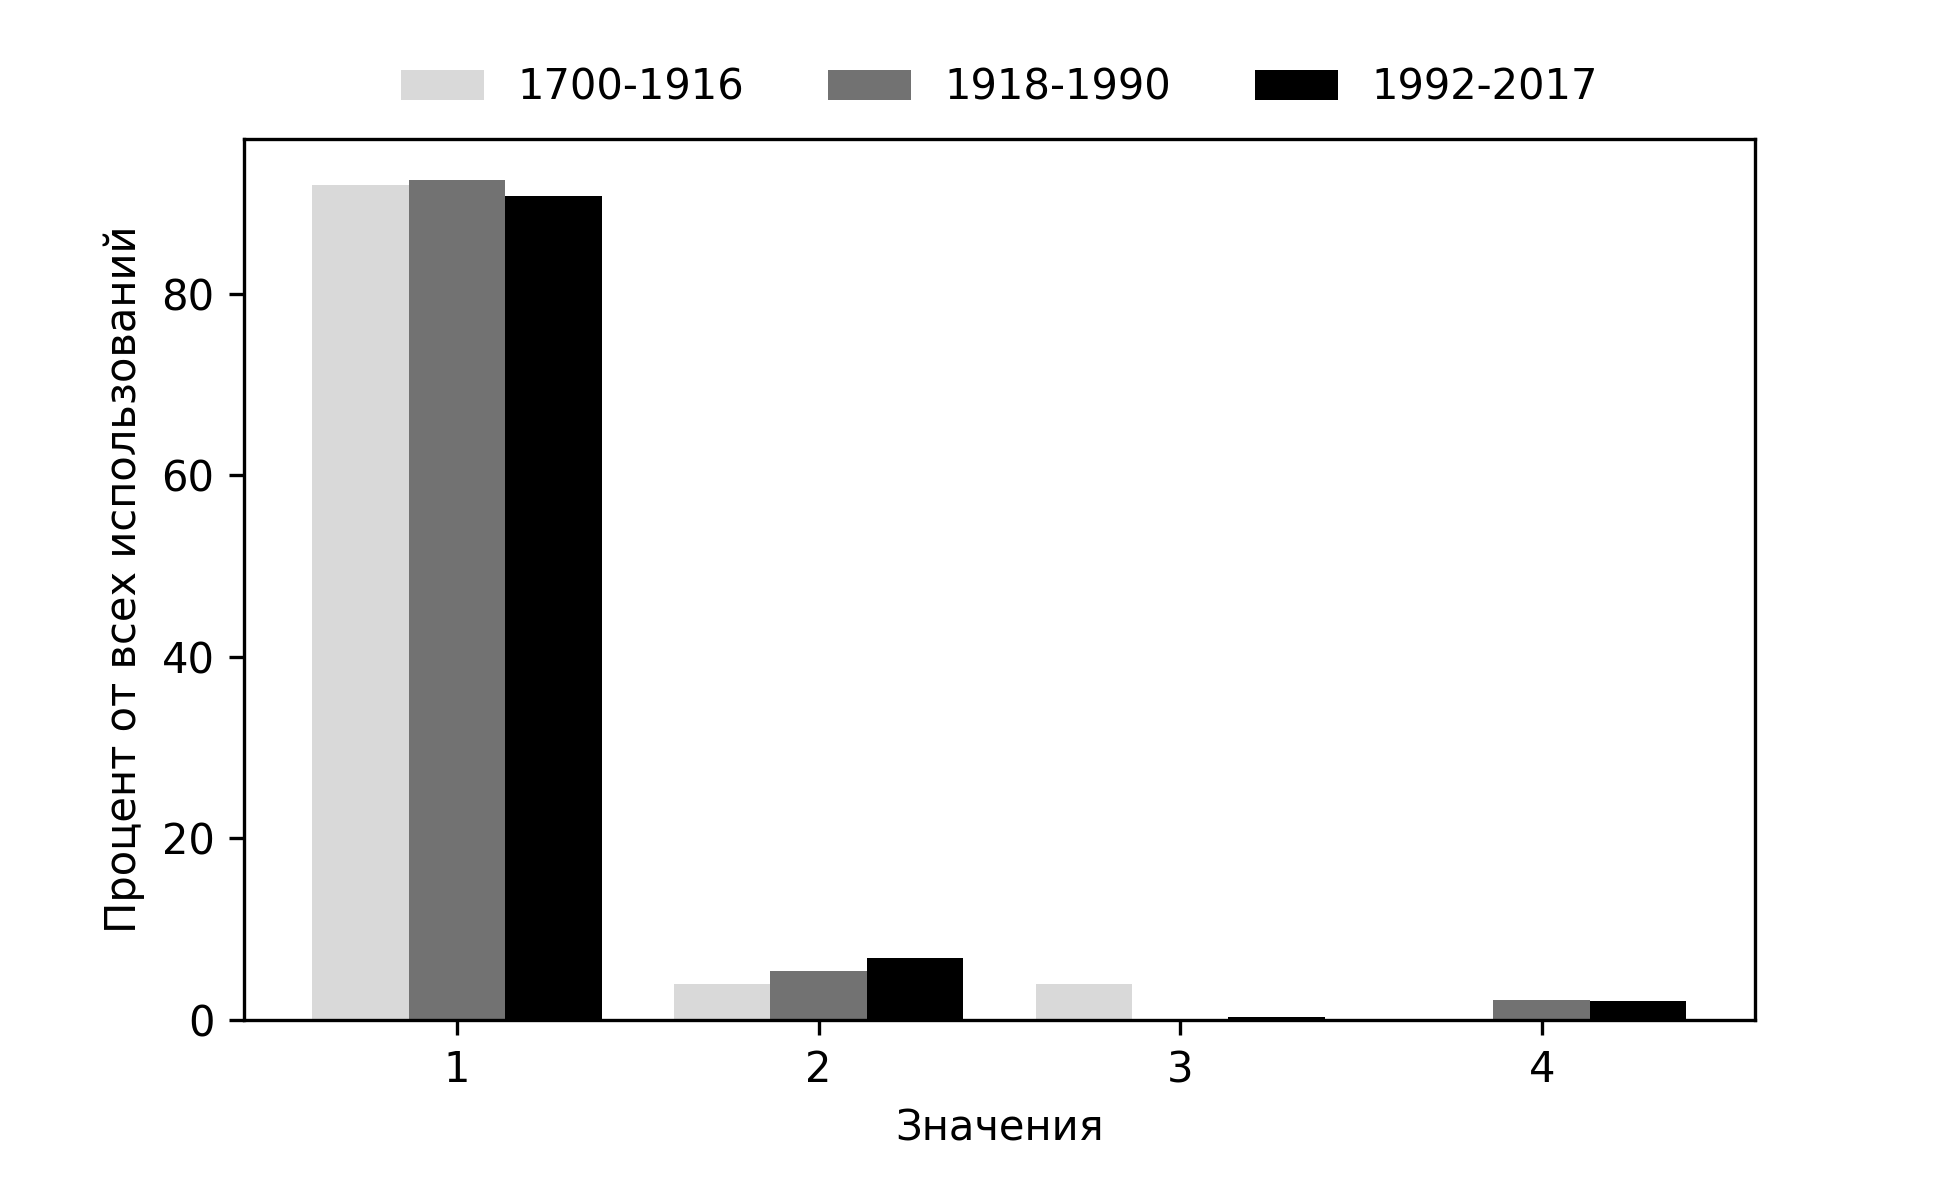
\includegraphics[width=0.8\textwidth]{img/visualizations/znatnyj_minimal}
	\caption{Изменение значений слова \textit{знатный}}
	\label{fig:Знатный}
\end{figure}

Значения для визуализации слова \textit{знатный} (Параметры: eps=0.2, min\_samples=10).

\begin{enumerate}
    \item Принадлежащий к знати, имеющий высокое общественное положение.
    \item Очень хороший, превосходный.
    \item Значительный по значению, важный, значительный.
    \item Знающий свое дело, искусный, опытный.
\end{enumerate}

\subsection*{Анализ значений слова \textit{знатный}}

Первое и второе определения корректно сформулированы.
Третье и четвертое определения соответствуют обобщенным значениям.
Пятое определение не соответствует обобщенным значениям.

\begin{itemize}
    \item ’Принадлежащий к знати, имеющий высокое общественное положение.’ имеет общий смысловой элемент с
’Принадлежащий к знати, к аристократии, к верхушке привилегированного класса.’,
а именно семы \textit{’принадлежность к знати’}, \textit{’высокое общественное положение’}.

    \item ’Очень хороший, превосходный.’ полностью соответствует ’Отличный, высокий по качеству.’,
так как включает те же семы \textit{’отличный’}, \textit{’высокий по качеству’}, \textit{vпревосходный’}.

    \item ’Значительный по значению, важный, значительный.’ соответствует
’Существенный, серьезный (усилитель).’, так как включает те же семы \textit{’важность’}, \textit{’серьезность’}.

    \item ’Знающий свое дело, искусный, опытный.’ частично соответствует
’Известный, знаменитый, прославленный своей деятельностью.’,
так как включает семы \textit{’искусный’}, \textit{’опытный’}, которые подразумевают известность и признание в своей деятельности.
\end{itemize}

Обобщённые значения, не найденные в визуализации:
\begin{itemize}
    \item ’Знаемый, известный, видимый’ также отсутствует в визуализации.
Это значение могло быть не выделено из-за недостаточной частотности.
\end{itemize}

Таким образом, для лексемы \textit{знатный} представлено 3 корректных определения.
Среди ошибок присутствуют:
\begin{itemize}
    \item Близкие: 1
\end{itemize}

Перейдем к частотности значений.

Информация из «Двух веков в двадцати значениях» представлена на графиках~\ref{fig:TwoCentruriesZnatniy1} и~\ref{fig:TwoCentruriesZnatniy2}
В книге можно выделить три основных момента.
Во-первых, наличие до конца XVIII века значения ’Знаемый, известный, видимый’,
однако оно не было выделено алгоритмом.
Во-вторых, преимущественное использование значения
’Принадлежащий к знати, имеющий высокое общественное положение.’ на протяжении
всего исследуемого времени.
Такой же результат наблюдается и в визуализации, с 90\% использования на протяжении трех эпох.
В-третьих, появление в советский период значения, связанного с трудом,
что так же отражается на построенном графике.

\noindent % Prevents indentation for this line to align the images at the left margin
\begin{figure}[H]
    \centering % Centers the images
    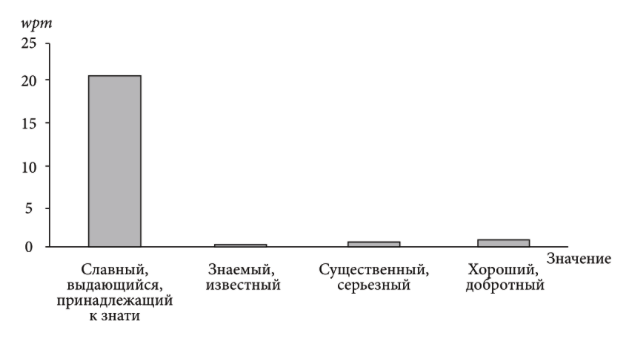
\includegraphics[width=0.8\textwidth]{img/book/znatnij/1891-1920}
    \caption{График для слова \textit{Знатный} для 1891-1920 согласно~\cite{TwoCenturies}}
    \label{fig:TwoCentruriesZnatniy1}
\end{figure}

%\begin{figure}[H]
%    \centering % Centers the images
%    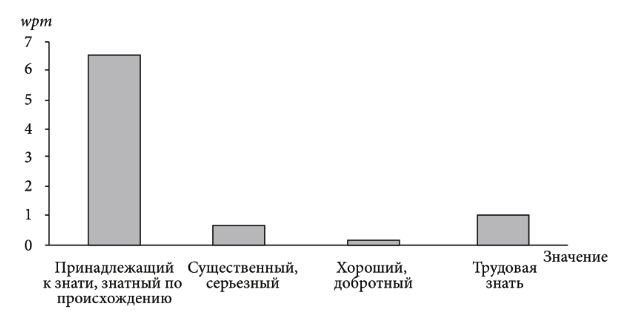
\includegraphics[width=0.8\textwidth]{img/book/znatnij/1921-1950}
%    \caption{Second Image Caption}
%\end{figure}

\begin{figure}[H]
    \centering % Centers the images
    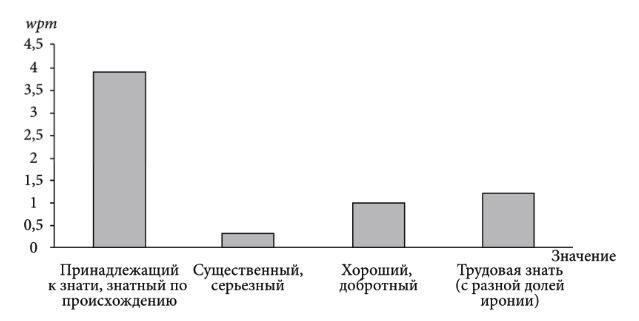
\includegraphics[width=0.8\textwidth]{img/book/znatnij/1990-2010}
    \caption{График для слова \textit{Знатный} для 1990-2010 согласно~\cite{TwoCenturies}}
    \label{fig:TwoCentruriesZnatniy2}
\end{figure}

Таким образом, алгоритм в целом отражает значения, в которых использовалось
слово \textit{знатный}, согласуясь с данными из толкового словаря и историческим исследованием.
Алгоритм выделяет как основное значение, связанное с высоким положением, так и большинство
менее частых.

\section*{Кануть}

В результате анализа семем лексемы \textit{кануть} в толковых словарях были выделены четыре группы значений,
которые можно условно сформулировать следующим образом:

\begin{enumerate}
    \item Упасть каплей; капнуть. \textit{Канула слеза.}
    (\textit{«Упасть каплей; капнуть.»} в БТС,
    \textit{«Капнуть, упасть каплей (устар.).»} в ТСО,
    \textit{«Капнуть.»} в «Двух веках в двадцати словах»)

    \item Погрузиться, утонуть. \textit{Канул на дно реки.}
    (\textit{«Упав куда-л., во что-л., погрузиться.»} в БТС,
    \textit{«Утонуть, упасть на дно.»} в «Двух веках в двадцати словах»)

    \item Бесследно исчезнуть, пропасть. \textit{Куда же он канул?}
    (\textit{«Пропасть, исчезнуть, скрыться.»} в БТС,
    \textit{«Бесследно пропасть, исчезнуть.»} в ТСО,
    \textit{«Пройти, минуть, исчезнуть.»} в «Двух веках в двадцати словах»)

    \item Исчезнуть из виду. \textit{А потом канет дорога в сосняк.}
    (\textit{«Исчезнуть из виду.»} в «Двух веках в двадцати словах»)
\end{enumerate}

%Выражения (фразеологизмы):
%\begin{itemize}
%    \item Кануть в Лету. Быть забытым, бесследно исчезнуть.
%    (\textit{«Кануть в Лету (быть забытым, бесследно исчезнуть).»} в БТС,
%    \textit{«Кануть в Лету (бесследно исчезнуть из памяти людей; высок.; в греческой мифологии Лета — река забвения).»} в ТСО)
%
%    \item Как (будто, словно) в воду канул. Исчезнуть, пропасть бесследно.
%    (\textit{«Как (будто, словно) в воду канул. Исчез, пропал бесследно.»} в БТС,
%    \textit{«Как в воду канул кто бесследно исчез.»} в ТСО)
%\end{itemize}

\begin{figure}[H]
	\centering
	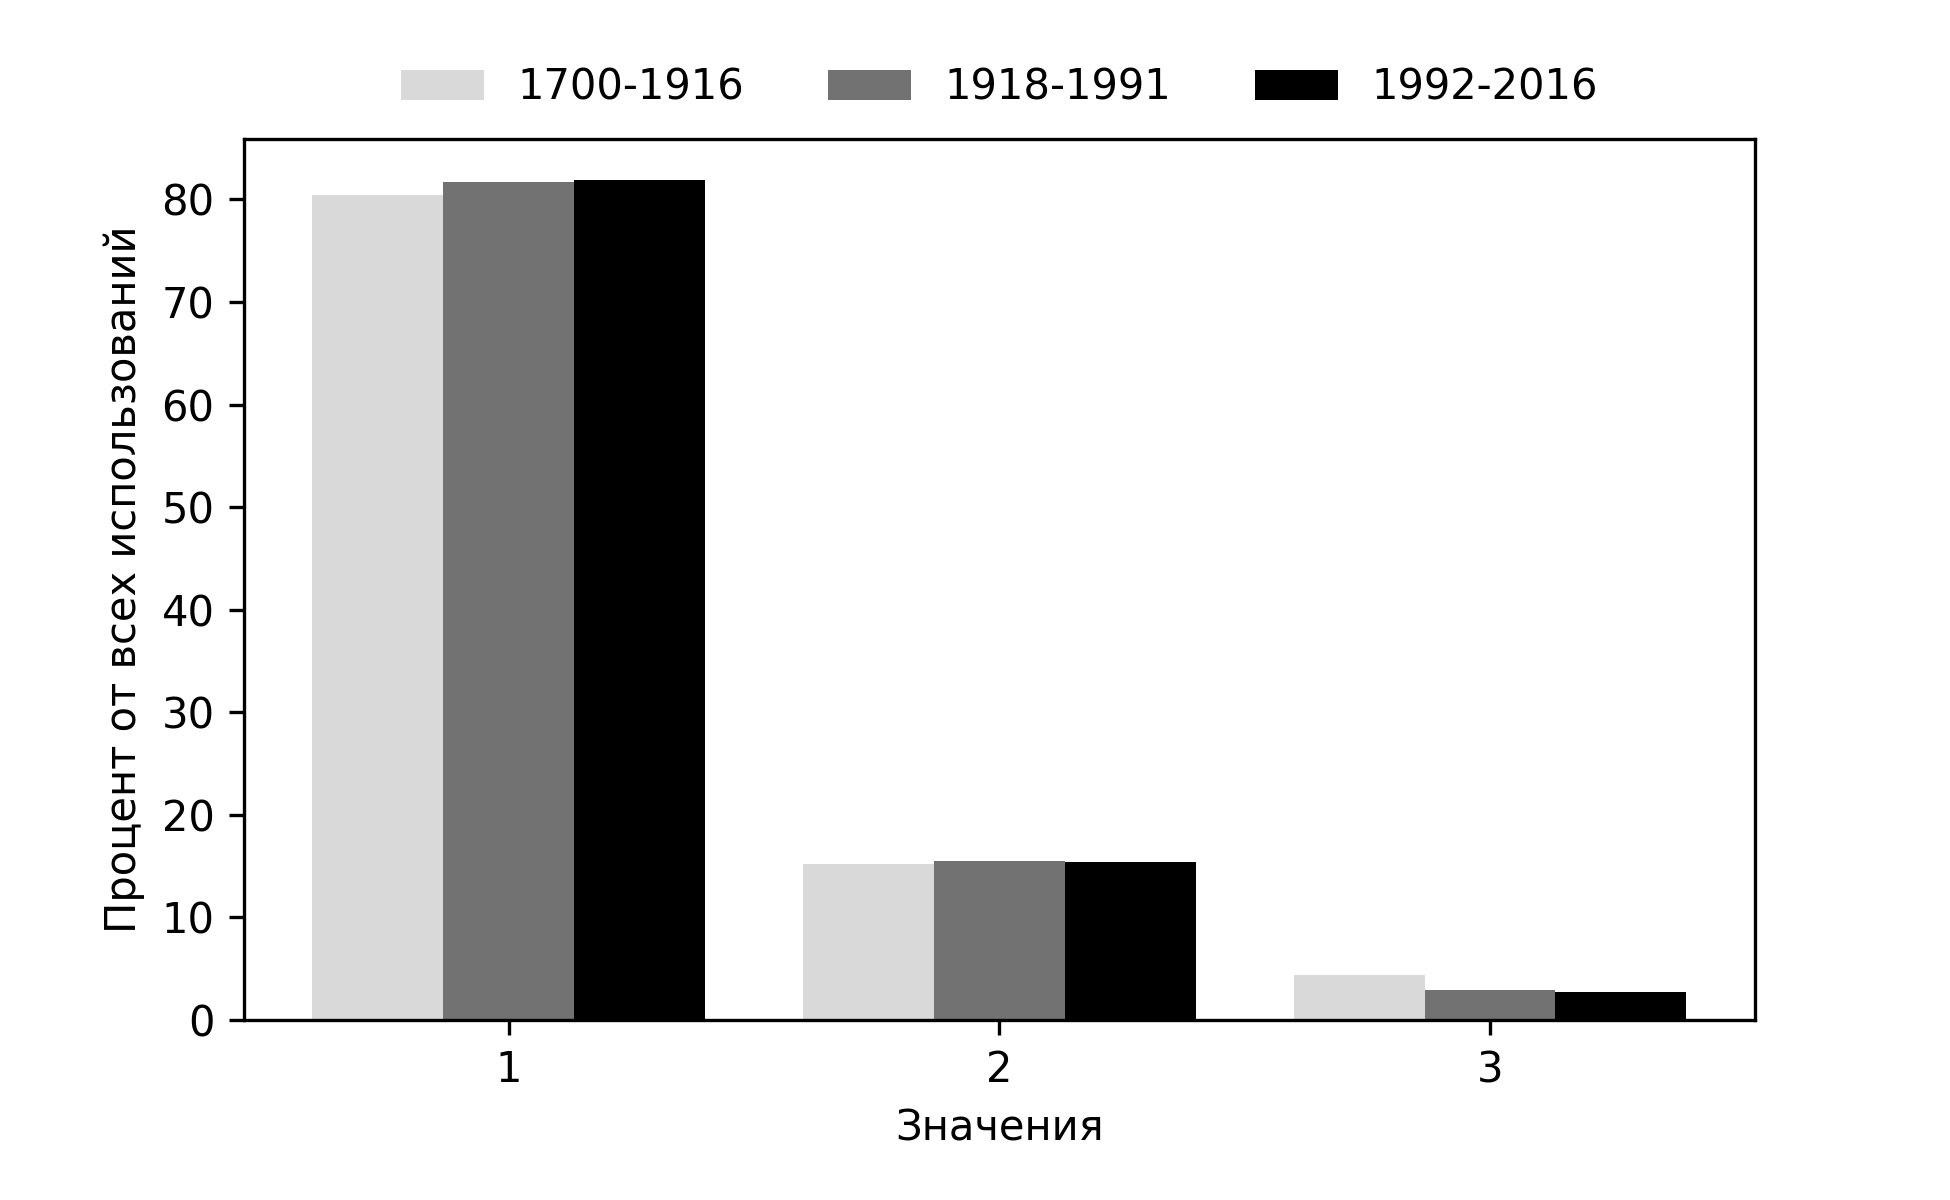
\includegraphics[width=0.8\textwidth]{img/visualizations/kanut'_minimal}
	\caption{Изменение значений слова \textit{кануть}}
	\label{fig:Кануть}
\end{figure}

Значения для визуализации слова \textit{кануть} (Параметры: eps=0.18, min\_samples=10).

\begin{enumerate}
    \item Исчезнуть, пропасть.
    \item Пройти, миновать, исчезнуть.
    \item Упасть, погрузиться.
\end{enumerate}

\subsection*{Анализ значений слова \textit{кануть}}

Первые три определения корректно сформулированы.

\begin{itemize}
    \item ’Исчезнуть, пропасть.’ корректное определение, так как имеет общий смысловой элемент с
’Бесследно исчезнуть, пропасть.’, а именно семы \textit{’исчезнуть’} и \textit{’пропасть’}.

    \item ’Пройти, миновать, исчезнуть.’ частично соответствует
’Бесследно исчезнуть, пропасть.’ и ’Исчезнуть из виду.’, так как включает те же семы \textit{пройти’}, \textit{исчезнуть’}.
Визуализация добавляет семы \textit{’миновать’}, что расширяет значение, делая его более широким.

    \item ’Упасть, погрузиться.’ частично соответствует ’Погрузиться, утонуть.’,
так как включает семы \textit{’упасть’} и \textit{’погрузиться’}.
\end{itemize}

\begin{itemize}
    \item ’Упасть каплей; капнуть.’ не выделяется алгоритмом.
Можно предположить, что это значение недостаточно часто встречается.
В «Двух веках в двадцати словах» указано, что на протяжении XIX века оно заменяется
другими значениями.
\end{itemize}

Таким образом, для лексемы \textit{кануть} представлено 1 корректное определение.
Среди ошибок присутствуют:
\begin{itemize}
    \item Близкие значения: 2
\end{itemize}

Перейдем к частотности значений.

Затруднительно провести анализ рассматриваемого слова,
так как, судя по «Двум векам в двадцати словах» выделенные алгоритмом значения появляются
в досоветский период и продолжают использоваться дальше.
Подтверждается информация о том, что с 1900 года ’исчезнуть, сгинуть, пропасть’ является
основным значением слова, однако книга не предоставляет визуализаций частоты
использования значений слова по периодам.

\section*{Классный}

В результате анализа семем лексемы \textit{классный} в толковых словарях были выделены пять групп значений,
которые можно условно сформулировать следующим образом:

\begin{enumerate}
    \item Имеющий отношение к школьному обучению. \textit{Классная доска.}
(\textit{«к Класс (3 зн.)»} в БТС,
\textit{«Классным называют то, что имеет отношению к классу.»} в ТСД,
\textit{«Имеющий отношение к школьному обучению.»} в «Двух веках в двадцати словах»)

    \item Имеющий определённый класс, разряд, соответствующий требованиям такого класса, разряда. \textit{Классы морских судов.}
(\textit{«Имеющий определённый класс, разряд, соответствующий требованиям такого класса, разряда.»} в БТС,
\textit{«Имеющий класс (разряд).»} в «Двух веках в двадцати словах»)

    \item Имеющий определённый ранг, чин. \textit{Небольшой классный чиновник.}
(\textit{«Имеющий определённый ранг, чин.»} в БТС,
\textit{«Классный чиновник.»} в «Двух веках в двадцати словах»)

    \item Специалист, обладающий высоким мастерством в своей области. \textit{Классный водитель.}
(\textit{«Принадлежащий к высшему классу, разряду по квалификации, по мастерству в чём-л.»} в БТС,
\textit{«Классным называют специалиста, который обладает высоким мастерством в своей области.»} в ТСД)

    \item Отличный, высокого качества. \textit{Обед был классный!}
(\textit{«Отличный.»} в БТС,
\textit{«Принадлежащий к высшему классу (в 4 знач.), высокого качества (разг.).»} в ТСО,
\textit{«Классным называют человека, предмет, событие и т. п., которые имеют замечательные свойства,
обладают высоким качеством; разговорный стиль.»} в ТСД,
\textit{«Хороший, отличный.»} в «Двух веках в двадцати словах»)
\end{enumerate}

\begin{figure}[H]
	\centering
	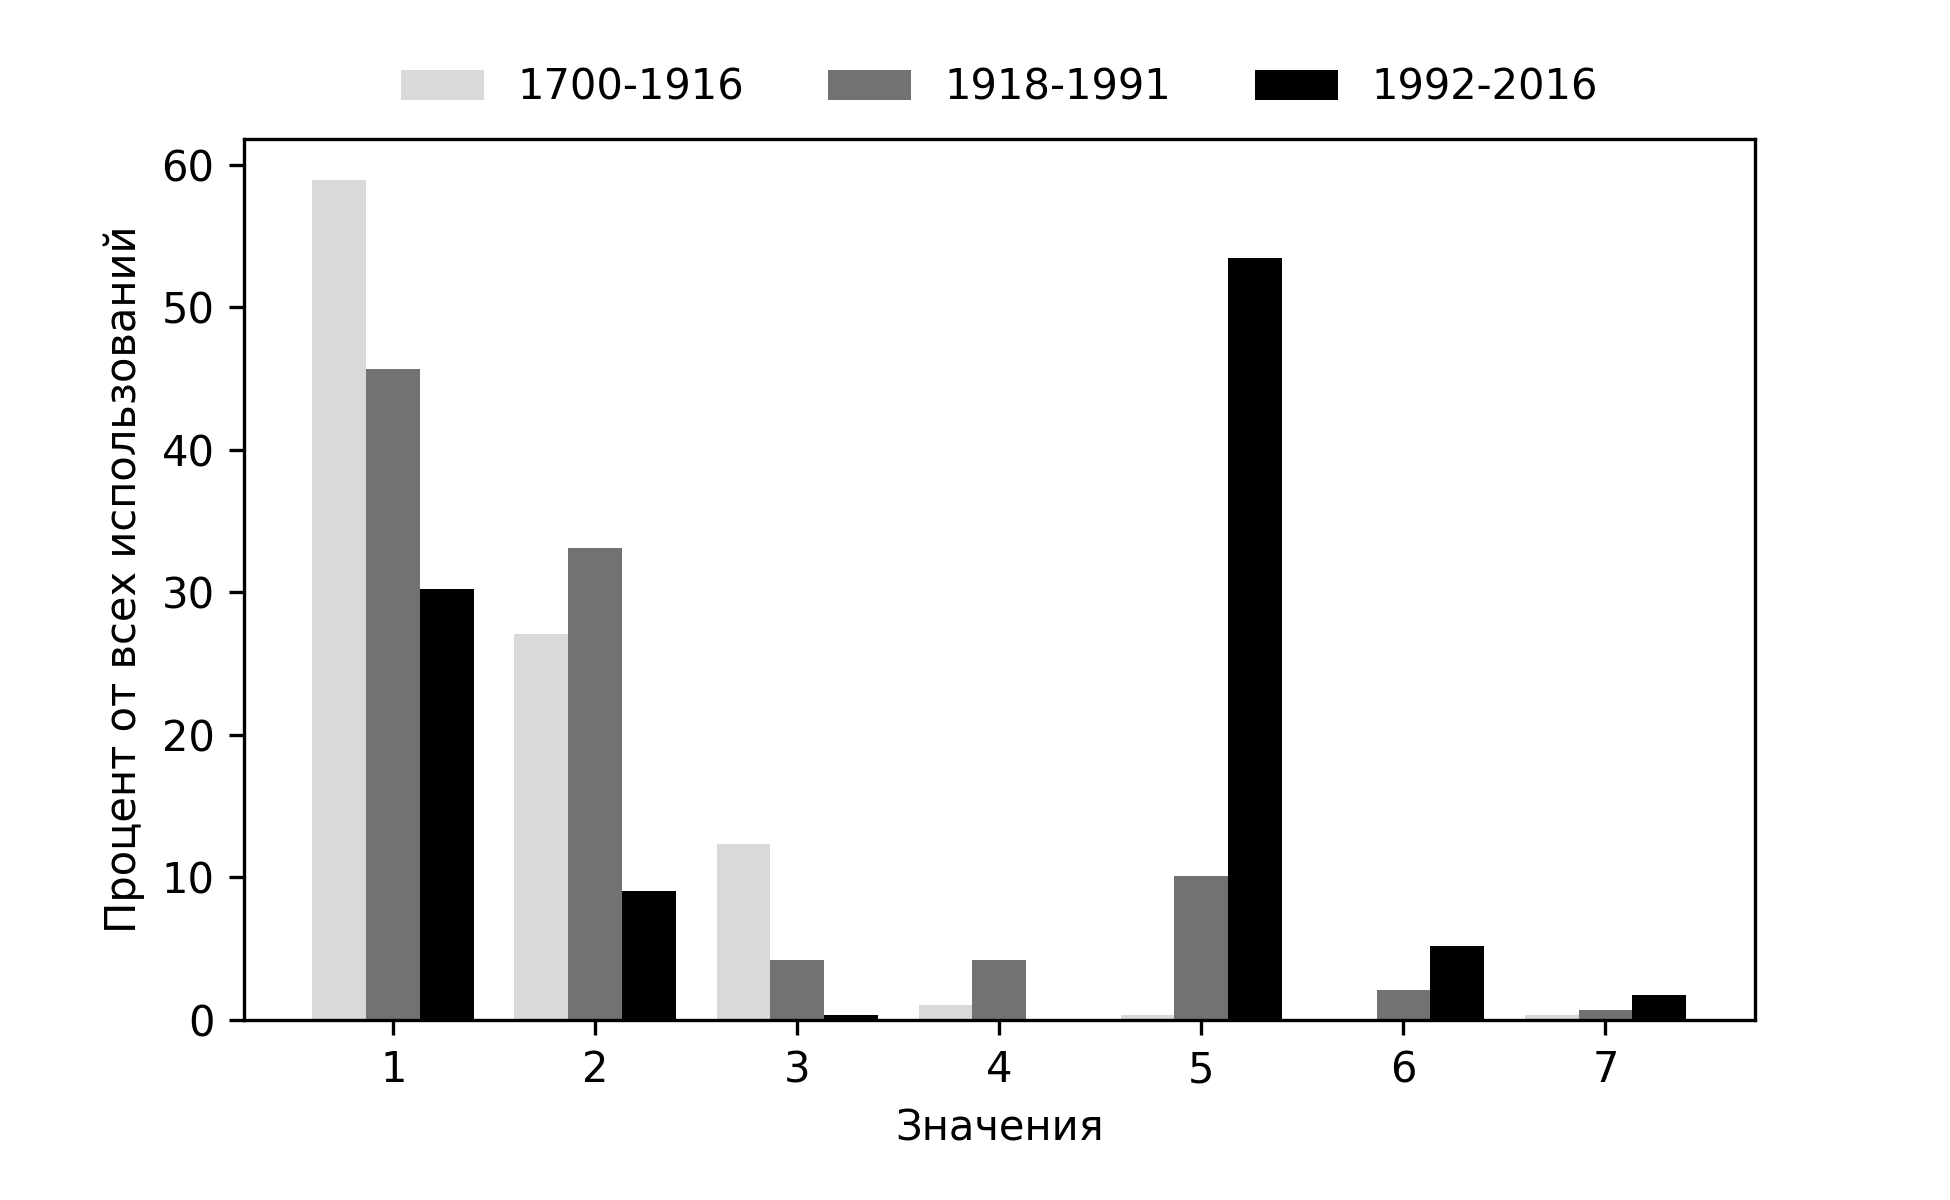
\includegraphics[width=0.8\textwidth]{img/visualizations/klassnyj_minimal}
	\caption{Изменение значений слова \textit{классный}}
	\label{fig:Классный}
\end{figure}

Значения для визуализации слова \textit{классный} (Параметры: eps=0.22, min\_samples=5).

\begin{enumerate}
    \item Служащий в классе, занимающийся в классе.
    \item Предназначенный для класса.
    \item Помещение для занятий в школе.
    \item Предназначенный для пассажиров первого класса.
    \item Очень хороший, замечательный.
    \item Отличающийся высоким мастерством в каком-л. деле.
    \item Связанный с присвоением какого-либо звания, чина.
\end{enumerate}

\subsection*{Анализ значений слова \textit{классный}}

Третье и четвертое определения не соответствуют обобщенным значениям.
Остальные определения являются корректными.

\begin{itemize}
    \item ’Служащий в классе, занимающийся в классе.’ соответствует определению
’Имеющий отношение к школьному обучению.’, объединяя семы \textit{’служащий’}, \textit{’занимающийся’}, \textit{’класс’}.

    \item ’Предназначенный для класса.’ также относится к определению
’Имеющий отношение к школьному обучению.’ с теми же семами.

    \item ’Очень хороший, замечательный.’ соответствует значению ’Отличный, высокого качества.’,
объединяя семы \textit{’хороший’}, \textit{’отличный’}, \textit{’высокого качества’}.

    \item ’Отличающийся высоким мастерством в каком-л. деле.’ соответствует значению
’Специалист, обладающий высоким мастерством в своей области.’,
объединяя семы \textit{’высокий мастерство’}, \textit{’специалист’}, \textit{’область’}.

    \item ’Связанный с присвоением какого-либо звания, чина.’ аналогично определению
’Имеющий определённый ранг, чин.’, объединяя семы \textit{’звание’}, \textit{’чин’}, \textit{’ранг’}.
\end{itemize}

Слишком специфичные значения:
\begin{itemize}
    \item ’Помещение для занятий в школе.’ является слишком специфичным
и может быть включено в ’Имеющий отношение к школьному обучению.’

    \item ’Предназначенный для пассажиров первого класса.’ также является слишком специфичным,
может быть включено в ’Имеющий определённый класс, разряд, соответствующий требованиям такого класса, разряда.’.
\end{itemize}

Таким образом, для лексемы \textit{классный} представлено 5 корректных определений.
Среди ошибок присутствуют:
\begin{itemize}
    \item Избыточное конкретизирование: 2
\end{itemize}

Перейдем к частотности значений.

Основными моментами из книги «Два века в двадцати словах» является появление
в советское время значения ’Очень хороший, замечательный.’,
становление его основным в постсоветский период и
преобладание значений, связанных со школой, до этого.
Всё вышеперечисленное выводится из нашей визуализации,
где значение ’Очень хороший, замечательный.’ набирает около 10\% от всех
использований в советский период и около 55\% в постсоветский.
Значения, связанные со школьным обучением (1, 2, 3) вместе набирают
более 90\% от всех использований в досоветский период.
Информация из книги «Два века в двадцати словах» приведена в графике~\ref{fig:TwoCenturiesKlassnij}.

\begin{figure}[H]
    \centering % Centers the images
    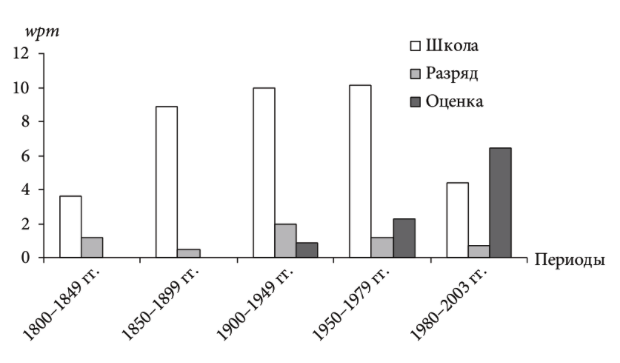
\includegraphics[width=0.8\textwidth]{img/book/klassnij/all}
    \caption{График для слова \textit{Классный} согласно~\cite{TwoCenturies}}
    \label{fig:TwoCenturiesKlassnij}
\end{figure}

Таким образом, алгоритм отражает значения, в которых использовалось
слово \textit{классный}, согласуясь с данными из толкового словаря и историческим исследованием,
однако некоторые определения являются слишком специфичными.

\section*{Мама}

В результате анализа семем лексемы \textit{мама} в толковых словарях были выделены
пять групп значений, которые можно условно сформулировать следующим образом:

\begin{enumerate}
    \item Женщина, являющаяся родительницей ребёнка. \textit{Родная мама.}
(\textit{«Женщина по отношению к своим детям»} в ТСО,
\textit{«Женщина по отношению к рождённым ею детям»} в БТС и ТСД,
\textit{«Генетическая мать»} в «Двух веках в двадцати словах»)

    \item Обращение ребёнка к своей матери. \textit{Мам, дай поесть.}
(\textit{«Мамой ребёнок называет свою мать»} в ТСД,
\textit{«Мама — это обращение ребёнка к своей матери»} в ТСД)

    \item Обращение к тёще или свекрови. \textit{Мама приехала в гости.}
(\textit{«Тёща или свекровь (обычно в семейном обращении)»} в БТС,
\textit{«Мамой в разговорной речи иногда называют тёщу или свекровь»} в ТСД)

    \item Обращение к опекуну или кормильцу без родственных связей. \textit{Мамы не прикармливали пряниками тихонько, а дядьки не дирали за уши за все про все.}
(\textit{«Комилица, няня»} в «Двух веках в двадцати словах»)

    \item Наименование компонента компьютера – материнской платы. \textit{Покупка же новой «мамы» вместе с процессором тянет на 200 долларов.}
(\textit{«Материнская плата»} в «Двух веках в двадцати словах»)
\end{enumerate}

\begin{figure}[H]
	\centering
	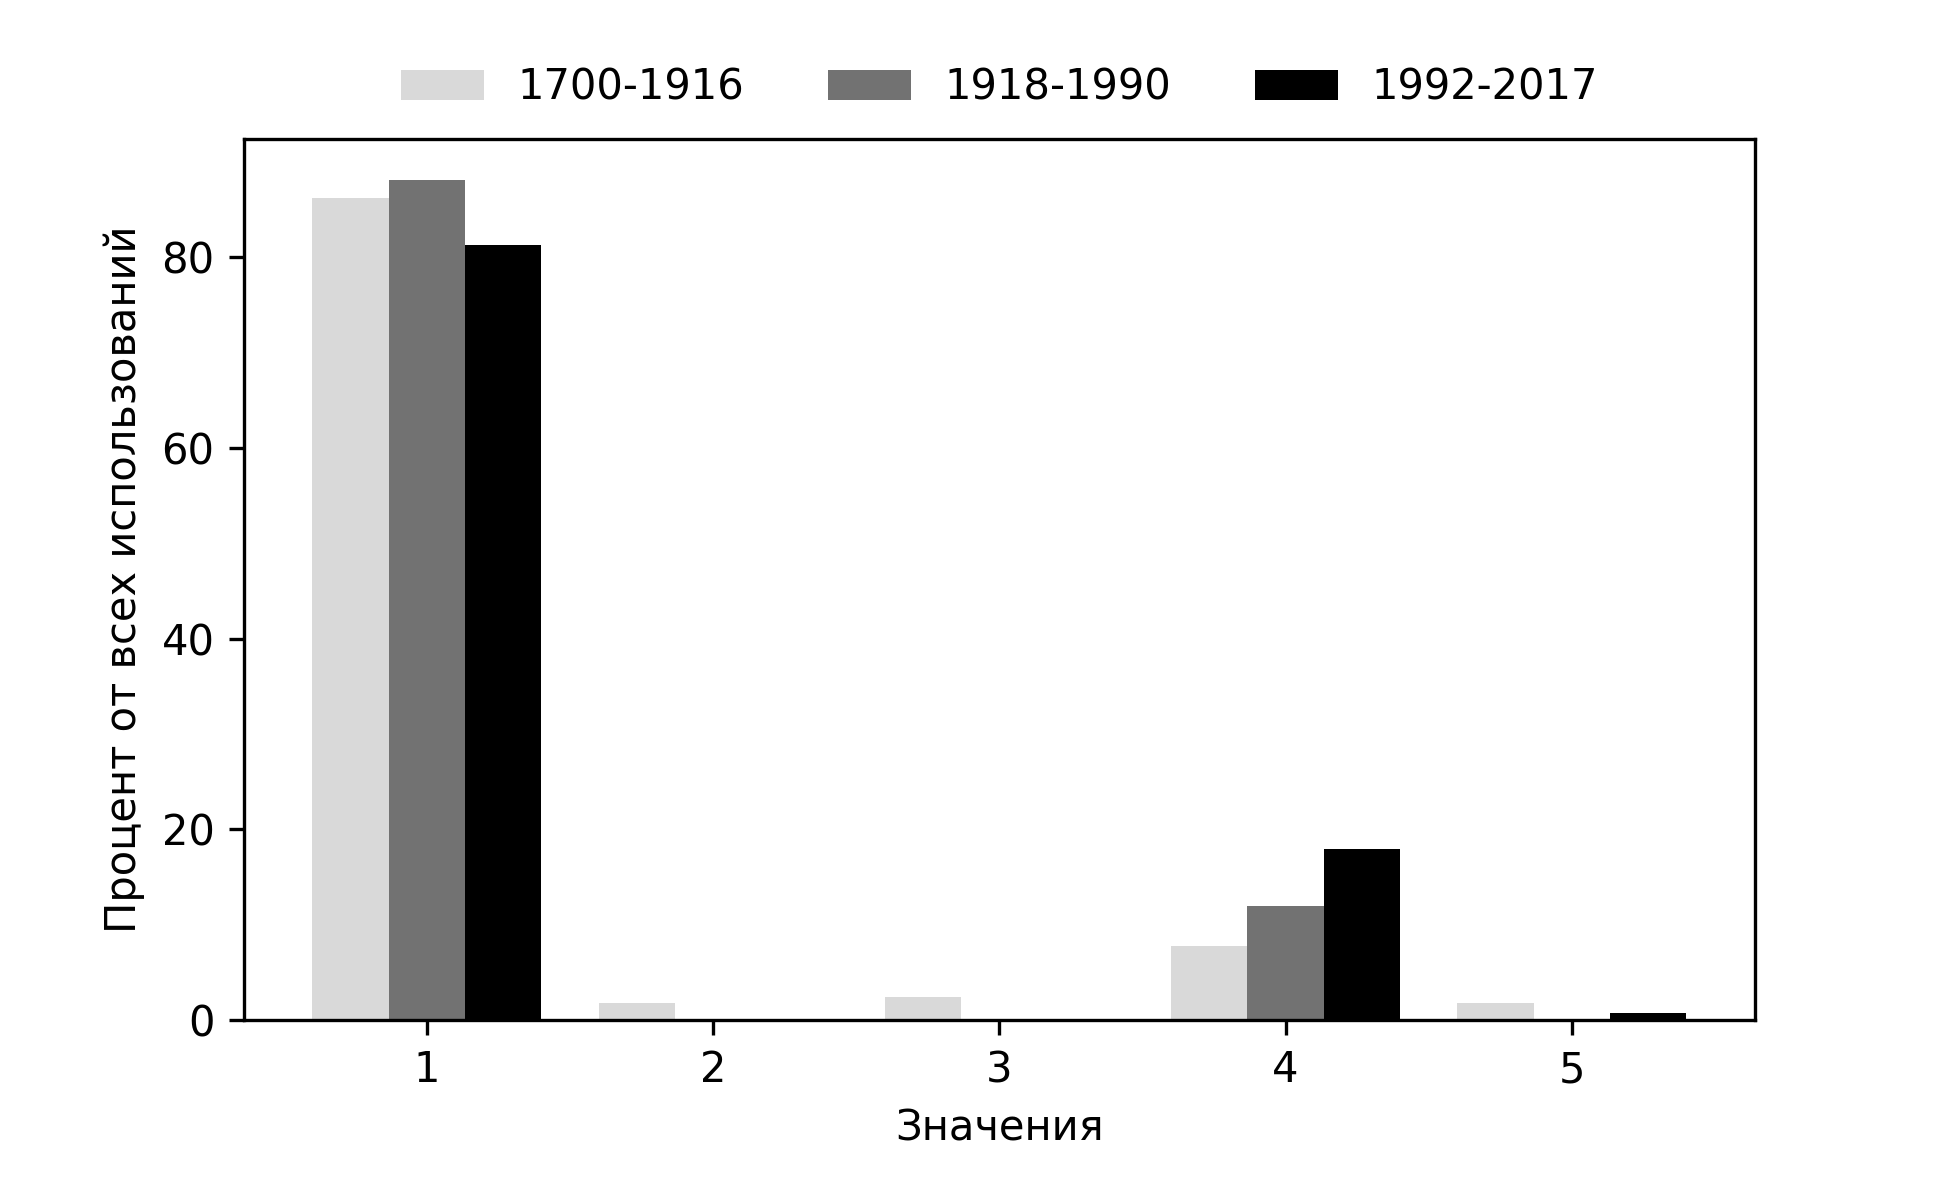
\includegraphics[width=0.8\textwidth]{img/visualizations/mama_minimal}
	\caption{Изменение значений слова \textit{мама}}
	\label{fig:Мама}
\end{figure}

Значения для визуализации слова \textit{мама} (Параметры: eps=0.08, min\_samples=5).

\begin{enumerate}
    \item Женщина, мать.
    \item Фамильярное обращение к пожилому мужчине.
    \item В дореволюционной России: женщина, занимавшаяся воспитанием детей.
    \item Женщина по отношению к своим детям.
    \item Ласковое обращение к женщине.
\end{enumerate}

\subsection*{Анализ значений слова \textit{мама}}

Первое, третье и четвертое определения корректно сформулированы.
Второе и пятое определения не соответствуют обобщенным значениям.

\begin{itemize}
    \item ’Женщина, мать.’ имеет общий смысловой элемент с
’Женщина, являющаяся родительницей ребёнка.’, а именно семы \textit{’женщина’} и \textit{’родитель’}.

    \item ’Женщина по отношению к своим детям.’ полностью соответствует
’Женщина, являющаяся родительницей ребёнка.’, так как включает те же семы \textit{’женщина’}, \textit{’родитель’}.

    \item ’В дореволюционной России: женщина, занимавшаяся воспитанием детей.’ имеет соответствие с
’Обращение к опекуну или кормильцу без родственных связей.’,
так как семы \textit{’женщина’}, \textit{’занимающаяся воспитанием детей’} отражают смысл ’няня’.
\end{itemize}

\begin{itemize}
    \item ’Фамильярное обращение к пожилому мужчине.’ является некорректным значением,
в обобщенных значениях нет упоминаний о мужчине.

    \item ’Ласковое обращение к женщине.’ близко к
’Обращение ребёнка к своей матери.’, но имеет более широкий смысл, включающий всех женщин,
а не только матерей или нянь, что делает его недостаточно специфичным.
\end{itemize}

Обобщённые значения, не найденные в визуализации:
\begin{itemize}
    \item ’Обращение к тёще или свекрови’ отсутствует среди предложенных моделью значений.
Можно предположить, что информации из контекста использований недостаточно для отделения
этого значения от ’женщина, мать.’.

    \item ’Наименование компонента компьютера – материнской платы’ также отсутствует в визуализации.
Однако, модель способна на выделение данного значения.  % TODO: прогнать на примере модель
\end{itemize}

Таким образом, для лексемы \textit{мама} представлено 3 корректных определения:
Среди ошибок присутствуют:
\begin{itemize}
    \item Некорректность определения: 1
    \item Недостаточное конкретизирование: 1
\end{itemize}

Перейдем к частотности значений.

Основным моментом в Двух веках в двадцати словах для слова \textit{мама}
является появление значения ’Женщина, являющаяся родительницей ребёнка.’, сменивашего
’Обращение к опекуну или кормильцу без родственных связей.’ в середине XIX века.
Это отражено в визуализации алгоритма, где ’В дореволюционной России: женщина, занимавшаяся воспитанием детей.’
присутствует только для досоветского периода.
Основным значением для остальных периодов является ’Женщина, являющаяся родительницей ребёнка.’,
что также отражено в визуализации алгоритма.
Информация из книги приведена в графике~\ref{fig:TwoCenturiesMom}.
Также в книге упоминается появление значения ’Наименование компонента компьютера – материнской платы’
в конце XX века, однако он не был выделен алгоритмом.

\begin{figure}[H]
    \centering % Centers the images
    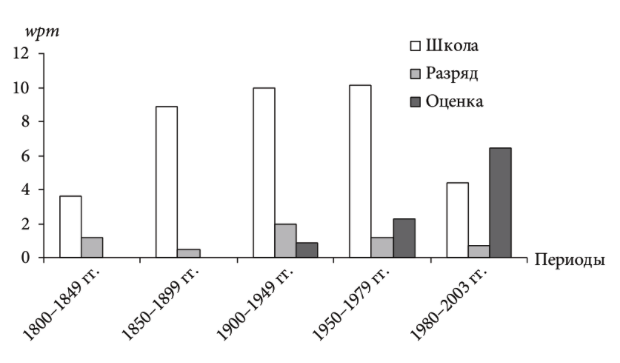
\includegraphics[width=0.8\textwidth]{img/book/klassnij/all}
    \caption{График для слова \textit{Мама} для 1760-1889 согласно~\cite{TwoCenturies}}
    \label{fig:TwoCenturiesMom}
\end{figure}

Таким образом, алгоритм отражает часть значений, в которых использовалось
слово \textit{мама}, согласуясь с данными из толкового словаря и историческим исследованием.
Часть значений предложена некорректно, так как в них упоминается употребление слова по отношению
к мужчинам, а также по отношению к абсолютно всем женщинам.

\section*{Анализ слова \textit{машина}}

В результате анализа семем лексемы \textit{машина} в толковых словарях были выделены девять групп значений,
которые можно условно сформулировать следующим образом:

\begin{enumerate}
    \item Механическое устройство, совершающее полезную работу с преобразованием энергии, материалов или информации. \textit{Вязальная машина.}
(\textit{«Механизм или совокупность механизмов, совершающие какую-л. полезную работу путём преобразования одного вида энергии в другой.»} в БТС,
\textit{«Механическое устройство, совершающее полезную работу с преобразованием энергии, материалов или информации.»} в ТСО,
\textit{«Машина — это механизм, который совершает какую-либо полезную работу.»} в ТСД,
\textit{«Бытовой прибор»} в «Двух веках в двадцати словах»)

    \item Автомобиль, средство передвижения. \textit{Спортивная гоночная машина.}
(\textit{«Автомобиль, автомашина.»} в БТС,
\textit{«То же, что автомобиль.»} в ТСО,
\textit{«Машина — это средство передвижения, автомобиль.»} в ТСД,
\textit{«Автомобиль»} в «Двух веках в двадцати словах»)

    \item Организация, действующая подобно механизму, налаженно, чётко, бесперебойно. \textit{Военная машина.}
(\textit{«О какой-л. организации, ведомстве и т.п., действующих, подобно механизму, бесперебойно, точно, ритмично.»} в БТС,
\textit{«Об организации, действующей подобно механизму, налаженно и чётко.»} в ТСО,
\textit{«Машиной называют политическую, военную и т. п. организации, которые действуют точно и бесперебойно, как механизм.»} в ТСД)

    \item Человек, лишённый каких-либо эмоций, действующий машинально, автоматически. \textit{Не человек, а машина.}
(\textit{«О человеке, лишённом каких-л. эмоций, действующем машинально, автоматически.»} в БТС,
\textit{«Машиной в разговорной речи называют человека, который никак не проявляет своих чувств, эмоций и совершает поступки машинально, автоматически.»} в ТСД)

    \item Количество груза, вмещающееся в кузов грузового автомобиля. \textit{Привести машину дров.}
(\textit{«О количестве груза, вмещающегося в кузов грузового автомобиля (обычно от 3 до 5 тонн).»} в БТС,
\textit{«Машиной чего-либо в разговорной речи называют количество груза, которое помещается в одну машину.»} в ТСД)

    \item Движущийся или летающий механизм. \textit{Машины с дистанционным управлением.}
(\textit{«О самодвижущихся механизмах различного значения (комбайне, тракторе, мотоцикле и т.п.).»} в БТС,
\textit{«Машиной называют любой движущийся, летающий механизм.»} в ТСД)

    \item Устройство для работы с информацией, компьютер. \textit{Электронно-вычислительная машина.}
(\textit{«Комплекс технических, аппаратных и программных средств, предназначенных для автоматического сбора, хранения, обработки, передачи информации и её использования.»} в БТС,
\textit{«Компьютер.»} в «Двух веках в двадцати словах»)

    \item Мотоцикл, велосипед. \textit{Выбрать машину, которая лучше всего подходит для трассы.}
(\textit{«У спортсменов: мотоцикл, велосипед.»} в ТСО)

    \item Поезд, паровоз. \textit{Стоявшие по сторонам дороги зрители изумлялись, видя величественное, ровное, легкое, притом скорое движение машины.}
(\textit{«Поезд, паровоз.»} в «Двух веках в двадцати словах»)
\end{enumerate}

\begin{figure}[H]
	\centering
	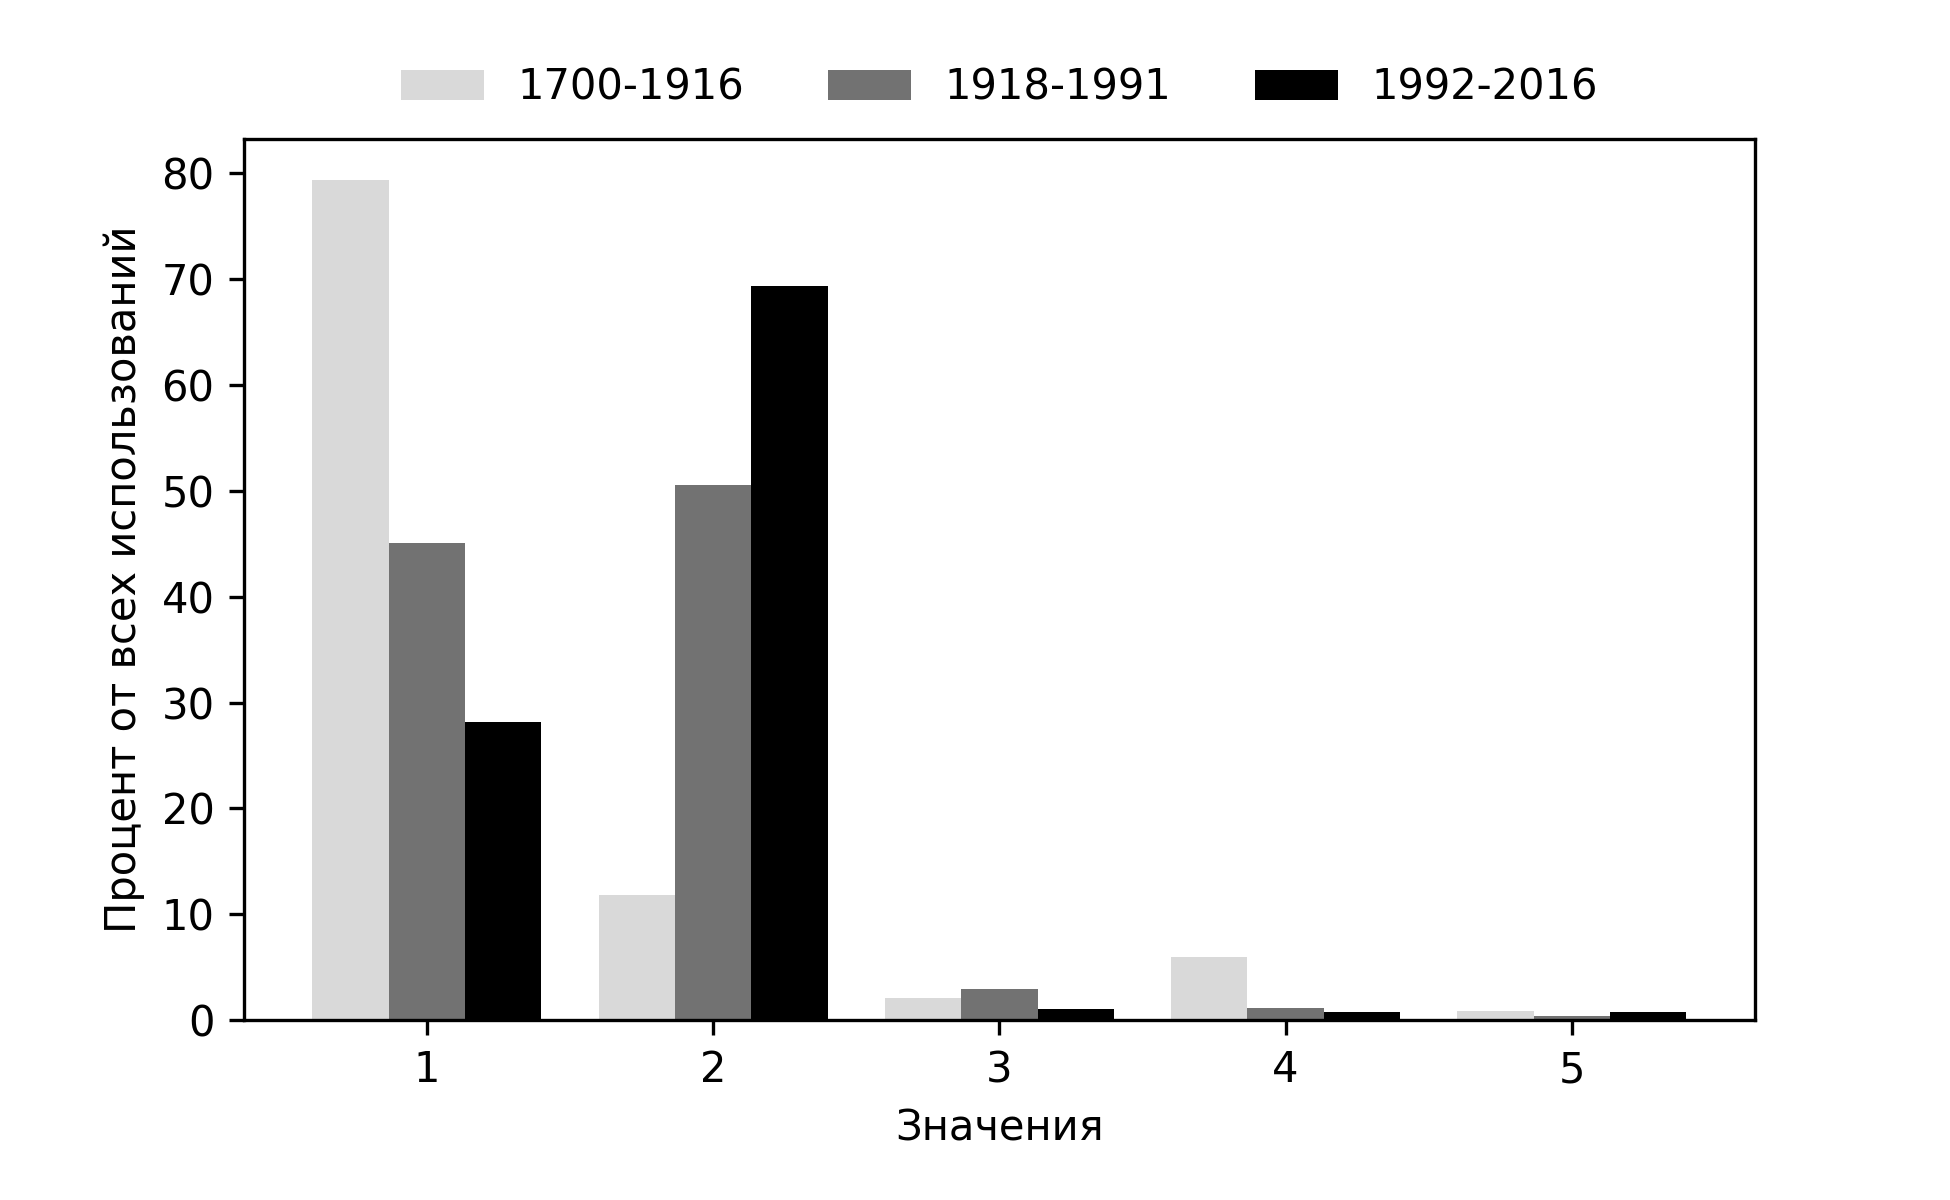
\includegraphics[width=0.8\textwidth]{img/visualizations/mashina_minimal}
	\caption{Изменение значений слова \textit{машина}}
	\label{fig:Машина}
\end{figure}

Значения для визуализации слова \textit{машина} (Параметры: eps=0.15, min\_samples=5).

\begin{enumerate}
    \item Приспособление, устройство, служащее для выполнения какой-л. работы.
    \item Автомобиль, транспортное средство.
    \item Самолет, вертолет и т. п.
    \item О человеке, действующем механически, бездумно.
    \item Система, совокупность каких-либо учреждений, организаций, предприятий и т. п.
\end{enumerate}

\subsection*{Анализ значений слова \textit{машина}}

Первое, второе и четвертое определения корректно сформулированы.
Третье и шестое определения не соответствуют обобщенным значениям.

\begin{itemize}
    \item ’Приспособление, устройство, служащее для выполнения какой-л. работы.’ имеет общий смысловой элемент с
’Механическое устройство, совершающее полезную работу с преобразованием энергии, материалов или информации.’,
а именно семы \textit{’устройство’} и \textit{’выполнение работы’}.
Данное определение корректное.

    \item ’Автомобиль, транспортное средство.’ полностью соответствует
’Автомобиль, средство передвижения.’, так как включает те же семы \textit{’автомобиль’} и \textit{’средство передвижения’}.
Данное определение корректное.

    \item ’О человеке, действующем механически, бездумно.’ имеет общий смысловой элемент с
’Человек, лишённый каких-л. эмоций, действующий машинально, автоматически.’,
а именно семы \textit{’человек’} и \textit{’действующий механически’}.
Данное определение корректное.

    \item ’Система, совокупность каких-либо учреждений, организаций, предприятий и т. п.’ близко к
’Организация, действующая подобно механизму, налаженно, чётко, бесперебойно.’,
так как включает сему \textit{’организация’}, но также включает \textit{’совокупность’},
которой нету у обобщенного определения, но не включает \textit{’слаженность’}, \textit{’чёткость’}, \textit{’бесперебойность’}.% и \textit{’действующая налаженно и чётко’}.
\end{itemize}

\begin{itemize}
    \item Несмотря на то, что как ’Самолет, вертолет и т. п.’ не выделяется среди
обобщённых значений, являясь более узким, чем ’Движущийся или летающий механизм.’,
под обобщённое определение также попадают и другие, как ’Автомобиль, средство передвижения.’
или ’Поезд, паровоз.’, где оба являются типами движущихся механизмов.
В связи с этим на равне с ними представляется разумным признать данное определение как корректное.

%является слишком специфичным значением,
%так как в обобщенных значениях упоминаются самодвижущиеся механизмы различного значения (включая летательные аппараты),
%но не выделяются отдельно.
\end{itemize}

Обобщённые значения, не найденные в визуализации:
\begin{itemize}
    \item ’Количество груза, вмещающееся в кузов грузового автомобиля’ отсутствует среди предложенных моделью значений.
Можно предположить, что информации из контекста использований недостаточно для выделения этого значения.

    \item ’Устройство для работы с информацией, компьютер’ также отсутствует в визуализации.
Однако, модель способна на выделение данного значения.  % TODO: попробововать

    \item Другими отсутствующими значениями являются различные типы транспорта:
’Поезд, паровоз.’ и ’Мотоцикл, велосипед.’.   % TODO: попробововать
\end{itemize}

Таким образом, для лексемы \textit{машина} представлено 4 корректных определений.
Среди ошибок присутствуют:
\begin{itemize}
    \item Близкое значение: 1
\end{itemize}

Перейдем к частотности значений.

’Механическое устройство, совершающее полезную работу с преобразованием энергии,
материалов или информации.’ и схожие с ним значения, судя по «Двум векам в двадцати словах»,
присутствовало в течении всего рассматриваемого периода, что отражается в значении
’Приспособление, устройство, служащее для выполнения какой-л. работы.’, предложенное
нашим алгоритмом.
Однако в течение советского времени ’Автомобиль, средство передвижения.’ становится основным.
Так, на нашей визуализации значение 2 набирает с около 15\% за досоветский период
до около 70\% за постсоветский, данное увеличение произошло в ущерб значению 1 –
’Приспособление, устройство, служащее для выполнения какой-л. работы.’.
Похожая ситуация наблюдается на графиках из книги~\ref{fig:TwoCenturiesMashina1} и~\ref{fig:TwoCenturiesMashina2}.

\noindent % Prevents indentation for this line to align the images at the left margin
\begin{figure}[H]
    \centering % Centers the images
    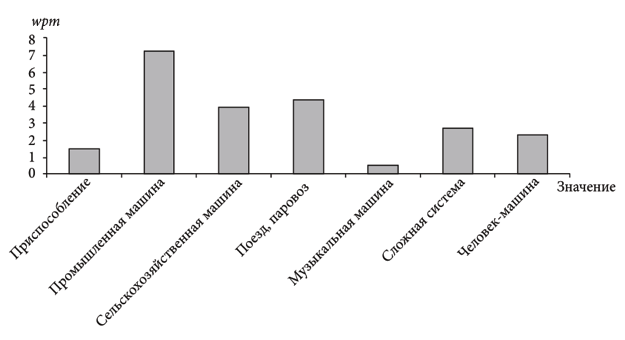
\includegraphics[width=0.8\textwidth]{img/book/mashina/1861-1890}
    \caption{График для слова \textit{машина} для 1861-1890 согласно~\cite{TwoCenturies}}
    \label{fig:TwoCenturiesMashina1}
\end{figure}

\begin{figure}[H]
    \centering % Centers the images
    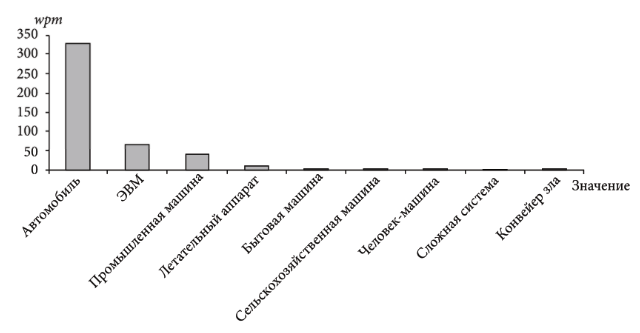
\includegraphics[width=0.8\textwidth]{img/book/mashina/1960-1970}
    \caption{График для слова \textit{машина} для 1960-1970 согласно~\cite{TwoCenturies}}
    \label{fig:TwoCenturiesMashina2}
\end{figure}

Тем не менее, в книге обсуждается использование слова в значении ’Поезд, паровоз.’
в досоветский период, а также в значении ’Устройство для работы с информацией, компьютер’,
которые были не были выделены алгоритмом.

Таким образом, алгоритм в целом отражает значения, в которых использовалось
слово \textit{машина}, согласуясь с данными из толкового словаря и историческим исследованием.
Алгоритм выделяет изменение в частотности двух основных значения, но не вывел информацию по менее важным.

\section*{Молодец}

В результате анализа семем лексемы \textit{молодец} в толковых словарях были выделены пять групп значений,
которые можно условно сформулировать следующим образом:

\begin{enumerate}
    \item Молодой, крепкий, статный мужчина.
    (\textit{«Молодой человек, достигший расцвета лет, крепкий и статный.»} в БТС,
    \textit{«Молодой человек, сильный, крепкого сложения.»} в ТСО,  % TODO: Это не отдельное значение? (в примерах Разбойные молодцы. Ловкачи-молодцы.)
    \textit{«обычно мн. Человек, обычно сильный, смелый, бесшабашный.»} в ТСО
    \textit{«Молодцом называют молодого, здорового, привлекательного парня.»} в ТСД)

    \item Удалец, храбрец, герой (в народной словесности).
    (\textit{«Сильный и смелый герой; удалец, храбрец.»} в БТС,
    \textit{«В народной словесности: удалец, храбрец.»} в ТСО)

    \item Похвала, одобрение чьих-либо действий.
    (\textit{«О том, чьи действия вызвали одобрение, удовлетворение у кого-л.»} в БТС,
    \textit{«Выражение похвалы тому, кто делает что-н. хорошо, ловко, умело.»} в ТСО,
    \textit{«Молодцом вы называете того, чьи действия вы одобряете, хвалите.»} в ТСД,
    \textit{«Похвала»} в «Двух веках в двадцати словах»)

    \item Слуга, помощник, служащий.
(\textit{«Служащий»} в «Двух веках в двадцати словах»)

    \item Бандит или приспешник вражеских групп.
(\textit{«Пренебр. =Молодчик (3 зн.: Пособник, приспешник или участник каких-л. реакционных,
вражеских или преступных групп, организаций.).»} в БТС)
\end{enumerate}

%Кроме того, в словарях отмечено употребление слова \textit{молодец} по отношению к женщине в значении похвалы:
%\textit{«Употребление по отношению к женщине»} в «Двух веках в двадцати словах».

\begin{figure}[H]
	\centering
	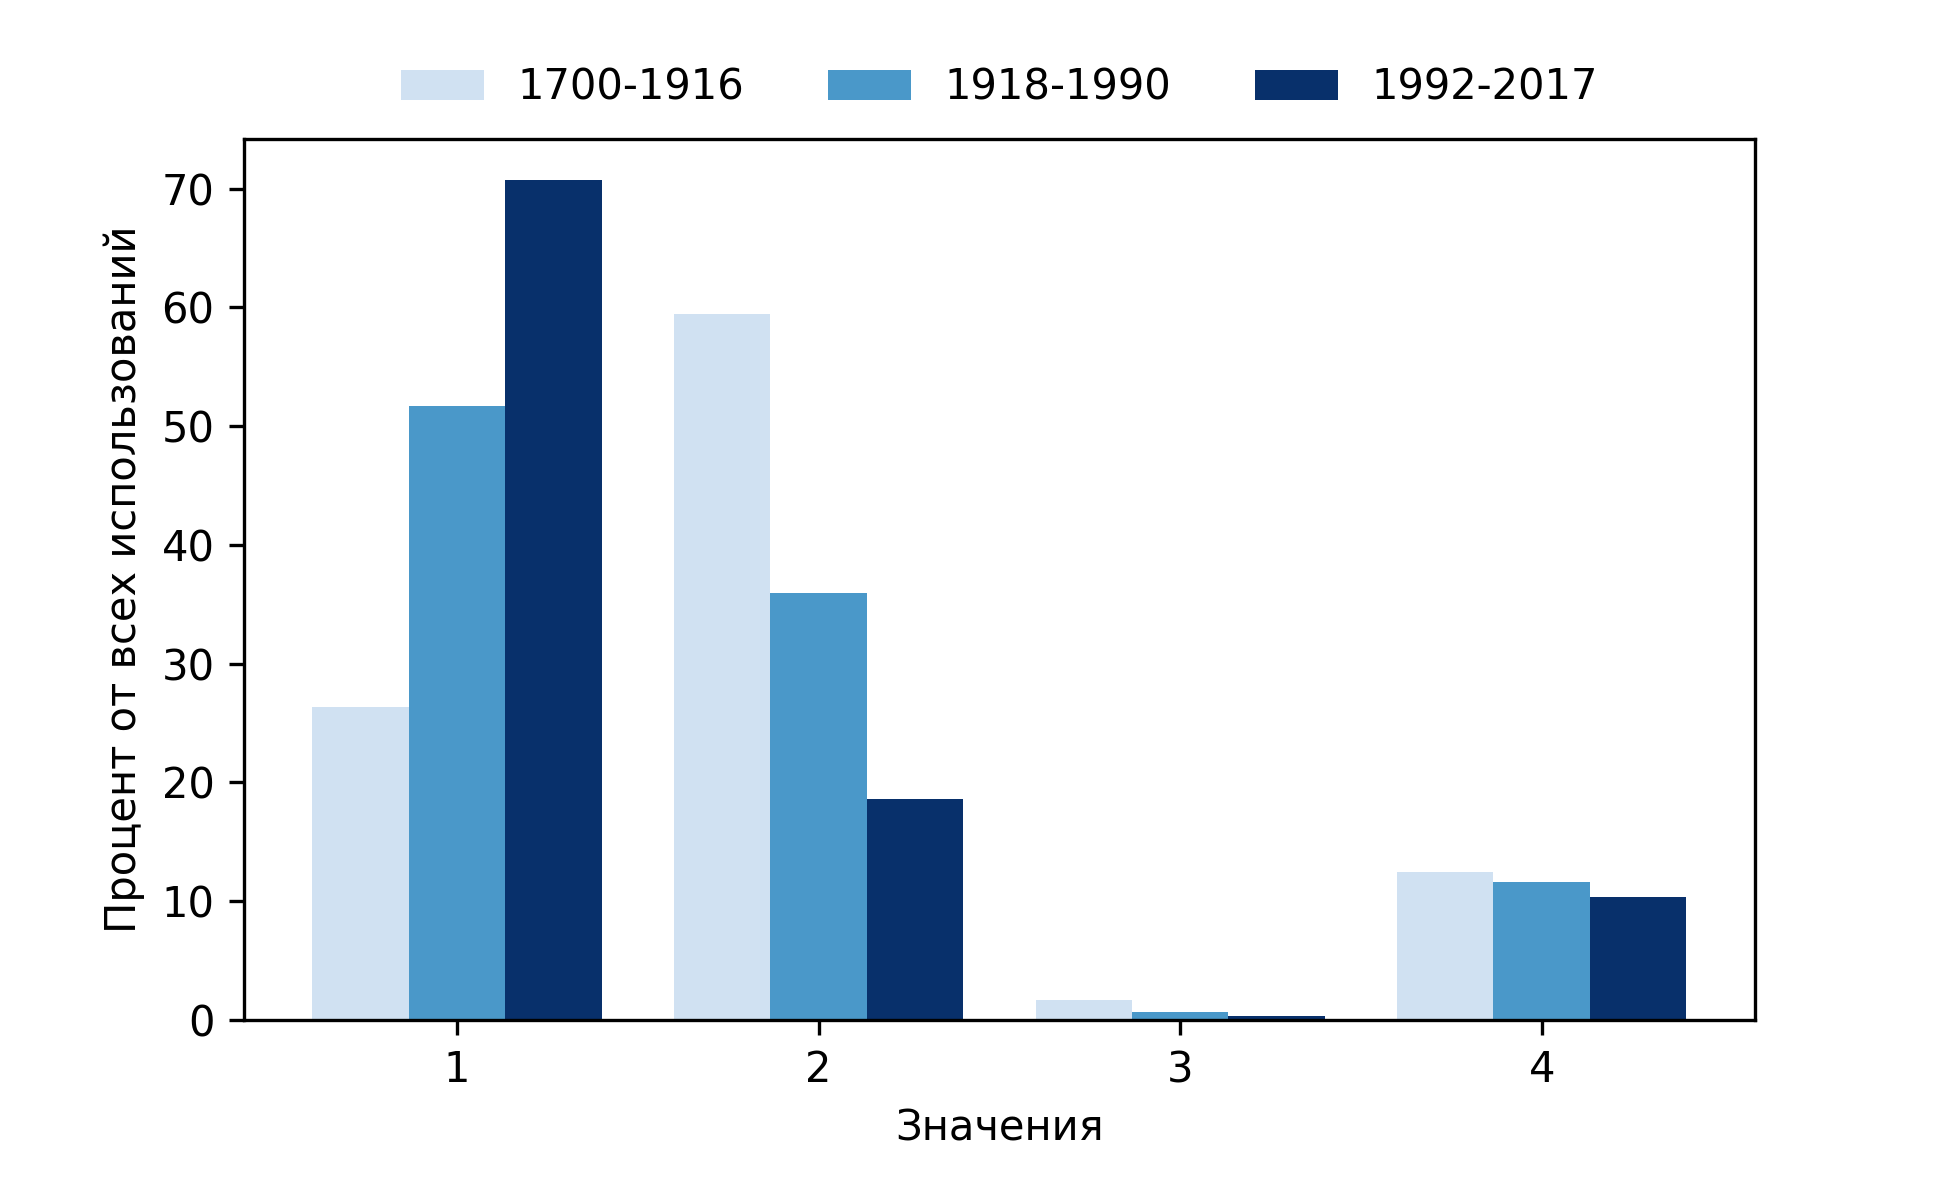
\includegraphics[width=0.8\textwidth]{img/visualizations/molodets_minimal}
	\caption{Изменение значений слова \textit{молодец}}
	\label{fig:Молодец}
\end{figure}

Значения для визуализации слова \textit{Молодец} (Параметры: eps=0.18, min\_samples=10).

\begin{enumerate}
    \item Употребляется как похвала, одобрение.
    \item Молодой человек, юноша.
    \item Употребляется как бранное слово.
    \item О молодом человеке, отличающемся храбростью, удалью и т. п.
\end{enumerate}

\subsection*{Анализ значений слова \textit{молодец}}

Первые четыре определения в визуализации имеют следующие соответствия с обобщенными значениями из словарей:

\begin{itemize}
    \item ’Употребляется как похвала, одобрение.’
Это определение соответствует третьему обобщенному значению:
’Похвала, одобрение чьих-либо действий.’ Общие семы: \textit{’похвала’}, \textit{’одобрение’}. Данный пример является корректным.

    \item ’Молодой человек, юноша.’
    Это определение соответствует первому обобщенному значению:
    ’Молодой, крепкий, статный мужчина.’
    Общие семы: \textit{’молодой’}, \textit{’человек’}.
    Хотя в определении визуализации отсутствуют семы \textit{’крепкий’} и \textit{’статный’}, это определение можно считать корректным, но недостаточно специфичным.

    \item ’Употребляется как бранное слово.’
    Это определение можно считать близким к пятому обобщенному значению:
    ’Бандит или приспешник вражеских групп.’
    Определения объединяет наличие негативной коннотации.
    ’Употребляется как бранное слово.’ определение можно считать имеющим близкое значение,
но не полностью соответствующим,
так как не уточняется денотат.

    \item ’О молодом человеке, отличающемся храбростью, удалью и т. п.’

    Это определение соответствует второму обобщенному значению:
    ’Удалец, храбрец, герой (в народной словесности).’
    Общие семы: \textit{’молодой человек’}, \textit{’храбрость’}, \textit{’удаль’}.
    Это определение можно считать корректным.

\end{itemize}

Обобщённые значения, не найденные в визуализации:

\begin{itemize}
    \item \textbf{Слуга, помощник, служащий.}

    Это значение отсутствует в визуализации.
    Возможно, это значение не достаточно распространено или редко упоминается в используемых данных.
\end{itemize}

\subsection*{Статистика по лексеме \textit{молодец}}
\begin{itemize}
    \item Корректные: 2 (определения 1 и 4)
    \item Недостаточное конкретизирование: 1 (определение 2)
    \item Близкое значение: 1 (определение 3)
\end{itemize}

Таким образом, модель в целом корректно определяет основные значения слова «молодец»,
но не охватывает все возможные значения, представленные в словарях.

Перейдем к частотности значений.

Основным моментом, выделяемым книгой «Два века в двадцати словах», является
выход значения ’Похвала, одобрение чьих-либо действий.’ на лидирующие позиции
вместо изначального значения ’Молодой, крепкий, статный мужчина.’, что можно увидеть
графике~\ref{fig:TwoCenturiesMolodets}.
В визуализации, сделанной алгоритмом, это также отображено.
Значение ’Употребляется как похвала, одобрение.’ растёт с 30\% в досоветский период
растёт до 70\% в постсоветский за счёт уменьшения использования ’Молодой человек, юноша.’.
Также утверждается уменьшение использлвания значения ’Слуга, помощник, служащий.’,
который не был выделен алгоритмом.

\begin{figure}[H]
    \centering % Centers the images
    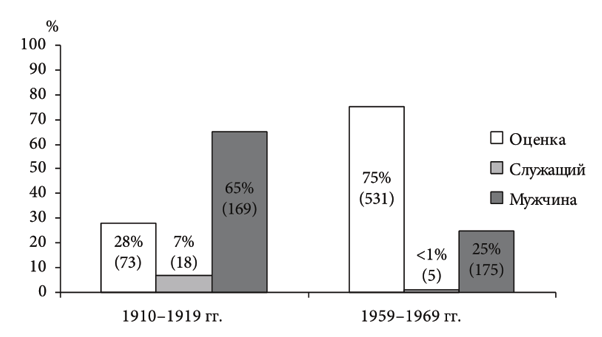
\includegraphics[width=0.8\textwidth]{img/book/molodets/1910-1969}
    \caption{График для слова \textit{молодец} для 1910-1969 согласно~\cite{TwoCenturies}}
    \label{fig:TwoCenturiesMolodets}
\end{figure}

Таким образом, алгоритм в целом отражает значения, в которых использовалось
слово \textit{молодец}, согласуясь с данными из толкового словаря и историческим исследованием.
Алгоритм выделяет основных значения, но не вывел ’Слуга, помощник, служащий.’.

\section*{Передовой}

\begin{enumerate}
    \item Идущий, движущийся впереди остальных; ведущий. \textit{Передовая машина в автоколонне.}
(\textit{«Идущий, движущийся впереди остальных; ведущий.»} в БТС,
\textit{«Движущийся или находящийся впереди.»} в ТСО,
\textit{«Идущий впереди»} в «Двух веках в двадцати словах»)

    \item Находящийся, действующий впереди, в авангарде (о военных силах). \textit{Передовой отряд.}
(\textit{«Находящийся, действующий впереди, в авангарде (о военных силах).»} в БТС,
\textit{«В военном деле передовыми называют отряды, позиции и т. д., находящиеся ближе всего к месту боевых действий.»} в ТСД,
\textit{«Расположенный в авангарде» (о военных действиях)} в «Двух веках в двадцати словах»)

    \item Превосходящий других по уровню своего технического развития. \textit{Передовые достижения в освоении моря.}
(\textit{«Превосходящий других по уровню своего развития; прогрессивный.»} в БТС,
\textit{«Не останавливающийся в развитии, прогрессивный.»} в ТСО,
\textit{«Передовыми называют очень современные, сложные и интересные методы, технологии и т. д.»} в ТСД)

    \item Содержащий, излагающий прогресивные идеи, часто свободолюбивые, либеральные или демократические мысли. \textit{Передовые взгляды.}
(\textit{«Содержащий, излагающий свободолюбивые, либеральные мысли; демократический.»} в БТС,
\textit{«Прогрессивный»} в «Двух веках в двадцати словах»)

    \item Руководящая статья в газете, журнале, печатаемая на первом месте. \textit{Прочитайте передовую.}
(\textit{«Руководящая редакционная статья в газете, журнале, печатаемая на первом месте.»} в ТСО,
\textit{«Статья»} в «Двух веках в двадцати словах»)

    \item Превосходивший других по своим успехам в работе или опережавший других по производственным показателям. \textit{Колхоз, отстававший в прошлые годы по всем показателям, теперь выходит в передовые.}
(\textit{«В СССР: превосходивший других по своим успехам в работе или опережавший других по производственным показателям.»} в БТС,
\textit{«Передовым называли (во времена СССР) человека, коллектив и т. д., который достиг наибольших успехов в работе.»} в ТСД)

    \item Идеи, книги, способствующие какому-то развитию общества, науки, литературы. \textit{Фильм, передовой для своего времени, сейчас безнадёжно устарел.}
(\textit{«Передовыми называют новые современные идеи, книги, способствующие какому-то развитию общества, науки, литературы и т. п.»} в ТСД)

    \item Человек, отправленный для передачи информации или выполнения определенной миссии; посланник, гонец. \textit{Послал передовым.}
(\textit{«Посланник, гонец»} в «Двух веках в двадцати словах»)
\end{enumerate}

\begin{figure}[H]
	\centering
	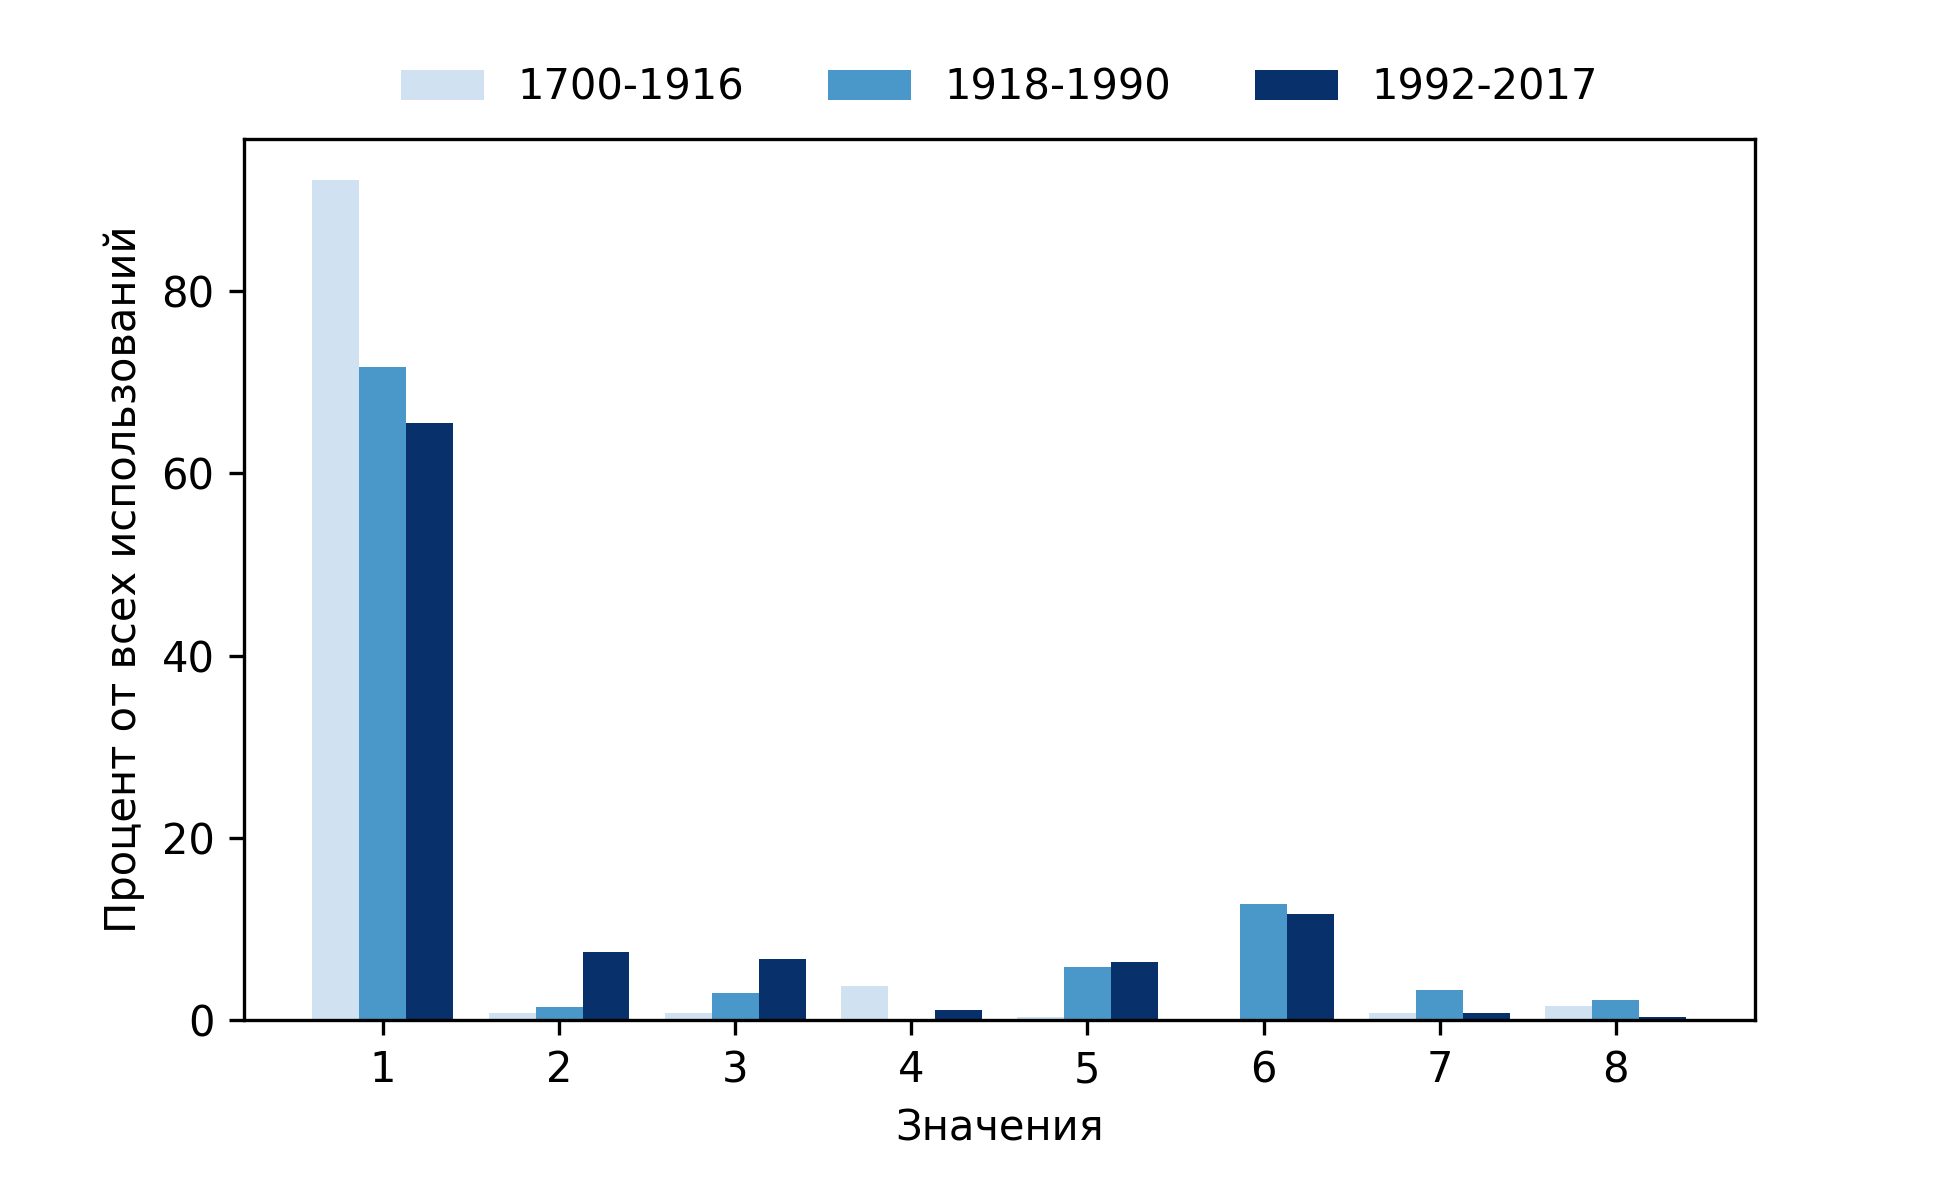
\includegraphics[width=0.8\textwidth]{img/visualizations/peredovoj_minimal}
	\caption{Изменение значений слова \textit{передовой}}
	\label{fig:Передовой}
\end{figure}

Значения для визуализации слова \textit{Передовой} (Параметры: eps=0.18, min\_samples=12).

\begin{enumerate}
    \item Находящийся в авангарде, в первых рядах чего-либо.
    \item Основанный на новейших достижениях науки, техники и т. п.
    \item Содержащий в себе новое, прогрессивное.
    \item Являющийся передовицей.
    \item Передний край обороны, боевых действий.
    \item Передний край, линия фронта.
    \item Главная, основная часть газеты, журнала.
    \item Находящийся на более высокой ступени общественного развития по сравнению с другими.
\end{enumerate}

\subsection*{Анализ значений слова \textit{передовой}}

Первое и четвертое определения корректно сформулированы.
Второе и пятое определения не соответствуют обобщенным значениям.

\begin{itemize}
    \item ’Находящийся в авангарде, в первых рядах чего-либо.’ имеет общий смысловой элемент с
’Идущий, движущийся впереди остальных; ведущий.’,
а именно семы \textit{’находящийся’}, \textit{’в авангарде/в первых рядах’}.

    \item ’Основанный на новейших достижениях науки, техники и т. п.’ полностью соответствует
’Превосходящий других по уровню своего технического развития.’,
так как включает те же семы \textit{’новейшие достижения’}, \textit{’наука, техника’}.

    \item ’Содержащий в себе новое, прогрессивное.’ имеет общий смысловой элемент с
’Содержащий, излагающий прогрессивные идеи, часто свободолюбивые, либеральные или демократические мысли.’,
а именно семы \textit{’содержащий’}, \textit{’новое/прогрессивное’}, однако представляет собой более широкое
определение, так как не ограничивается только идеями.

    \item ’Являющийся передовицей.’ и ’Главная, основная часть газеты, журнала.’ полностью соответствуют
’Руководящая статья в газете, журнале, печатаемая на первом месте.’, так как семы \textit{’главная/основная’}, \textit{’часть газеты, журнала/статья’} полностью отражают смысл ’руководящая статья’.
\end{itemize}

\begin{itemize}
    \item ’Передний край обороны, боевых действий.’ и ’Передний край, линия фронта.’
вместе имеют частичное соответствие с ’Находящийся, действующий впереди, в авангарде (о военных силах).’,
так как семы \textit{’передний край/в авангарде’}, \textit{’боевых действий/военных сил’} частично отражают смысл «впереди, в авангарде».
Однако, данное определение ближе подходит к значению субстантивированного прилагательного «передовая» –
’Участок оборонительной линии, соприкасающейся с неприятельским фронтом; передовая линия.’.
Например, для контекста \textit{Такое случилось еще раз, потому что отказать во встрече уходящему на передовую,
когда к Москве подступают немцы, было невозможно.} было сгенерировано ’Передний край обороны, боевых действий.’.
Исследуемые определения будут считаться нами как корректные.
\end{itemize}

Обобщённые значения, не найденные в визуализации:
\begin{itemize}
    \item ’Превосходивший других по своим успехам в работе или опережавший других по производственным показателям.’
отсутствует среди предложенных моделью значений.
Можно предположить, что информации из контекста использований недостаточно для отделения этого значения от
’Превосходящий других по уровню своего развития; прогрессивный.’. % TODO: проверить

    \item ’Человек, отправленный для передачи информации или выполнения определенной миссии; посланник, гонец.’ также отсутствует в визуализации.
Однако, модель способна на выделение данного значения.
\end{itemize}

Таким образом, для лексемы \textit{передовой} представлено 7 корректных определений.
Среди ошибок присутствуют:
\begin{itemize}
    \item Недостаточное конкретизирование: 1
\end{itemize}

Перейдем к частотности значений.

В книге лишь значение ’Основанный на новейших достижениях науки, техники и т. п.’
указывается как появивишееся после 1917 года, что подтверждается
в визуализации алгоритма, где оно представлено только в советский и постсоветский период.
Кроме того, указано, что военное значение ’Находящийся в авангарде, в первых рядах чего-либо.’
уступает переносным значениям, акцентирующимся на прогрессивности, чего
не наблюдается в визуализации, сделанной алгоритмом.

Снизу расположены графики из книги «Два века в двадцати словах»
для 1830-1859 гг.~\ref{fig:TwoCenturiesPeredovoj1} и 1930-1939 гг.~\ref{fig:TwoCenturiesPeredovoj2}.

\noindent % Prevents indentation for this line to align the images at the left margin
\begin{figure}[H]
    \centering % Centers the images
    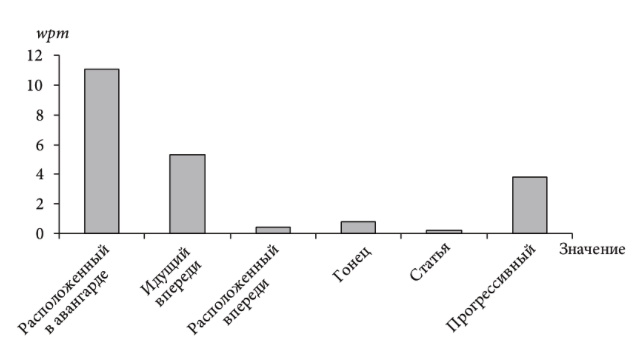
\includegraphics[width=0.8\textwidth]{img/book/peredovoj/1830-1859}
    \caption{График для слова \textit{передовой} для 1830-1859 согласно~\cite{TwoCenturies}}
    \label{fig:TwoCenturiesPeredovoj1}
\end{figure}

\begin{figure}[H]
    \centering % Centers the images
    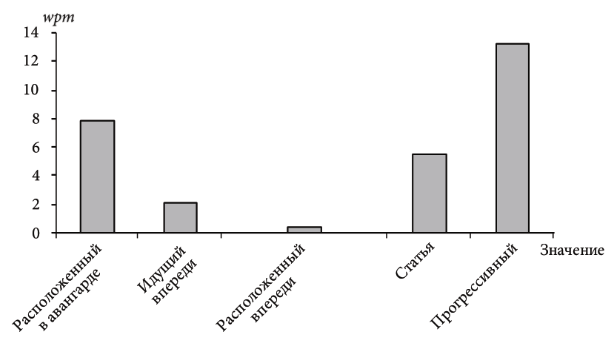
\includegraphics[width=0.8\textwidth]{img/book/peredovoj/1930-1939}
    \caption{График для слова \textit{передовой} для 1930-1939 согласно~\cite{TwoCenturies}}
    \label{fig:TwoCenturiesPeredovoj2}
\end{figure}

Таким образом, нельзя сказать, что алгоритм отражает значения, в которых использовалось
слово \textit{передовой}, так как они не полностью согласуются
с данными из толкового словаря и историческим исследованием.

\section*{Пионер}

\begin{enumerate}
    \item Человек, впервые проникший в неисследованную страну, область и поселившийся в ней. \textit{Пионеры Америки, Сибири, Австралии.}
(\textit{«Человек, впервые проникший в неисследованную страну, область и поселившийся в ней.»} в БТС,
\textit{«Человек, к-рый одним из первых пришел и поселился в новой неисследованной стране, местности.»} в ТСО,
\textit{«Первый поселенец на какой-либо территории»} в «Двух веках в двадцати словах»)

    \item Тот, кто положил начало чему-либо в какой-либо сфере деятельности, в науке, культуре; новатор, зачинатель. \textit{Пионер естествознания.}
(\textit{«Тот, кто прокладывает новые пути в какой-л. сфере деятельности, в науке, культуре; новатор, зачинатель.»} в БТС,
\textit{«Человек, к-рый положил начало чему-н. новому в области науки, культуры »} в ТСО,
\textit{«Первооткрыватель»} в «Двух веках в двадцати словах»)

    \item Член добровольной самодеятельной детской организации. \textit{Вступить, принять в пионеры.}
(\textit{«В СССР: член добровольной самодеятельной детской организации, объединявшей детей и подростков от 10 до 15 лет.»} в БТС,
\textit{«Член детской организации в СССР и ряда детских организаций в нек-рых других странах.»} в ТСО,
\textit{«Член детской организации»} в «Двух веках в двадцати словах»)

    \item Профессия, связанная со строительством мостов и укреплений. \textit{К построению мостов и укреплений посланы прусские инженеры и пионеры.}
(\textit{«Сапер.»} в «Двух веках в двадцати словах»)
\end{enumerate}

\begin{figure}[H]
	\centering
	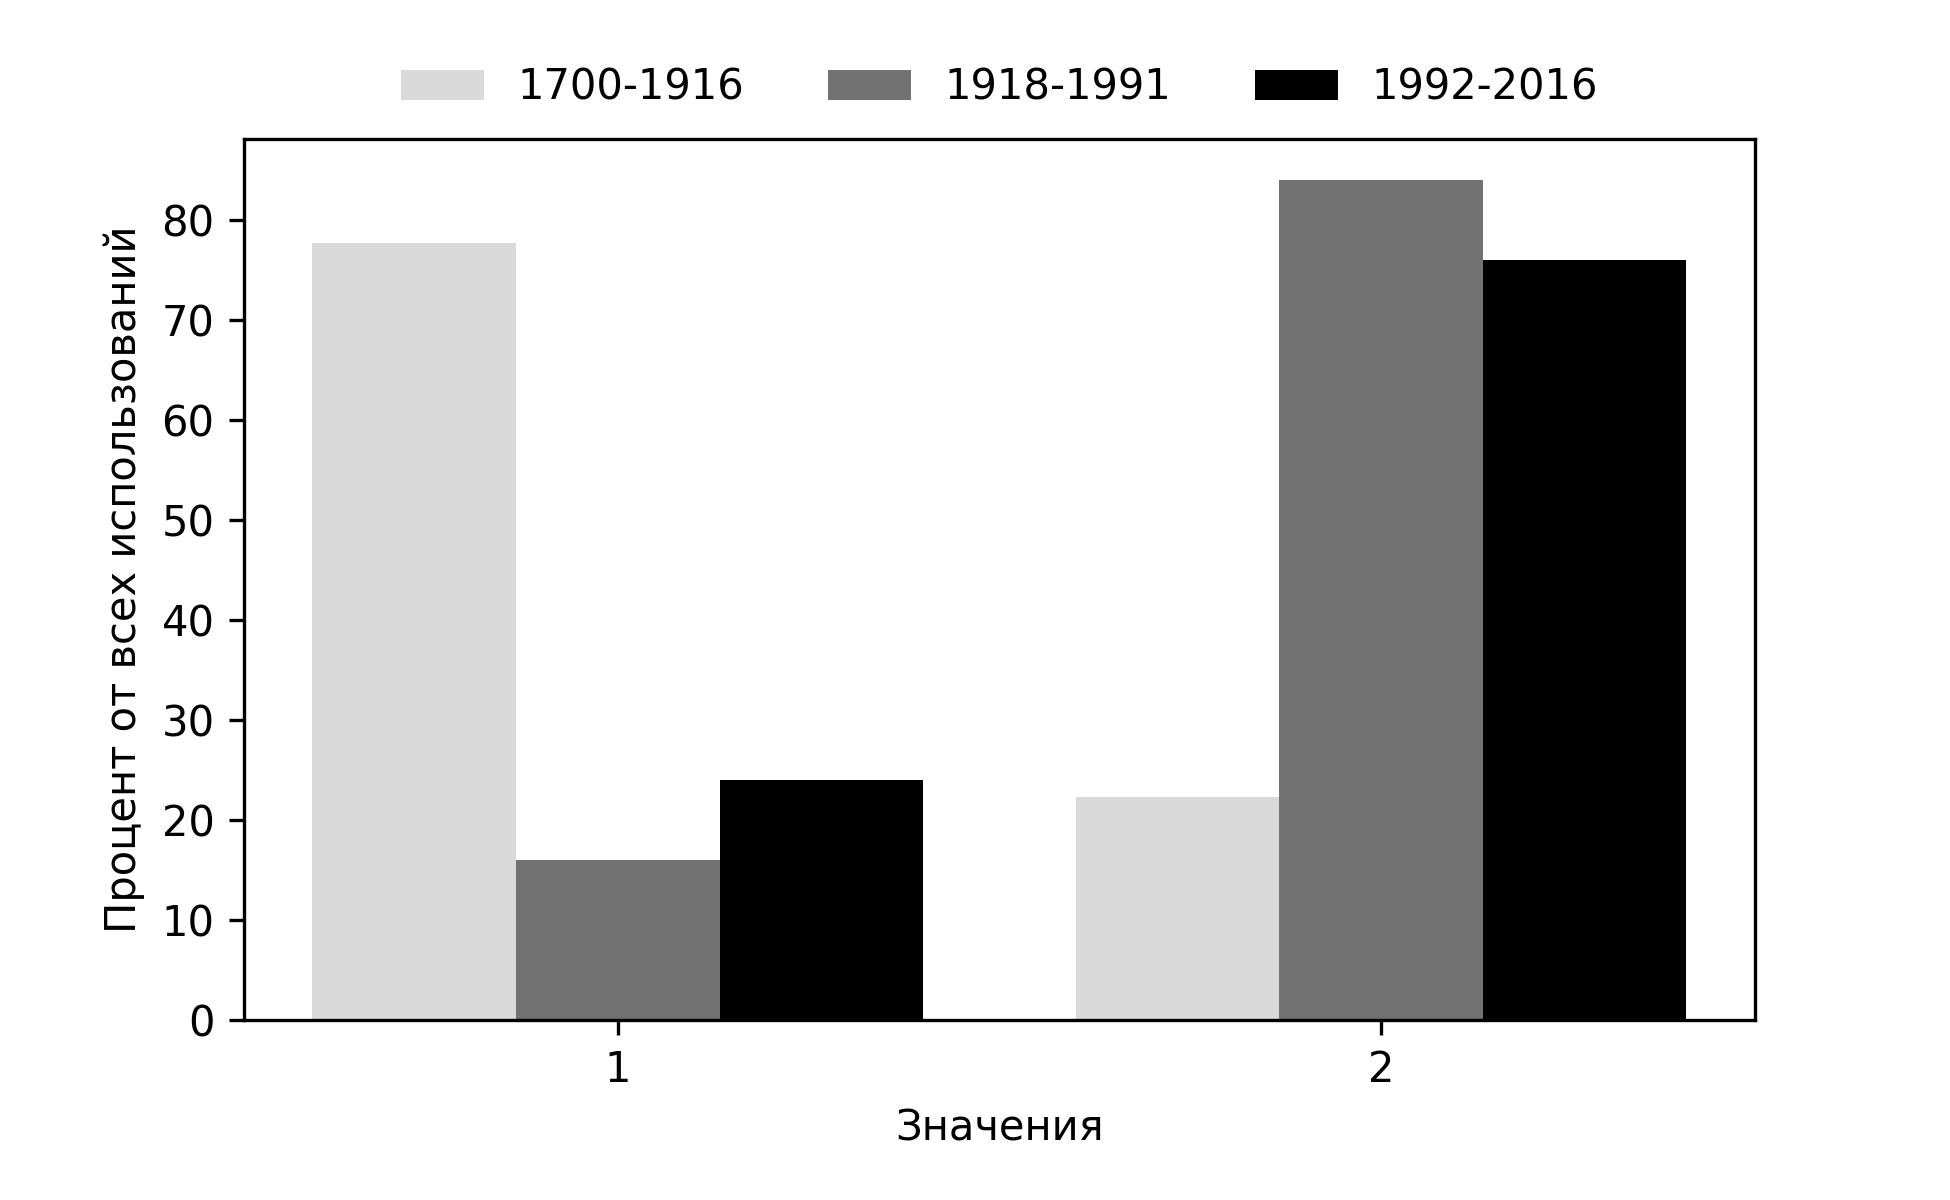
\includegraphics[width=0.8\textwidth]{img/visualizations/pioner_minimal}
	\caption{Изменение значений слова \textit{пионер}}
	\label{fig:Пионер}
\end{figure}

Значения для визуализации слова \textit{пионер} (Параметры: eps=0.18, min\_samples=15).

\begin{enumerate}
    \item Тот, кто первым начал что-либо делать, кто является основоположником чего-либо.
    \item Юный член пионерской организации.
\end{enumerate}

\subsection*{Анализ значений слова \textit{пионер}}

Оба определения корректно сформулированы.

\begin{itemize}
    \item ’Тот, кто первым начал что-либо делать, кто является основоположником чего-либо.’ имеет общий смысловой элемент с
’Тот, кто положил начало чему-либо в какой-либо сфере деятельности, в науке, культуре; новатор, зачинатель.’,
а именно семы \textit{’начало’}, \textit{’деятельность’}, \textit{’новаторство’}.

    \item ’Юный член пионерской организации.’ полностью соответствует
’Член добровольной самодеятельной детской организации.’, так как включает те же семы \textit{’член’}, \textit{’детская организация’}.
\end{itemize}

Обобщённые значения, не найденные в визуализации:
\begin{itemize}
    \item ’Человек, впервые проникший в неисследованную страну, область и поселившийся в ней.’
отсутствует среди предложенных моделью значений.
В книге «Два века в двадцати словах» указывается, что это в русском имело единичные использования.
Можно предположить, что оно не вошло в исследуемую выборку.
Однако, модель способна на выделение данного значения.  % TODO: проверить

    \item ’Профессия, связанная со строительством мостов и укреплений.’ также отсутствует в визуализации.
В книге «Два века в двадцати словах» указывается, что это значение редкое.
Можно предположить, что оно не вошло в исследуемую выборку.
Однако, модель способна на выделение данного значения.  % TODO: проверить
\end{itemize}

Таким образом, для лексемы \textit{пионер} представлено 2 корректных определения.

Перейдем к частотности значений.

Значения, связанные с первооткрывательством, а также с сапёром, появились до 1917 года.
Новым значением является ’Член добровольной самодеятельной детской организации.’,
появившееся в советское время.
В визуализации алгоритма указано около 20\% использований слова в таком значении
в досоветский период, что объясняется двусмысленностью части примеров,
например, «Пионеры слушают это и восхищаются.», где необходим дополнительный контекст
для установления значения.

\begin{figure}[H]
    \centering % Centers the images
    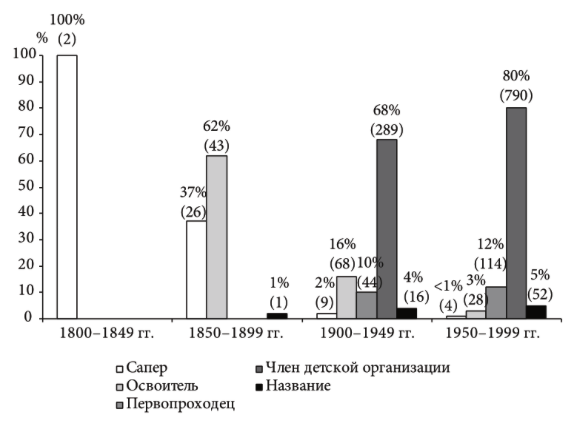
\includegraphics[width=0.8\textwidth]{img/book/pioner/all}
    \caption{График для слова \textit{пионер} согласно~\cite{TwoCenturies}}
\end{figure}

Таким образом, алгоритм лишь частично отражает значения, в которых использовалось
слово \textit{пионер}, так как из 4 значений выделено только 2, из которых
около 20\% размечено неверно.

\section*{Пожалуй}

\begin{enumerate}
    \item Выражение допущения или вероятности. \textit{Было уже, пожалуй, за полночь.}
(\textit{«Вводное слово, выражающее допущение возможного, склонность согласиться.»} в ТСО,
\textit{«Словом пожалуй обозначают вероятность чего-либо.»} в ТСД,
\textit{«Возможно.»} в «Двух веках в двадцати словах»)

    \item Выражение намерения совершить действие. \textit{Я, пожалуй, пойду.}
(\textit{«Слово пожалуй употребляется в том случае, если кто-либо сообщает о своём намерении
совершить какое-либо действие, которое кажется этому человеку наиболее приемлемым в какой-либо ситуации.»} в ТСД,
\textit{«Склоняюсь к тому, что...»} в «Двух веках в двадцати словах»)

    \item Выражение нерешительного, неопределённого согласия. \textit{Чайку не хотите? — Пожалуй.}
(\textit{«Частица, выражающая не уверенное согласие.»} в ТСО,
\textit{«Словом пожалуй обозначают нерешительное, неопределённое согласие что-либо сделать.»} в ТСД,
\textit{«Ладно, согласен.»} в «Двух веках в двадцати словах»)

    \item Вежливое обращение или просьба. \textit{Пожалуй-ка, мой друг, потрудись и поспеши челобитную написать и будь уверен, что я буду тебе благодарен.}
(\textit{«Повелительный наклон, при вежливом обращении.»} в БТС,
\textit{«Будь добр.»} в «Двух веках в двадцати словах»)
\end{enumerate}

\begin{figure}[H]
	\centering
	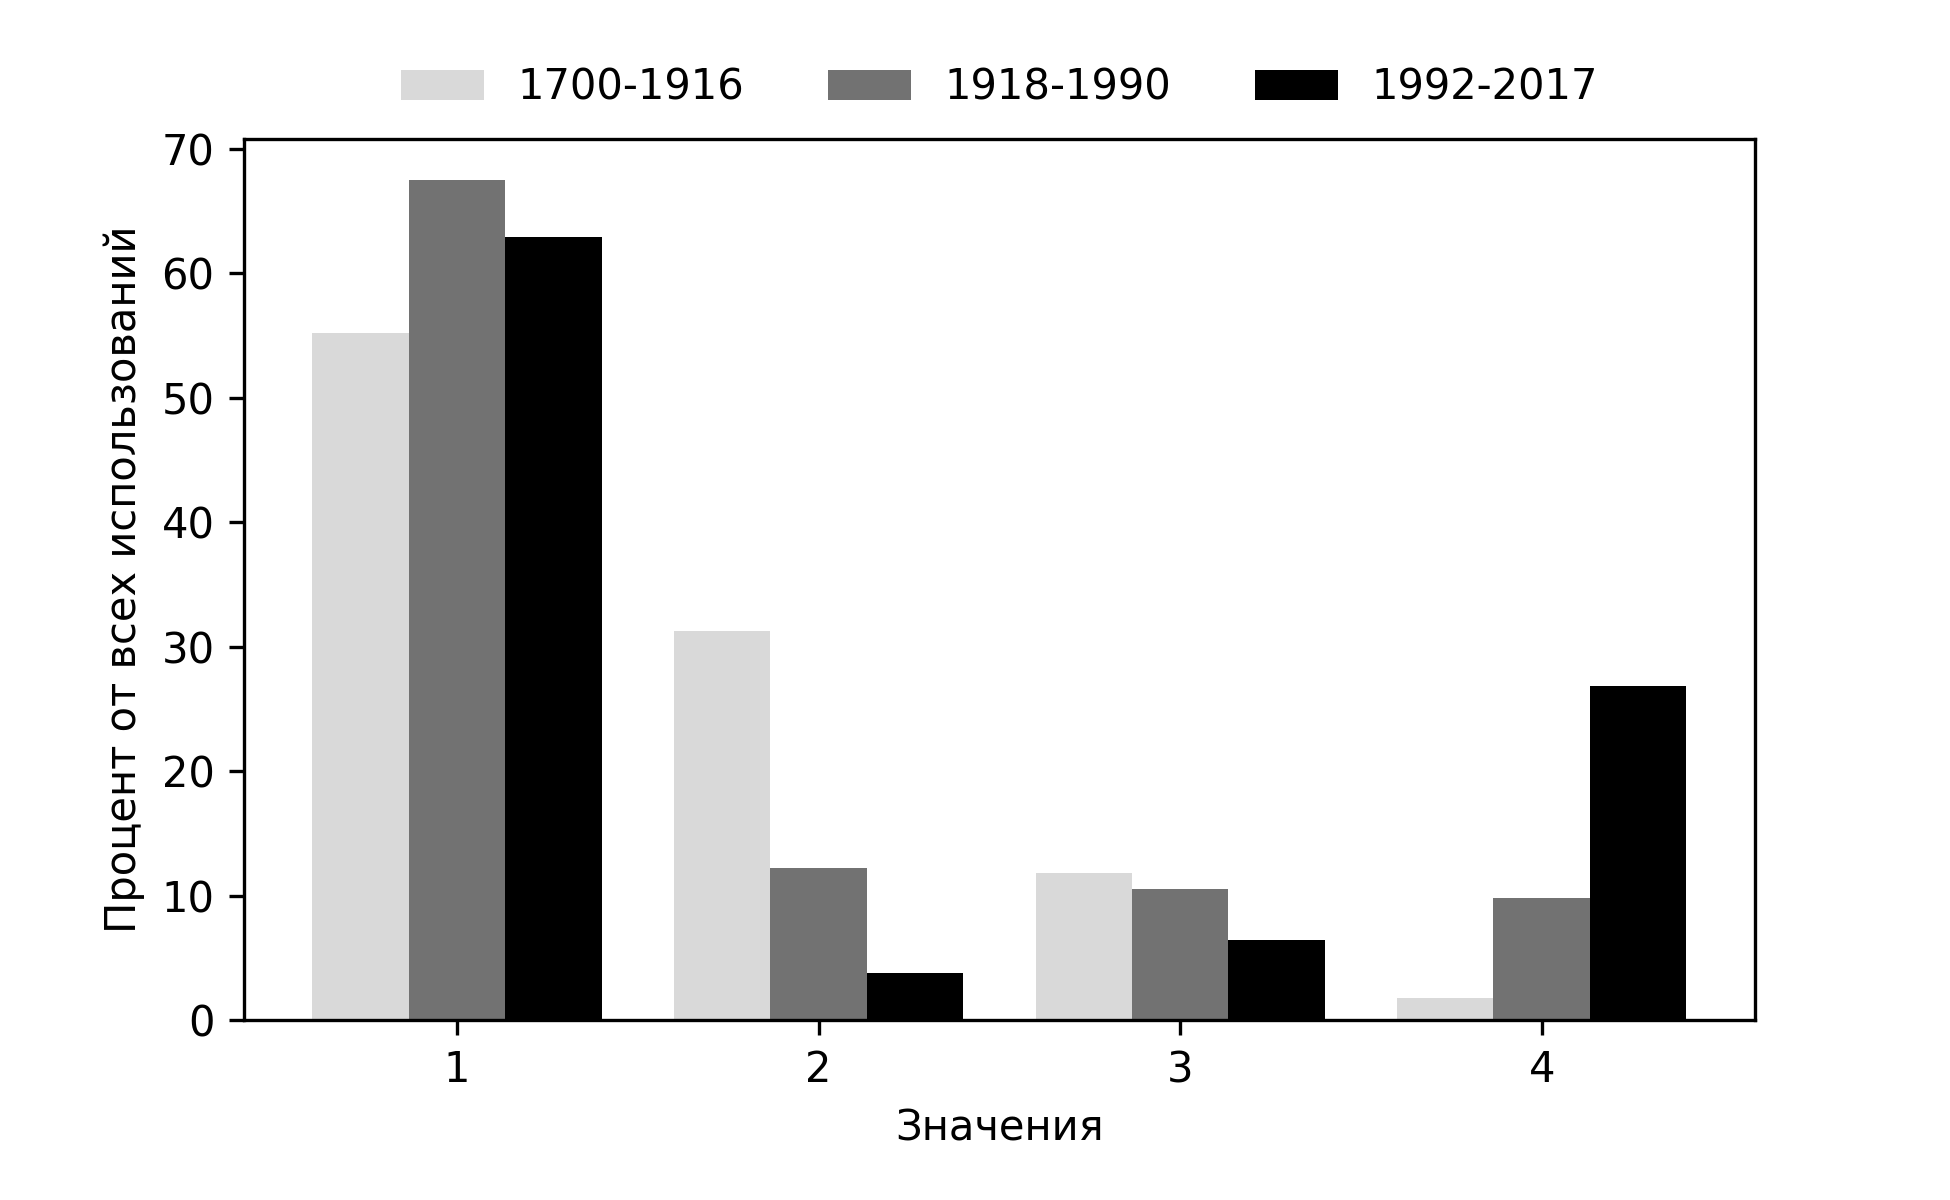
\includegraphics[width=0.8\textwidth]{img/visualizations/pozhaluj_minimal}
	\caption{Изменение значений слова \textit{пожалуй}}
	\label{fig:Пожалуй}
\end{figure}

Значения для визуализации слова \textit{Пожалуй} (Параметры: eps=0.15, min\_samples=10).

\begin{enumerate}
    \item Употребляется для выражения сомнения, неуверенности в чем-либо.
    \item Употребляется для выражения просьбы, приглашения к чему-либо.
    \item Вполне возможно, вероятно.
    \item Употребляется для присоединения предложений или отдельных членов предложений,
усиливающих или уточняющих высказанную мысль.
\end{enumerate}

\subsection*{Анализ значений слова \textit{пожалуй}}

Первое, второе и третье определения корректно сформулированы.
Четвертое определения не соответствуют обобщенным значениям.

\begin{itemize}
    \item ’Употребляется для выражения сомнения, неуверенности в чем-либо.’
не имеет похожих обобщенных определений, а примеры, которые имеют данное определение,
например, \textit{«От отца я, пожалуй, кроме книг ничего в подарок и не получал.»}
было бы корректно отнести к ’Вполне возможно, вероятно.’
%имеет общий смысловой элемент с ’Выражение нерешительного, неопределённого согласия.’,
%а именно семы «сомнение» и «неуверенность», но не имеет семы «согласия».

    \item ’Употребляется для выражения просьбы, приглашения к чему-либо.’ соответствует
’Вежливое обращение или просьба’ с общими семами \textit{’просьбы’}.

    \item ’Вполне возможно, вероятно.’ соответствует
’Выражение допущения или вероятности.’, так как включает те же семы \textit{’возможности’}, \textit{’вероятности’}.
\end{itemize}

\begin{itemize}
    \item ’Употребляется для присоединения предложений или отдельных членов предложений,
усиливающих или уточняющих высказанную мысль.’ является некорректным значением,
так как описывает такое функциональное использование в синтаксисе, что отсутствует в словарях.
\end{itemize}

Обобщённые значения, не найденные в визуализации:
\begin{itemize}
    \item ’Выражение намерения совершить действие’ также отсутствует в визуализации.
Однако, модель способна на выделение данного значения. % TODO: прогнать на примере модель
\end{itemize}

Таким образом, для лексемы \textit{пожалуй} представлено 2 корректных определения.
Среди ошибок присутствуют:
\begin{itemize}
    \item Некорректность определений: 2
\end{itemize}

Перейдем к частотности значений.

В книге сообщается, что изначальные значения ’Вежливое обращение или просьба’
и ’Выражение нерешительного, неопределённого согласия.’ были вытсенены в течение XIX века
преобладающим на сегодняшний момент значением ’Вполне возможно, вероятно.’
В визуализации данная информация подтверждается для значения
’Употребляется для выражения просьбы, приглашения к чему-либо.’,
имевшее в постсовесткий период более 30\% использований и около 5\% в постсовесткий.
Тем не менее, затруднительно установить корректность статистики далее из-за
некорректных определений.

Информация из книги «Два века в двадцати словах» находится на графиках~\ref{fig:TwoCentrutiesPozhaluj1} и~\ref{fig:TwoCentrutiesPozhaluj2}.

\noindent % Prevents indentation for this line to align the images at the left margin
\begin{figure}[H]
    \centering % Centers the images
    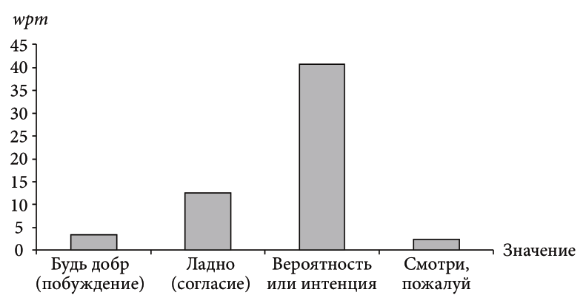
\includegraphics[width=0.8\textwidth]{img/book/pozhaluj/1831-1860}
    \caption{График для слова \textit{пожалуй} для 1831-1860 согласно~\cite{TwoCenturies}}
    \label{fig:TwoCentrutiesPozhaluj1}
\end{figure}

\begin{figure}[H]
    \centering % Centers the images
    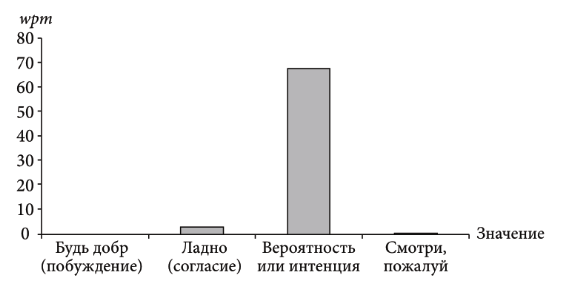
\includegraphics[width=0.8\textwidth]{img/book/pozhaluj/1900-1910}
    \caption{График для слова \textit{пожалуй} для 1900-1910 согласно~\cite{TwoCenturies}}
    \label{fig:TwoCentrutiesPozhaluj2}
\end{figure}

Таким образом, алгоритм лишь частично отражает значения, в которых использовалось
слово \textit{пожалуй}, так как из 4 значений корректны только 2.

\section*{Привет}

\begin{enumerate}
    \item Вежливо-фамильярная форма приветствия при встрече или расставании. \textit{Привет, Алёша, как я рад тебя видеть!}
(\textit{«Дружеское или фамильярное приветствие, обращённое к кому-л. при встрече или расставании.»} в БТС,
\textit{«Приветствие при встрече или расставании.»} в ТСРЯ,
\textit{«Если кто-либо говорит Привет! при встрече с каким-либо человеком или группой людей,
значит, он просто употребляет вежливо-фамильярную форму приветствия.»} в ТСД,
\textit{«Здравствуйте».} в «Двух веках в двадцати словах»)

    \item Обращение к кому-либо с выражением дружеского расположения, дружеских чувств, доброжелательства. \textit{Сердечный, искренний привет.}
(\textit{«Обращённое к кому-л. выражение дружеского расположения, дружеских чувств, доброжелательства.»} в БТС,
\textit{«Обращенное к кому-н. выражение чувства личной приязни, доброго пожелания, солидарности.»} в ТСРЯ,
\textit{«Словесное или несловесное выражение внимания к собеседнику.»} в «Двух веках в двадцати словах»)

    \item Выражение удивления, несогласия, иронии. \textit{Я не понимаю. - Привет, ну, ты даёшь.}
(\textit{«Выражение удивления, несогласия, иронии.»} в БТС,
\textit{«Выражение недоумения, удивленного несогласия.»} в ТСРЯ,
\textit{«Если один человек говорит Привет! другому в ответ на какие-либо
не понравившиеся ему слова или действия, значит, он тем самым выражает удивление, несогласие, иронию.»} в ТСД)

    \item Формула заключения письма с выражением внимания к собеседнику. \textit{Привет от меня всем знакомым в Вашем гарнизоне.}
(\textit{«С приветом, друзья! Ну я ухожу, п.! С дружеским, сердечным, большим и т.п. приветом;
с приветом (заключительная формула письма).»} в БТС,
\textit{«Иногда слова С (большим, пламенным и т. п.) приветом используются в качестве
формально-вежливой заключительной фразы в письме.»} в ТСД,
\textit{«Формула конца письма с выражением внимания к адресату письма.»} в «Двух веках в двадцати словах»)

%    \item Отсутствие ответа или реакции на обращение. \textit{Ни ответа ни привета. }
%(\textit{«Ни ответа ни привета. Об отсутствии ответа, отзыва на чьё-л. обращение, письмо.»} в БТС,
%\textit{«Ни ответа ни привета - нет никакого ответа от кого-н., никаких известий о ком-н.»} в ТСРЯ,
%\textit{«Говоря, что от кого-либо не слышно ни ответа, ни привета,
%вы подразумеваете под этим долгое отсутствие какого-либо отклика со стороны этого человека
%на ваше обращение, письмо.»} в ТСД)

%    \item Описание состояния человека, ведущего себя странно или глуповато.
%(\textit{«С приветом, в зн. прил. Разг. Со странностями, глуповатый или не совсем нормальный (о человеке).»} в БТС,
%\textit{«С приветом кто (прост.) - со странностями, не совсем нормален.»} в ТСРЯ,
%\textit{«Если вы говорите, что кто-либо (совсем) с приветом!, вы в грубоватой или ироничной форме
%выражаете своё мнение о том, что этот человек — со странностями, глуповат или не совсем нормален,
%или ведёт себя таким образом в данной ситуации.»} в ТСД)

    \item Формула выражения внимания к третьему лицу. \textit{Привет от меня всем знакомым в Вашем гарнизоне.}
(\textit{«Формула конца письма с выражением внимания к третьему лицу.»} в «Двух веках в двадцати словах»)

    \item Дружелюбное, ласковое обращение с кем-либо. \textit{С начала владения моего крестьянами положил себе правило, чтоб с ними обращаться простосердечно и откровенно, веселым видом, больше ласковостью и приветом.}
(\textit{Дружелюбное, ласковое обращение с кем-либо.} в «Двух веках в двадцати словах»)
\end{enumerate}

\begin{figure}[H]
	\centering
	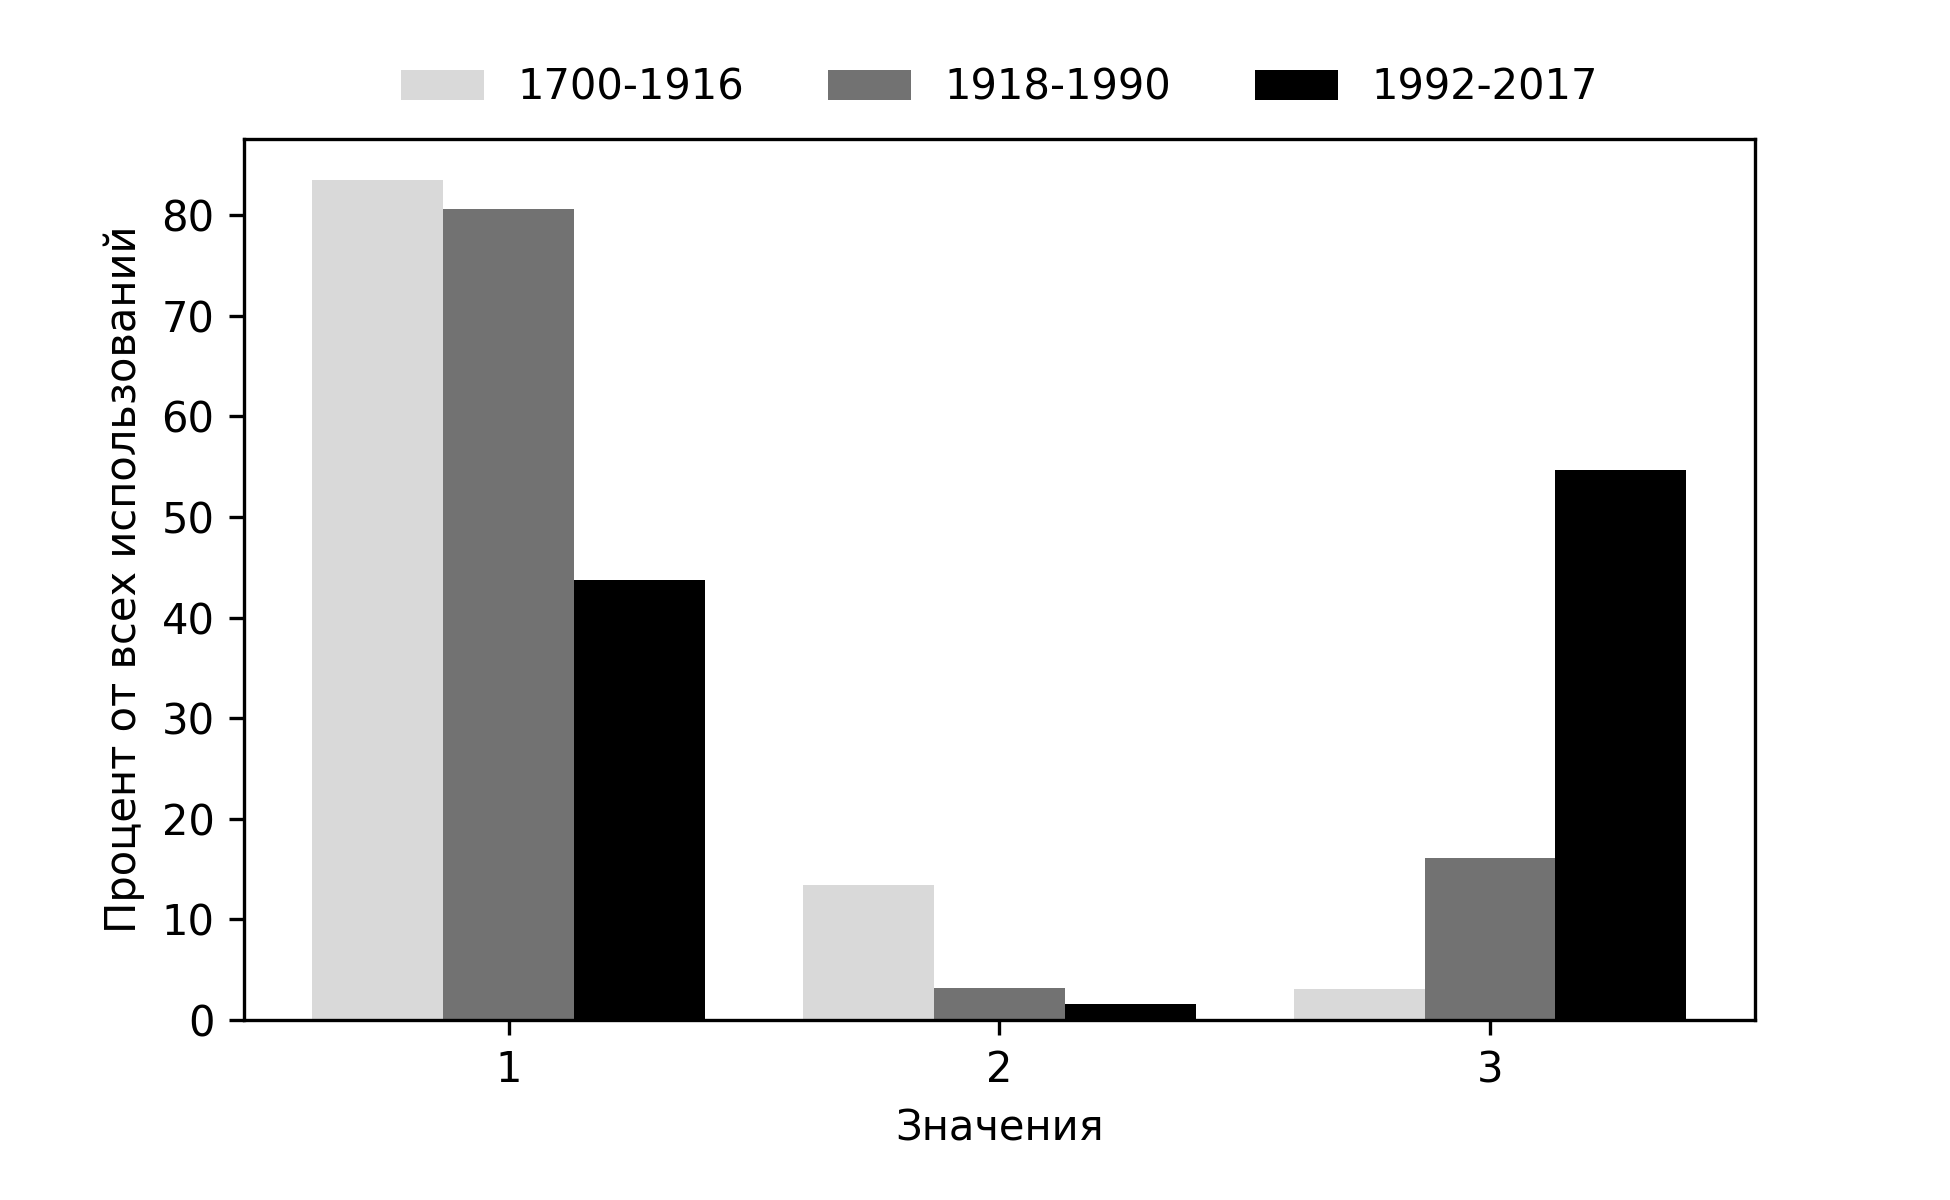
\includegraphics[width=0.8\textwidth]{img/visualizations/privet_minimal}
	\caption{Изменение значений слова \textit{привет}}
	\label{fig:Привет}
\end{figure}

Значения для визуализации слова \textit{привет} (Параметры: eps=0.1, min\_samples=20).

\begin{enumerate}
    \item Устное или письменное обращение к кому-либо с пожеланием доброго здоровья, счастья, успехов и т. п.
    \item Доброжелательное отношение к кому-, чему-либо.
    \item Добрый день, доброе утро.
\end{enumerate}

\subsection*{Анализ значений слова \textit{привет}}

Первое и третье определения корректно сформулированы.
Второе определение имеет обобщенное значение и соответствует конкретным значениям из словарей.

\begin{itemize}
    \item ’Устное или письменное обращение к кому-либо с пожеланием доброго здоровья, счастья, успехов и т. п.’
имеет общий смысловой элемент с ’Обращение к кому-либо с выражением дружеского расположения,
дружеских чувств, доброжелательства.’, а именно семы \textit{’обращение’} и \textit{’доброжелательность’}.

    \item ’Доброжелательное отношение к кому-, чему-либо.’ соответствует значению
’Дружелюбное, ласковое обращение с кем-либо.’,
так как включает те же семы \textit{’доброжелательность/дружелюбность’} и \textit{’отношение/обращение’}.

    \item ’Добрый день, доброе утро.’ соответствует значению
’Вежливо-фамильярная форма приветствия при встрече или расставании.’,
так как представляет из себя синонимичный ряд форм приветствия при встрече.
\end{itemize}

Обобщённые значения, не найденные в визуализации:
\begin{itemize}
    \item ’Выражение удивления, несогласия, иронии.’ отсутствует среди предложенных моделью значений.
    Можно предположить, что информации из контекста использований недостаточно для отделения
    этого значения от общего «доброжелательного обращения».

    \item ’Формула заключения письма с выражением внимания к собеседнику.’ и ’Формула выражения внимания к третьему лицу.’ также отсутствуют в визуализации.
    Однако, модель способна на выделение данных значений при более детализированном контексте.

%    \item ’Отсутствие ответа или реакции на обращение.’ отсутствует среди предложенных моделью значений.
%    Это может быть связано с недостаточной частотностью данного значения в корпусе данных.
%
%    \item ’Описание состояния человека, ведущего себя странно или глуповато.’ также отсутствует в визуализации.
%    Причиной может быть ограниченность контекста или недостаточная выраженность данной семы в корпусе.
\end{itemize}

Таким образом, для лексемы \textit{привет} представлено 3 корректных определения:

Перейдем к частотности значений.

Судя по книге «Два века в двадцати словах» (график снизу), изначальные использования слова \textit{привет}
имели значения ’Обращение к кому-либо с выражением дружеского расположения,
дружеских чувств, доброжелательства.’ и ’Дружелюбное, ласковое обращение с кем-либо.’,
где первое значение было более распространено.
Ближе к завершению советского периода и после на первое место выходит использование
слова \textit{привет} как аналог \textit{здравствуйте}.
Все эти данные подкрепляются в нашей визуализации, где значение ’Добрый день, доброе утро.’
растёт с меньше 5\% в досоветский период до около 55\% в постсоветский, вытесняя
’Устное или письменное обращение к кому-либо с пожеланием доброго здоровья, счастья, успехов и т. п.’
с около 80\% до 45\% и ’Доброжелательное отношение к кому-, чему-либо.’ с 15\% до 2-3\%.
Более того, на графике~\ref{fig:TwoCenturiesPrivet} из книги заметно, что использование ’Доброжелательное отношение к кому-, чему-либо.’
снижается уже в начале советского периода, что так же отражено в нашей визуализации.

\begin{figure}[H]
    \centering % Centers the images
    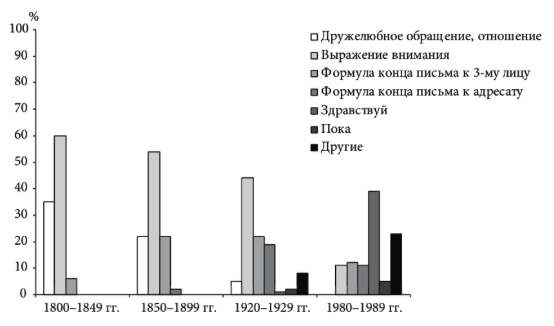
\includegraphics[width=0.8\textwidth]{img/book/privet/all}
    \caption{График для слова \textit{привет} согласно~\cite{TwoCenturies}}
    \label{fig:TwoCenturiesPrivet}
\end{figure}

Таким образом, алгоритм отражает основные значения, в которых использовалось
слово \textit{привет}, согласуясь с данными из толкового словаря и историческим исследованием.

\section*{Пружина}

\begin{enumerate}
    \item Упругая узкая металлическая пластина или нить, согнутая преимущественно в форме спирали. \textit{Пружины матраца, дивана.}
(\textit{«Узкая упругая металлическая пластина или закрученная спиралью металлическая нить
(служащая обычно для приведения в действие механизмов, амортизации ударов и т.п.)»} в БТС,
\textit{«Упругая узкая металлическая пластина или нить, согнутая преимущ. спиралью.»} в ТСО,
\textit{«Он носил маску с железною пружиною, которая не мешала ему есть.»} в «Двух веках в двадцати словах»)

    \item Переносно, движущая сила в каком-то деле. \textit{Главная движущая пружина.}
(\textit{«Движущая сила в каком-н. деле.»} в ТСО, \textit{«Движущая сила чего-л.»} в БТС
\textit{«Природа есть первоначальная всему причина и самодвижущаяся пружина.»} в «Двух веках в двадцати словах»)

    \item Метафора сжатости, а именно, упругость как свойство объекта или субъекта. \textit{Пружины этой души были еще слабы и не расслаблены частым употреблением.}
(\textit{«Метафора сжатости (движения).»} в «Двух веках в двадцати словах»)
\end{enumerate}

\begin{figure}[H]
	\centering
	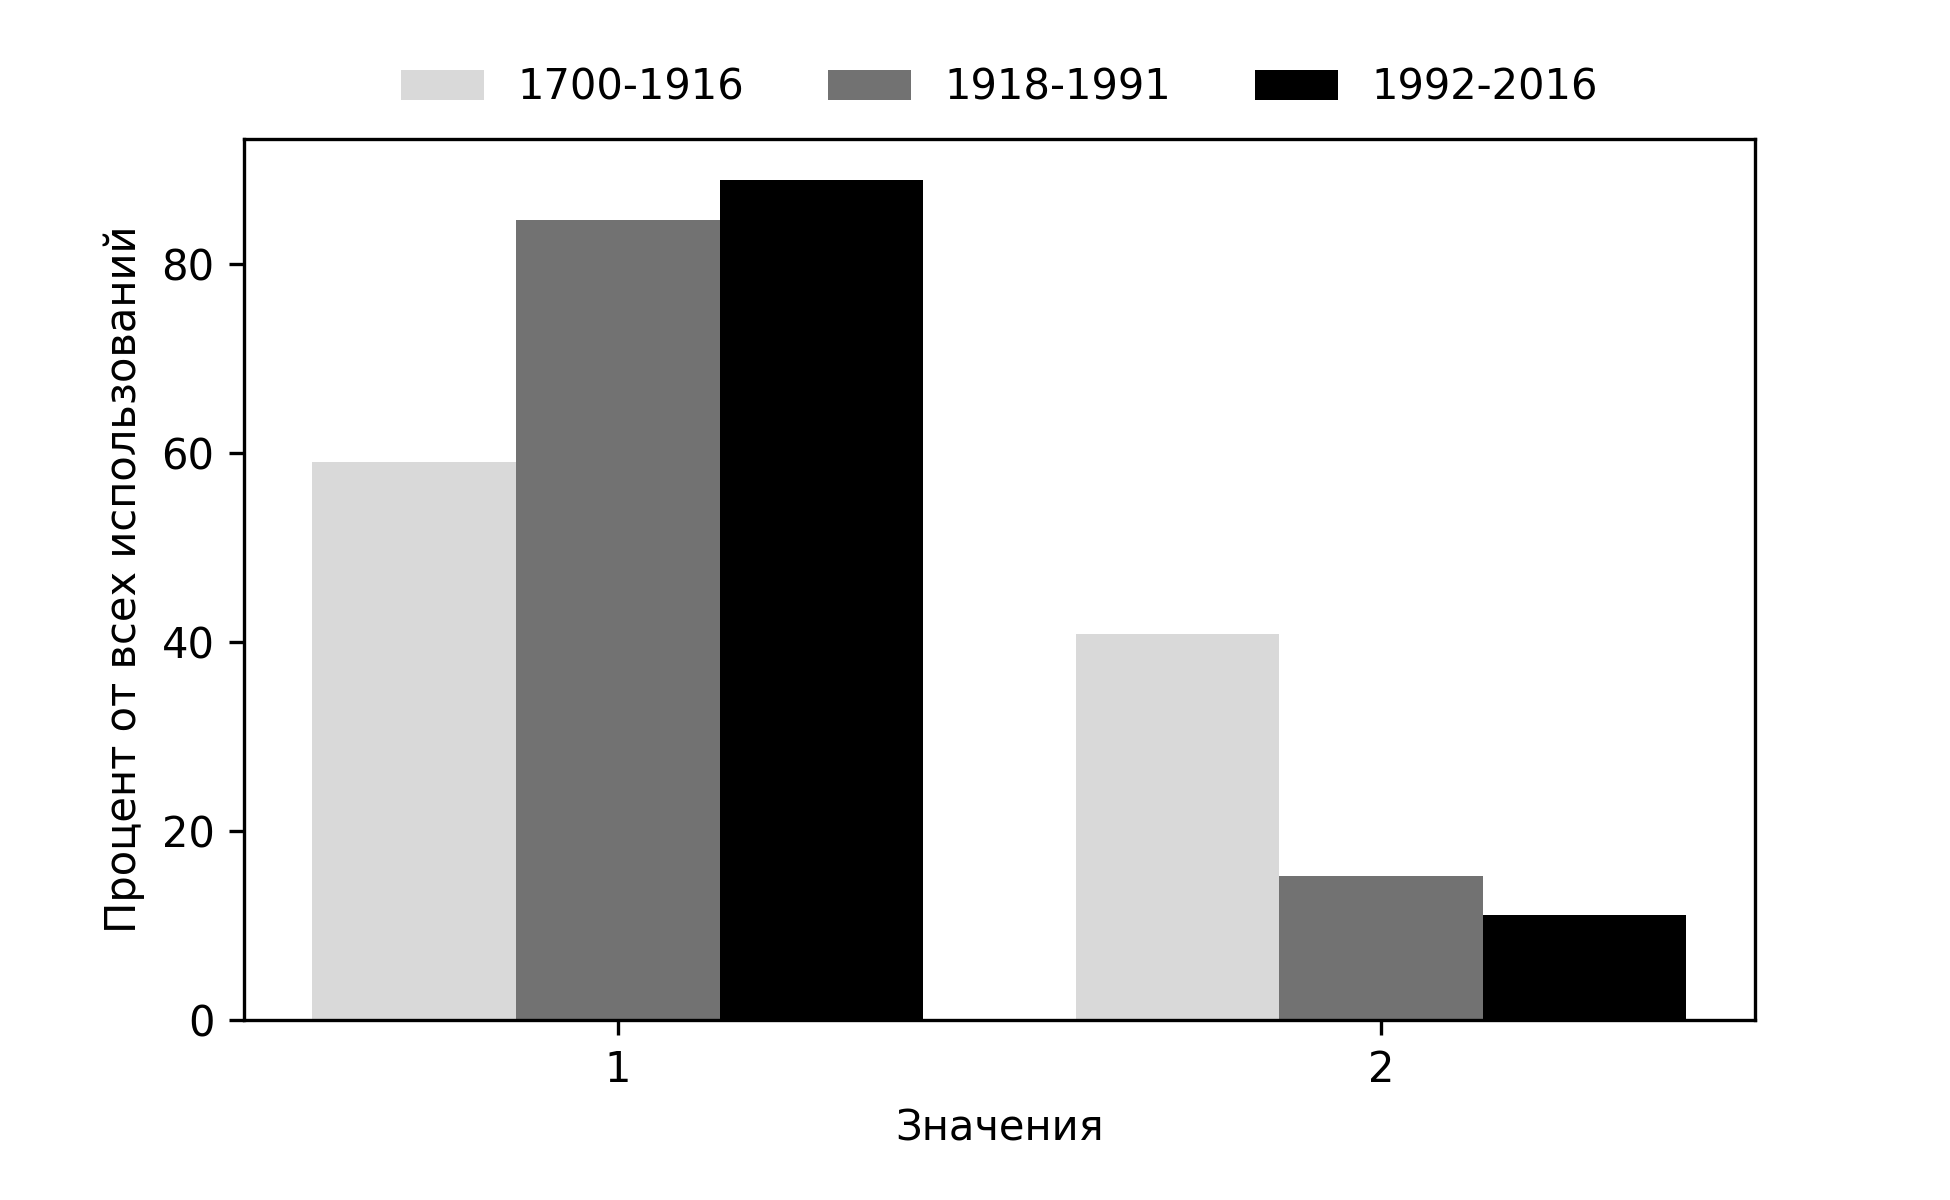
\includegraphics[width=0.8\textwidth]{img/visualizations/pruzhina_minimal}
	\caption{Изменение значений слова \textit{Пружина}}
	\label{fig:Пружина}
\end{figure}

Значения для визуализации слова \textit{Пружина} (Параметры: eps=0.25, min\_samples=50).

\begin{enumerate}
    \item Механизм, приводимый в действие сжатием и разжатием упругого стержня.
    \item То, что является движущей силой, источником чего-либо.
\end{enumerate}

\subsection*{Анализ значений слова \textit{машина}}

Первое и второе определения корректно сформулированы.

\begin{itemize}
    \item ’Механизм, приводимый в действие сжатием и разжатием упругого стержня.’ имеет общий смысловой элемент с
’Упругая узкая металлическая пластина или нить, согнутая преимущественно в форме спирали.’, а именно семы \textit{’механизм’}, \textit{’упругость’}, \textit{’сжатие/разжатие’}, \textit{’стержень’}.

    \item ’То, что является движущей силой, источником чего-либо.’ полностью соответствует
’Переносно, движущая сила в каком-то деле.’, так как включает те же семы \textit{’движущая сила’}, \textit{’источник’}.
\end{itemize}

\begin{itemize}
    \item Метафорическое значение ’Метафора сжатости, а именно, упругость как свойство объекта или субъекта.’ не представлено в визуализации.
Это значение указано только в книге «Два века в двадцати словах» как самое редкое для всех периодов.
Вероятно, оно недостаточно распространено в исследуемом материале, поэтому не вошло в визуализацию.
\end{itemize}

Таким образом, для лексемы \textit{пружина} представлено 2 корректных определения.

Перейдем к частотности значений.

В книге «Два века в двадцати словах» (графики ниже) сообщается о постепенной замене
преобладающего метафорического значения слова (’Переносно, движущая сила в каком-то деле.’)
на прямое (’Упругая узкая металлическая пластина или нить, согнутая преимущественно в форме спирали.’)
в конце XIX века и о нынешнем преобладании прямого значения.
Такие же данные представлены в нашей визуализации, где использования
’То, что является движущей силой, источником чего-либо.’ падают с 40\% до 10\%.

\noindent % Prevents indentation for this line to align the images at the left margin
\begin{figure}[H]
    \centering % Centers the images
    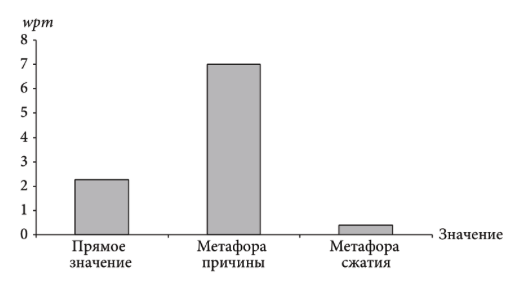
\includegraphics[width=0.8\textwidth]{img/book/pruzhina/1830-1859}
    \caption{График для слова \textit{пружина} для 1830-1859 согласно~\cite{TwoCenturies}}
\end{figure}

\begin{figure}[H]
    \centering % Centers the images
    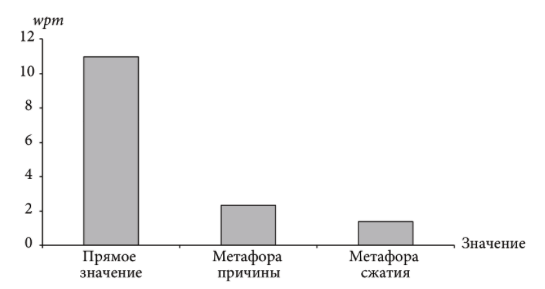
\includegraphics[width=0.8\textwidth]{img/book/pruzhina/1960-2008}
    \caption{График для слова \textit{пружина} для 1960-2008 согласно~\cite{TwoCenturies}}
\end{figure}

Таким образом, алгоритм отражает основные значения, в которых использовалось
слово \textit{пружина}, согласуясь с данными из толкового словаря и историческим исследованием.

\section*{Публика}

В результате анализа семем лексемы \textit{публика} в толковых словарях были выделены следующие группы значений:

\begin{enumerate}
    \item Люди, присутствующие в качестве зрителей, слушателей, посетителей. \textit{Концертная, театральная публика.}
(\textit{«Лица, находящиеся где-либо в качестве посетителей, зрителей, слушателей.»} в БТС,
\textit{«Люди, находящиеся где-нибудь в качестве зрителей, слушателей, пассажиров.»} в ТСО,
\textit{«Публикой называют людей, которые собираются, присутствуют где-либо в качестве зрителей, слушателей.»} в ТСД,
\textit{«Публикой называют людей, которые собираются, присутствуют где-либо в качестве посетителей.»} в ТСД,
\textit{«Аудитория, зрители, слушатели»} в «Двух веках в двадцати словах»)

    \item Люди и общество вообще. \textit{Широкая публика.}
(\textit{«Люди, общество.»} в БТС,
\textit{«Вообще люди, общество.»} в ТСО,
\textit{«Публикой иронично называют категорию людей, которым свойственны какие-либо общие признаки.»} в ТСД)

    \item Группа лиц, объединённые по общим признакам, часто с негативной коннотацией. \textit{Знаю я эту публику - болтуны.}
(\textit{«Неодобрительно о лицах, объединённых по каким-либо признакам.»} в БТС,
\textit{«Общество или отдельные лица, объединённые по каким-н. общим признакам.»} в ТСО,
\textit{«Публикой иронично называют категорию людей, которым свойственны какие-либо общие признаки.»} в ТСД)

    \item Пассажиры, люди в общественном транспорте. \textit{Проголодавшаяся публика бросилась из вагонов в буфет.}
(\textit{«Пассажиры»} в «Двух веках в двадцати словах»,
\textit{«Люди, находящиеся где-нибудь в качестве зрителей, слушателей, пассажиров.»} в ТСО)

    \item Светское общество, привилегированный класс населения. \textit{В Москве всякий всякого по пяти раз на неделю может видеть в публике.}
(\textit{«Светское общество.»} в «Двух веках в двадцати словах»)

    \item Читатели, аудитория, воспринимающая литературные или иные творческие произведения. \textit{Теперь я понимаю, за что В*(яземский) и П*(ушкин] так любят уездных барышен. Они их истинная публика.}
(\textit{«Читатели»} в «Двух веках в двадцати словах»)

    \item Обозримая группа людей. \textit{Капитан тянул баритона, а расстрига спускал октаву, и кабацкая публика находила, что дуэты их выходят весьма чувствительны.}
(\textit{«Народец (обозримая группа людей).»} в «Двух веках в двадцати словах»)

    \item Скопление народа, уличная толпа, масса. \textit{Главные улицы, пассажи и городские ряды кишат публикой, являющейся за по-купками для обнов.}
(\textit{«Уличная толпа, масса.»} в «Двух веках в двадцати словах»)

%    \item Фразеологизмы:
%    \begin{enumerate}
%        \item Работать на публику — делать что-то с целью привлечения внимания и одобрения окружающих.
%        (\textit{«Если кто-либо работает на публику, то это означает, что этот человек делает что-либо с намерением, чтобы его действия были замечены, оценены кем-либо.»} в ТСД)
%    \end{enumerate}
\end{enumerate}

\begin{figure}[H]
	\centering
	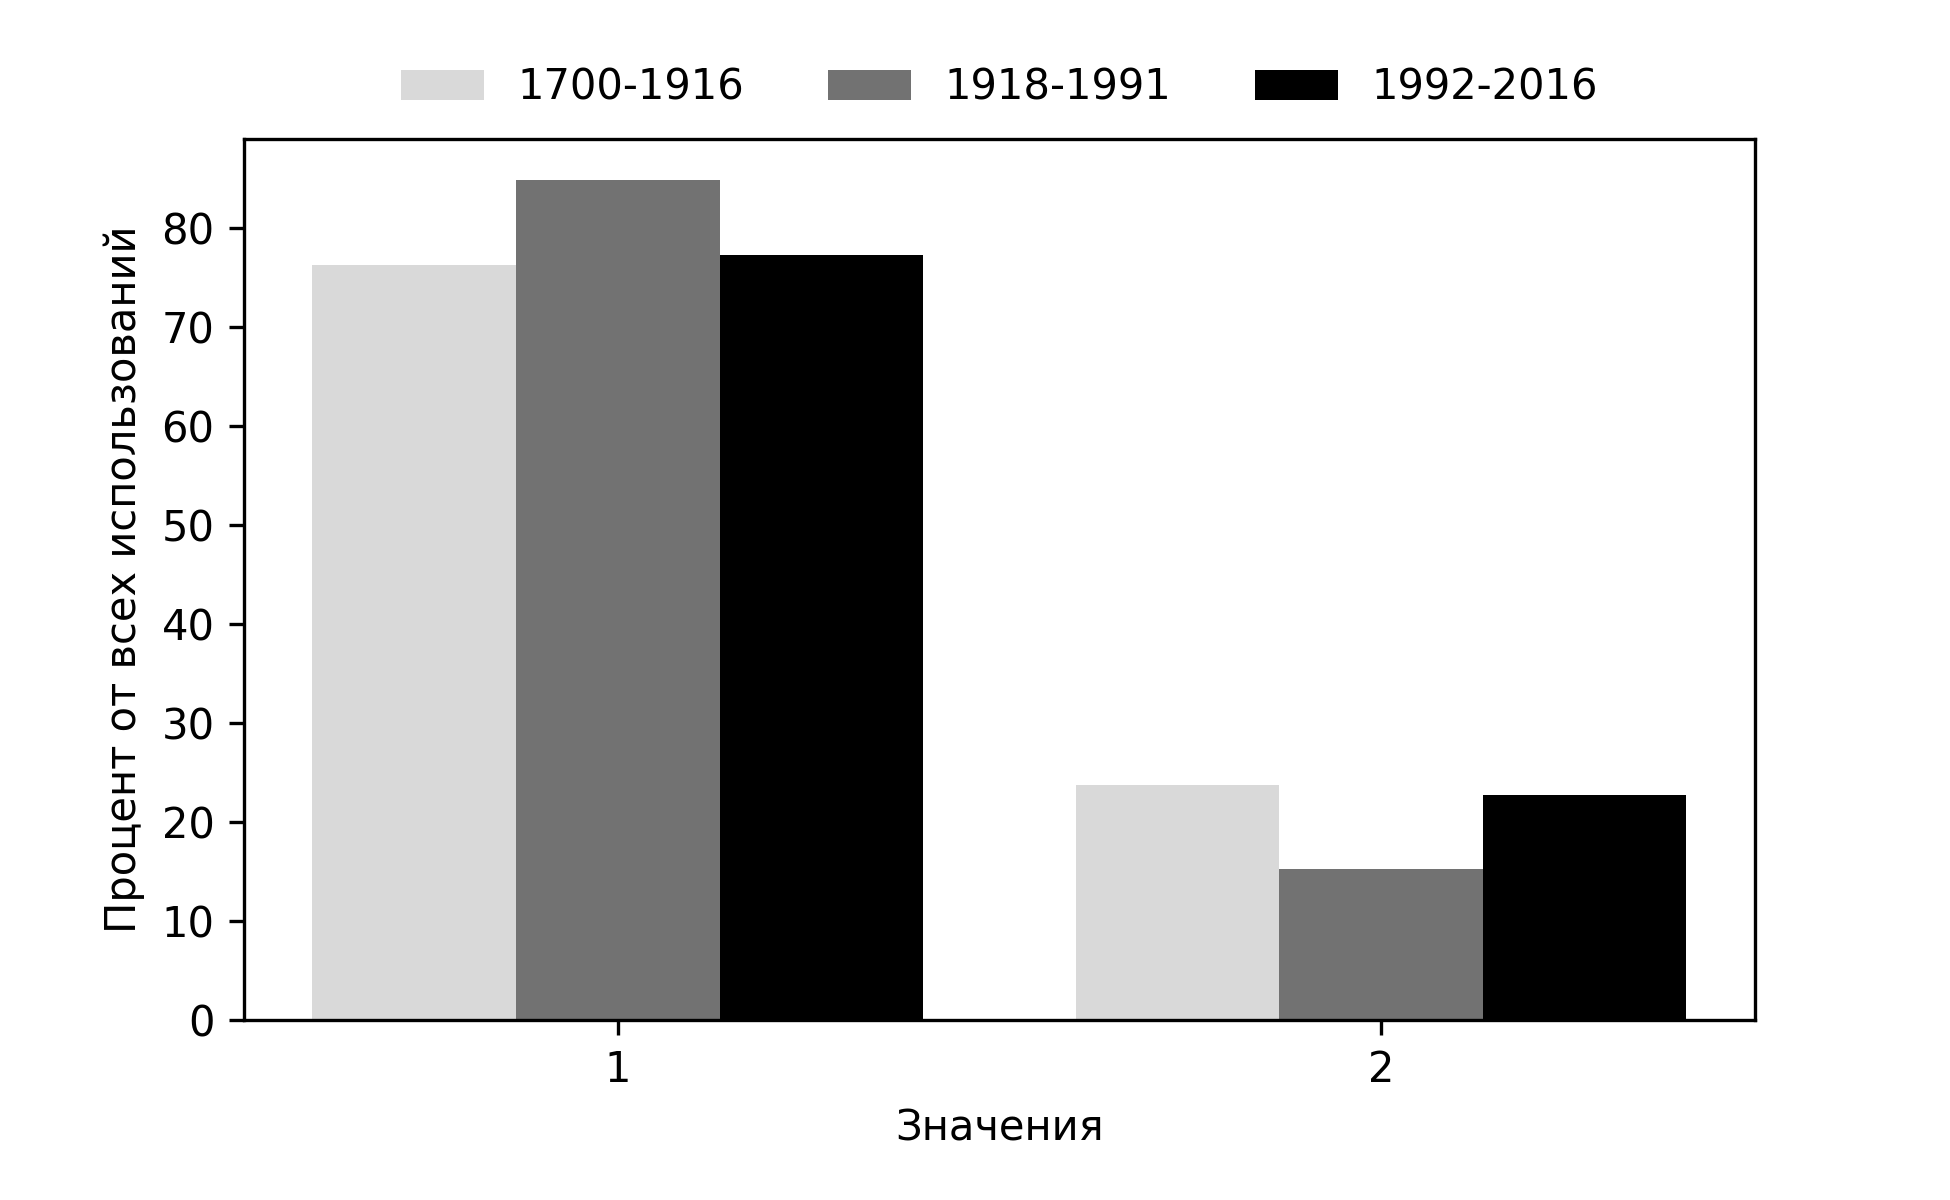
\includegraphics[width=0.8\textwidth]{img/visualizations/publika_minimal}
	\caption{Изменение значений слова \textit{Публика}}
	\label{fig:Публика}
\end{figure}

Значения для визуализации слова «Публика» (Параметры: eps=0.11, min\_samples=10).

\begin{enumerate}
    \item Люди, присутствующие на каком-л. собрании, спектакле, концерте и т. п.
    \item Общество, народ.
\end{enumerate}

\subsection*{Анализ значений слова \textit{публика}}

Оба определения корректно сформулированы.

Оба определения имеют явные аналоги в составленном ранее описании значений слова.

\begin{itemize}
    \item ’Люди, присутствующие на каком-л. собрании, спектакле, концерте и т. п.’ имеет соответствие с
    ’Люди, присутствующие в качестве зрителей, слушателей, посетителей.’.
    Общими смысловыми элементами являются «люди», «присутствующие», «мероприятие».

    \item ’Общество, народ.’ соответствует значению ’Люди и общество вообще.’.
    Общими семами являются «люди», «общество/народ».
\end{itemize}

Не предлагаются следующие значения:
\begin{itemize}
    \item ’Светское общество, привилегированный класс населения.’.
    \item ’Группа лиц, объединённые по общим признакам, часто с негативной коннотацией.’.
    \item ’Пассажиры, люди в общественном транспорте.’.
    \item ’Читатели, аудитория, воспринимающая литературные или иные творческие произведения.’.
    \item ’Обозримая группа людей.’.
    \item ’Скопление народа, уличная толпа, масса.’.
\end{itemize}

Таким образом, для лексемы \textit{публика} представлено 2 корректных определения.

Перейдем к частотности значений.

К сожалению, в книге «Два века в двадцати словах» не даётся
графиков частотности для слова \textit{публика}.
Гооврится лишь о преобладании значения ’аудитория’ и о его оттенках,
которые не удается полноценно сравнить из-за того, что алгоритм предложил довольно общие значения.

\section*{Свалка}

В результате анализа семем лексемы \textit{свалка} в толковых словарях были
выделены семь групп значений, которые можно условно сформулировать
следующим образом:

\begin{enumerate}
    \item Место для сбора мусора, нечистот. \textit{Вывезти мусор на свалку.}
(\textit{«Место, куда свозят, выбрасывают мусор, нечистоты, негодные вещи.»} в БТС,
\textit{«Место, куда вывозят, выбрасывают мусор, нечистоты, негодные вещи.»} в ТСД,
\textit{«Место для сбора мусора, нечистот»} в «Двух веках в двадцати словах»)
    \item Груда, куча, нагромождение чего-либо. \textit{Вывезти мусор на свалку.}
(\textit{«Беспорядочно накиданная груда, куча чего-л.»} и
\textit{«Если кто-либо превращает квартиру в свалку, то это означает, что там в беспорядке нагромождаются предметы, мебель и пр.»} в БТС,
\textit{«Свалкой называют беспорядочно накиданную груду каких-либо предметов.»} в ТСД,
\textit{«Груда»} в «Двух веках в двадцати словах»)
    \item Процесс сваливания. \textit{Свалка песка с платформы.}
(\textit{«к Свалить»} в БТС,
\textit{«Процесс сваливания»} в «Двух веках в двадцати словах»)
    \item Всеобщая драка. \textit{Вмешаться в свалку.}
(\textit{«Свалкой называют всеобщую драку, в которой участвует много людей»} в ТСД,
\textit{«Драка»} в «Двух веках в двадцати словах»)
    \item Скопление людей, толпа. \textit{Людская свалка.}
(\textit{«Скопление людей, толпа.»} в «Двух веках в двадцати словах» и в БТС)
    \item Вооруженное столкновение войск, битва. \textit{В жару свалки они в разных местах расстроили нашу линию, и человек 20 баварцев вдруг прорвались сквозь наш фронт.}
(\textit{«Битва»} в «Двух веках в двадцати словах»)
\end{enumerate}

\begin{figure}[H]
	\centering
	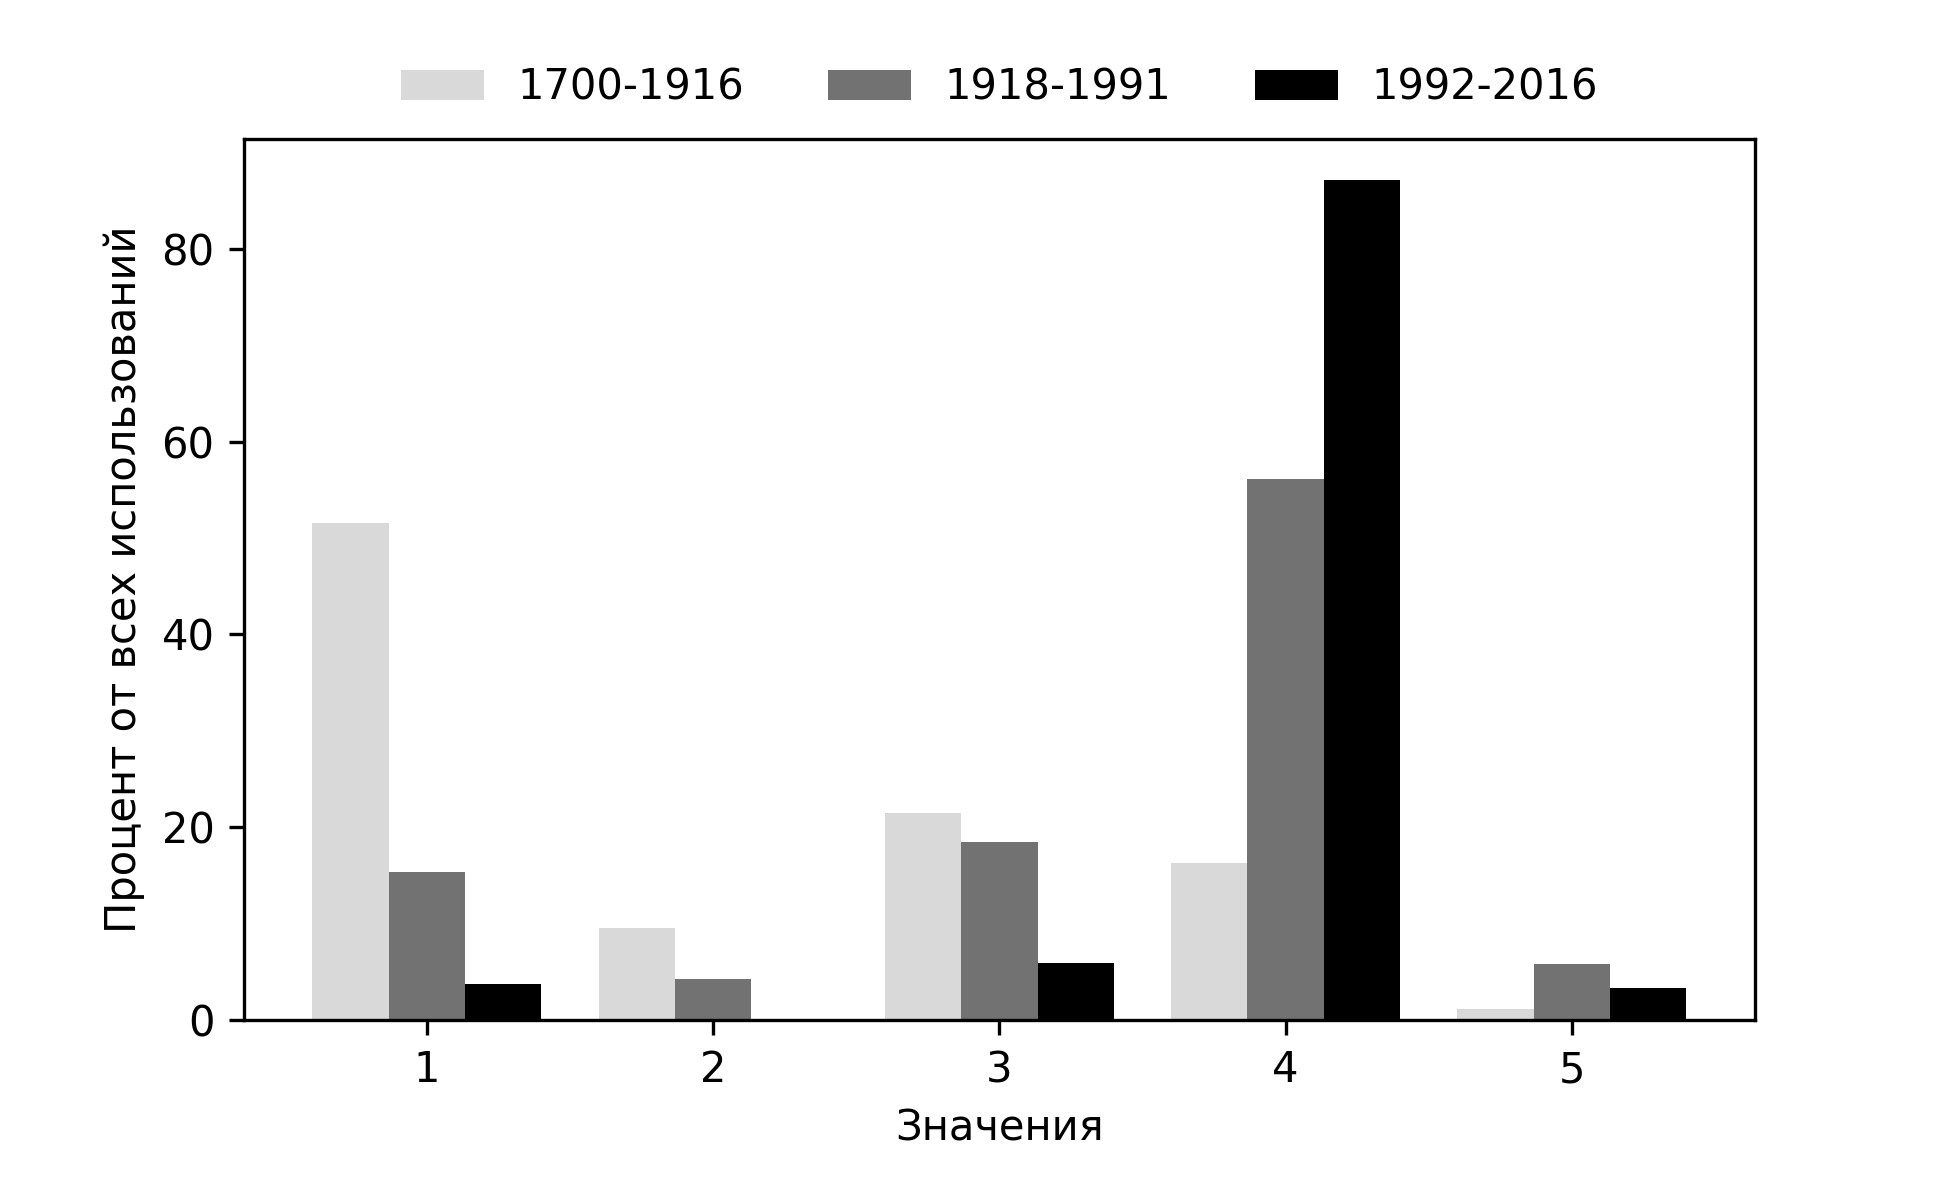
\includegraphics[width=0.8\textwidth]{img/visualizations/svalka_minimal}
	\caption{Изменение значений слова \textit{Свалка} (Параметры: eps=0.12, min\_samples=25)}
	\label{fig:Свалка}
\end{figure}

Значения для визуализации слова \textit{Свалка}:

\begin{enumerate}
    \item Столкновение, драка.
    \item Беспорядочное, беспорядочное движение, толкотня.
    \item Беспорядочная, беспорядочная схватка.
    \item Место, где свалены, свалены в кучу какие-либо отходы.
    \item То, что свалено, свалено в кучу.
\end{enumerate}

Перейдем к анализу определений.

Первое определение корректно сформулированы.
Остальные определения имеют разного рода ошибки.

\begin{itemize}
    \item ’Столкновение, драка.’ соответствует ’Всеобщая драка.’, так как
имеет общий смысловой элемент, а именно семы \textit{’столкновение’} и \textit{’драка’}.

    \item ’Место, где свалены, свалены в кучу какие-либо отходы.’ соответствует
’Место, куда свозят, выбрасывают мусор, нечистоты, негодные вещи.’,
так как включает те же семы \textit{’место’}, \textit{’свалены’}, \textit{’отходы’}.
Однако повторение слова \textit{свалены} является ошибкой в генерации.
\end{itemize}

\begin{itemize}
    \item ’Беспорядочное, беспорядочное движение, толкотня.’ частично соответствует
’Скопление людей, толпа.’, которое также указано в «Двух веках в двадцати словах» как ’Толпа, давка.’,
так как подразумевает собрание большого количества людей.
Однако повторение слова \textit{беспорядочное} является ошибкой в генерации,
что также относит определение к избыточным.

    \item ’Беспорядочная, беспорядочная схватка.’ соответствует
’Всеобщая драка.’, включает семы \textit{’потасовка’}, \textit{’с участием большого количества людей’}.
Повторение слова \textit{беспорядочная} является ошибкой в генерации,
соответственно данное определение будет определено как избыточное.

    \item ’То, что свалено, свалено в кучу.’ соответствует
‘Груда, куча, нагромождение чего-либо.’, так как оба определения акцентируют внимание
на неорганизованном скоплении чего-либо.
Повторение слова \textit{свалено} является ошибкой в генерации,
поэтому мы классифицируем это определение как имеющее избыточность.
\end{itemize}

Обобщённые значения, не найденные в визуализации:

\begin{itemize}
    \item ’Процесс сваливания’ также отсутствует в визуализации.
Это значение указывает на процесс, а не на результат, что могло быть причиной его отсутствия в предсказаниях модели.

    \item ’Вооруженное столкновение войск, битва’ отсутствует среди предложенных моделью значений.
Это значение является редким, что могло быть причиной его невключения в результат.
\end{itemize}

Определения, предложенные алгоритмом с повторением слов, далее будут написаны без повторения.

Таким образом, для лексемы \textit{свалка} представлено 1 корректное определение.
Среди ошибок присутствует:
\begin{itemize}
    \item Избыточность или чрезмерное использование общих фраз: 3
    \item Близкое значение, а также избыточность или чрезмерное использование общих фраз: 1
\end{itemize}

Перейдем к частотности значений.

В книге «Два века в двадцати значениях» как появившееся в 1900-ых годах указано
значение \textit{«Место для сбора мусора, помойка.»}, соответствующее четвёртому значению,
предложенному алгоритмом ’Место, где свалены, в кучу какие-либо отходы.’.
Как видно из графика результатов алгоритма, оно почти не используется в досоветский период,
но становится главным
с 60\% использования в советский период и доминирует в постсоветский с около 85\%.
Эти данные совпадают с тем, что говорится в книге, где утверждается 87\% использования
значения \textit{«Помойка.»} в 1998-1997 годы, 32\% для 1925-1949 годов.

Уменьшается же судя по графику преимущественно значение 1 (’Столкновение, драка.’),
которое падает с 50\% использований в досоветский период до 5\% в постсоветский.
В книге резульаты схожи.
Так, утверждается, что в 1875-1899 году слово имело значение ’Драка.’
в 71\% использований,
а к 1998-1997 значение упало до 12\%.

\noindent % Prevents indentation for this line to align the images at the left margin
\begin{figure}[H]
    \centering % Centers the images
    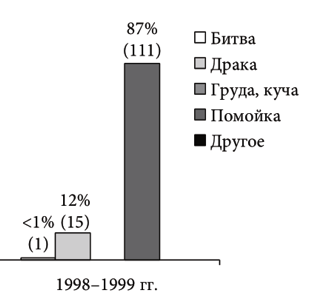
\includegraphics[width=0.32\textwidth]{img/book/Свалка 1998-1999}
    \hfill % Fills the space between the images
    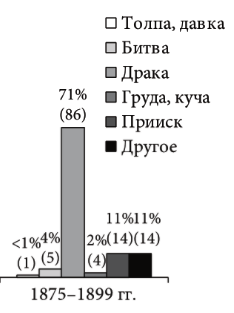
\includegraphics[width=0.32\textwidth]{img/book/Свалка 1875-1799}
    \hfill % Fills the space between the images
    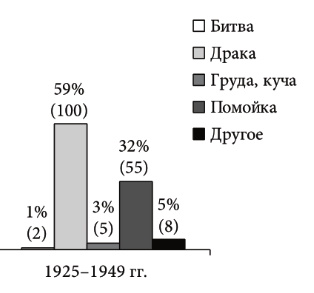
\includegraphics[width=0.32\textwidth]{img/book/Свалка 1925-1949}
    \caption{Визуализации для слова \textit{свалка} согласно~\cite{TwoCenturies}}
\end{figure}

Таким образом, модель довольно точно отражает реальное изменение значений слова \textit{свалка}
во времени, согласуясь с данными из толкового словаря и историческим исследованием.
Она адекватно выделяет как наиболее широко используемое сегодня значение,
связанное с местом сбора мусора,
так и менее очевидные значения, включая драку,
однако предложенные моделью определения имеют излишние повторения слов.

\section*{Сволочь}

В результате анализа семем лексемы \textit{сволочь} в толковых словарях были выделены шесть групп значений,
которые можно условно сформулировать следующим образом:

\begin{enumerate}
    \item Подлый, скверный человек; негодяй. \textit{Обманул-таки, сволочь.!}
(\textit{«Грубо. Скверный, подлый человек; негодяй.»} в БТС,
\textit{«Негодяй, мерзавец.»} в ТСО,
\textit{«Подлец»} в «Двух веках в двадцати словах»)

    \item Собирательное наименование для дрянных, подлых людей; сброд, подонки. \textit{Всякая сволочь.}
(\textit{«собир. Дрянные, подлые люди; сброд, подонки.»} в БТС,
\textit{«собир. Сброд, подлые люди.»} в ТСО,
\textit{«Сброд»} в «Двух веках в двадцати словах»)

    \item Военный сброд, разброд войска. \textit{Многочисленные колонны наши обратились в буйную сволочь, в которой солдаты разных полков были чужды один другому}
(\textit{«Вольница, военный сброд»} в «Двух веках в двадцати словах»)

    \item Малые люди, чернь, мелкая канцелярская чернь. \textit{...на другой день вся эта мелкая канцелярская сволочь явилась у меня в передней с поклонами, поздравлениями и доносами.}
(\textit{«Маленькие люди, чернь»} в «Двух веках в двадцати словах»)

    \item Сборище, компания. \textit{Вчера я обедал со всею сволочью здешних литераторов.}
(\textit{«Сборище»} в «Двух веках в двадцати словах»)

    \item Экспрессивное восклицание, выражающее негативные эмоции. \textit{Крепкое, сволочь! Аж в голову ступило...}
(\textit{«Экспрессивное восклицание»} в «Двух веках в двадцати словах»)
\end{enumerate}

\begin{figure}[H]
	\centering
	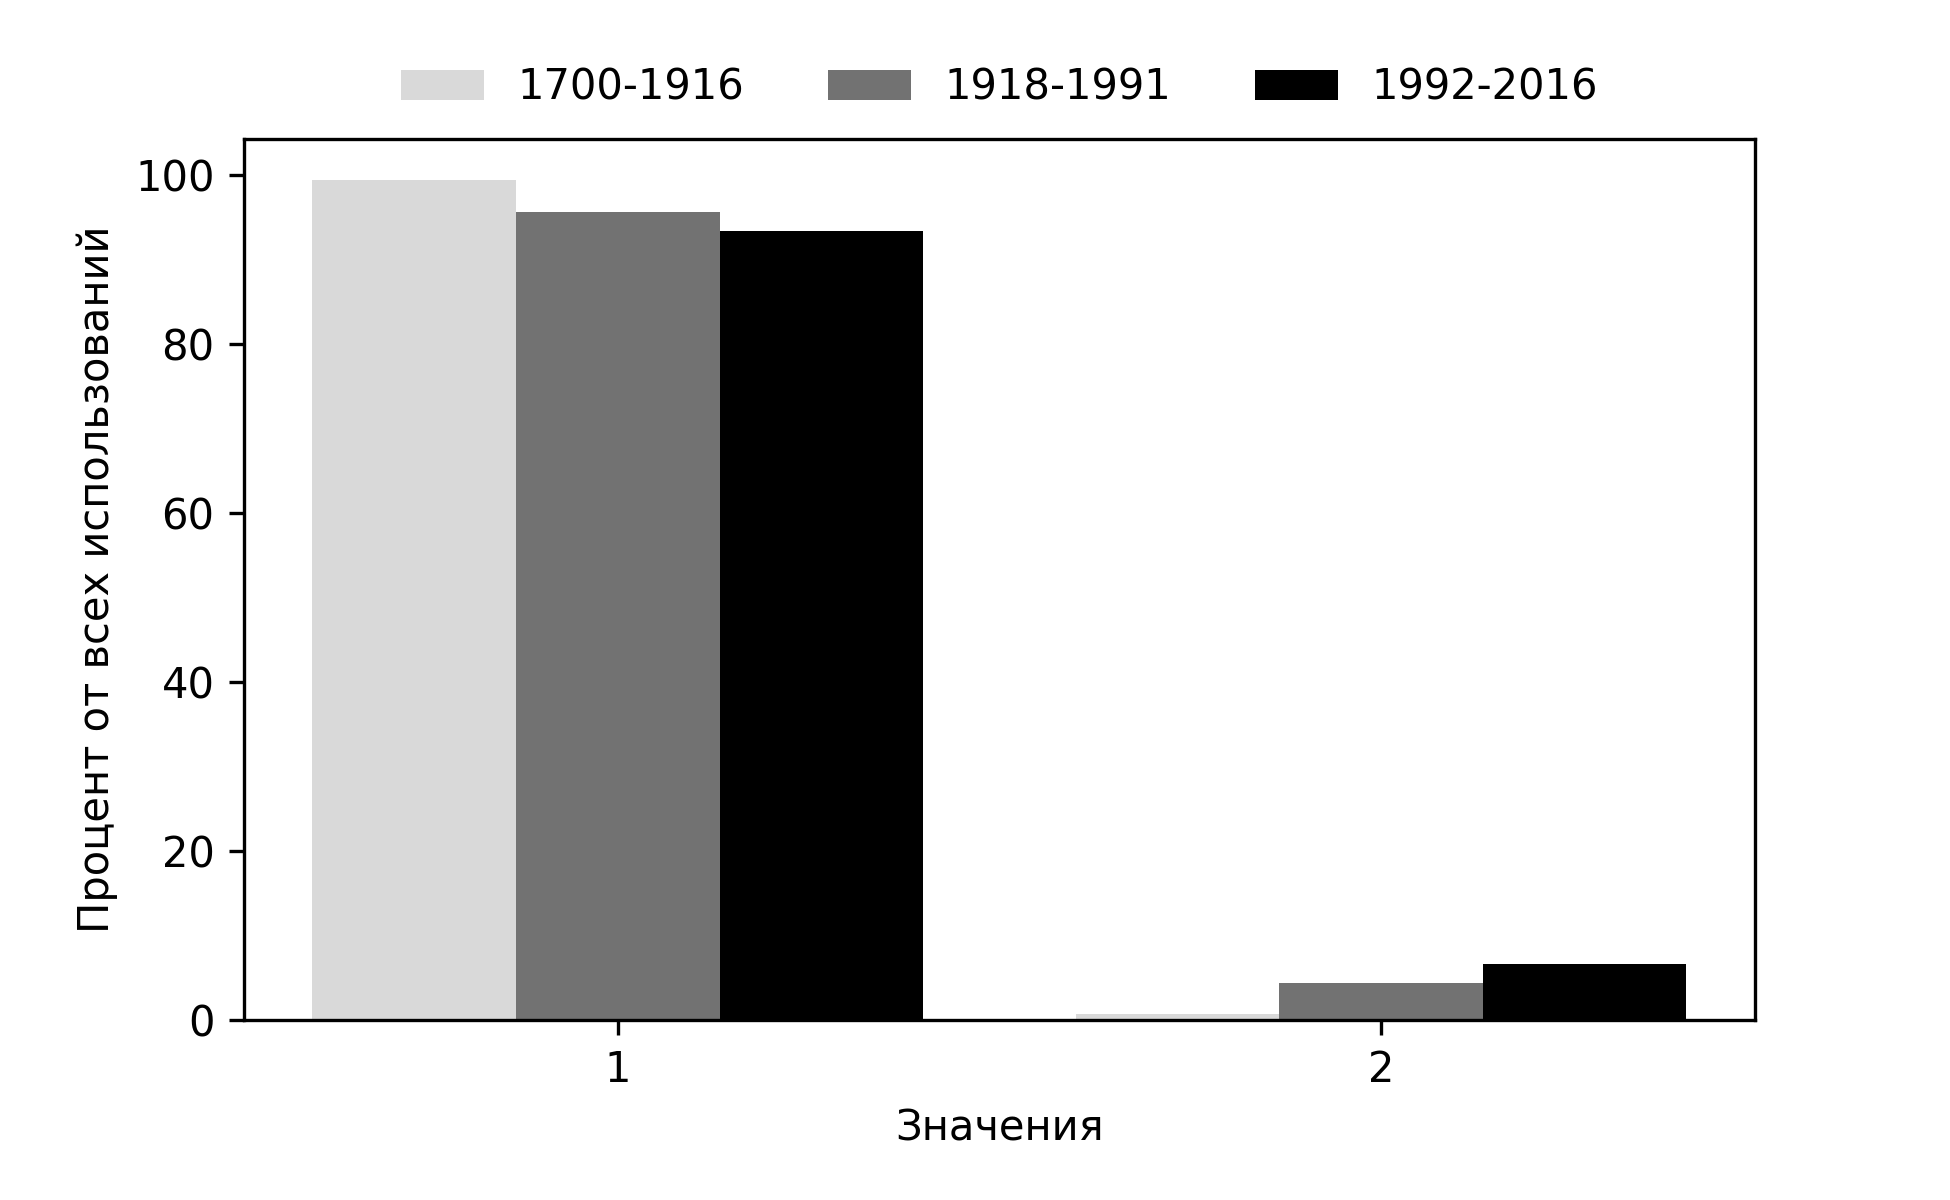
\includegraphics[width=0.8\textwidth]{img/visualizations/svoloch'_minimal}
	\caption{Изменение значений слова \textit{cволочь}}
	\label{fig:Сволочь}
\end{figure}

Значения для визуализации слова \textit{cволочь} (Параметры: eps=0.1, min\_samples=10).

\begin{enumerate}
    \item Употребляется как бранное слово.
%    \item Таща, доставить куда-либо.
    \item О подлом, гнусном человеке.
\end{enumerate}

\subsection*{Анализ значений слова \textit{сволочь}}

Первое и третье определения корректно сформулированы.
Второе определение не соответствует обобщенным значениям.

\begin{itemize}
    \item ’Употребляется как бранное слово.’ имеет общий смысловой элемент с
’Экспрессивное восклицание, выражающее негативные эмоции.’,
а именно семы \textit{’бранное слово’} и \textit{’экспрессивное восклицание’}.

    \item ’О подлом, гнусном человеке.’ полностью соответствует
    ’Подлый, скверный человек; негодяй.’, так как включает те же семы \textit{’подлый’}, \textit{’гнусный’}.
\end{itemize}

%\begin{itemize}
%    \item ’Таща, доставить куда-либо.’ является некорректным значением,
%    так как в обобщенных значениях нет упоминания о действии «тащить» или «доставлять».
%\end{itemize}

Обобщённые значения, не найденные в визуализации:
\begin{itemize}
    \item ’Собирательное наименование для дрянных, подлых людей; сброд, подонки’ отсутствует среди предложенных моделью значений.
Возможно, информации из контекста использований недостаточно для выявления этого значения.

    \item ’Военный сброд, разброд войска’ также отсутствует в визуализации.
Это может быть связано с редкостью использования данного значения в современных контекстах.

    \item ’Малые люди, чернь, мелкая канцелярская чернь’ также не представлено в визуализации,
что может указывать на недостаточное количество примеров с этим значением в датасете.

    \item ’Сборище, компания’ также не было явно выделено.
\end{itemize}

Таким образом, для лексемы \textit{сволочь} представлено 2 корректных определения.

Перейдем к частотности значений.

К сожалению, оба выделенных значения подпадают под значение ’Индивидуальное оскорбление.’
в книге «Два века в двадцати словах», поэтому анализ изменений значения
сделать не представляется возможным.

\section*{Стиль}

В результате анализа семем лексемы \textit{стиль} в толковых словарях были выделены следующие группы значений,
которые можно условно сформулировать следующим образом:

\begin{enumerate}
    \item Совокупность признаков, черт, приёмов, создающих целостный образ искусства определённого времени, направления, индивидуальной манеры художника.
(\textit{«Совокупность признаков, черт, создающих целостный образ искусства определённого времени, направления, индивидуальной манеры художника в отношении идейного содержания и художественной формы.»} в БТС,
\textit{«Совокупность черт, близость выразительных художественных приёмов и средств, обусловливающие собой единство какого-н. направления в творчестве.»} в ТСО,
\textit{«Стилем называют жанровую и тематическую направленность художественного произведения.»} и \textit{«Стилем называют совокупность литературных приёмов, характерных для какого-либо направления, жанра, произведения.»} в ТСД,
\textit{«Особенности направления архитектуры»} в «Двух веках в двадцати словах»)

    \item Способ летоисчисления. \textit{Новый стиль.}
(\textit{«Способ летосчисления.»} в БТС, ТСО и ТСД,
\textit{«Способ летоисчисления»} в «Двух веках в двадцати словах»)

    \item Способ, метод, совокупность приёмов осуществления какой-либо деятельности, работы. \textit{Стиль руководства.}
(\textit{«Способ осуществления чего-л., характер деятельности, работы в их отличительных признаках.»} в БТС,
\textit{«Метод, совокупность приёмов какой-н. работы, деятельности, поведения.»} в ТСО,
\textit{«Стилем называется способ осуществления чего-либо.»} в ТСД)

    \item Совокупность приёмов использования языковых средств. \textit{Романтический стиль.}
(\textit{«Совокупность приёмов использования средств языка, характерная для какого-л. писателя или литературного произведения, направления, жанра.»} в БТС,
\textit{«Совокупность приёмов использования языковых средств для выражения тех или иных идей, мыслей в различных условиях речевой практики, слог.»} и \textit{«Совокупность приёмов использования языковых средств, а также вообще средства художественной выразительности, определяющие своеобразие творчества писателя, отдельного произведения.»} в ТСО,
\textit{«Характеристика языковых средств»} в «Двух веках в двадцати словах»)

    \item Индивидуальная манера художника, писателя. \textit{Свой стиль Щедрин называет эзоповским.}
(\textit{«Стилем называют индивидуальную авторскую манеру, которая ощущается читателем, зрителем в нескольких произведениях одного автора.»} в ТСД,
\textit{«Черты, свойственные конкретному человеку (например, деятелю искусства)»} в «Двух веках в двадцати словах»)

    \item Совокупность наиболее характерных черт в искусстве какого-либо народа, страны, региона. \textit{Русский стиль.}
(\textit{«совокупность наиболее общих черт в искусстве какого-л. народа, страны, региона, отличающихся от искусства соседних народов и т.п..»} в БТС,
\textit{«Стилем называют совокупность наиболее характерных черт в искусстве какого-либо народа, страны и т. п.»} в ТСД)

    \item Манера словесного изложения. \textit{Лаконичный стиль.}
(\textit{«Построение речи в соответствии с нормами литературного языка, манера словесного изложения.»} в БТС,
\textit{«Стилем называют чью-либо манеру словесного изложения какой-либо информации.»} в ТСД)

    \item Функциональная разновидность литературного языка. \textit{Официально-деловой стиль.}
(\textit{«Функциональная разновидность литературного языка.»} в БТС,
\textit{«Стилем называют функциональную разновидность литературного языка.»} в ТСД)

    \item Характерная манера совершения движения, в т.ч. в спорте. \textit{Стили гребли.}
(\textit{«Совокупность признаков, черт, приёмов, выделяющих какую-л. вещь, предмет на фоне аналогичных и образующих их суть (в спорте).»} в БТС,
\textit{«Стилем называют характерную манеру совершения движения.»} в ТСД)

    \item Модное веяние в одежде, совокупность признаков, черт вещей, одежды. \textit{Джинсовый стиль.}
(\textit{«Совокупность признаков, черт, отличающих направление, вещь от других (в моде, в одежде).»} в БТС,
\textit{«Стилем называют модное веяние, которое воспринято многими.»} в ТСД)

    \item Изменяющаяся социальная форма жизни, деятельности. \textit{Московский стиль жизни.}
(\textit{«Совокупность признаков общественной жизни, активности в тот или иной период.»} в БТС,
\textit{«Стилем называют изменяющуюся социальную форму жизни, деятельности.»} в ТСД)

    \item Индивидуальная манера поведения, общения, одежды и т.п. \textit{Стиль поведения, общения.}
(\textit{«Индивидуальная манера осуществления какой-л. деятельности, работы, проявления личных качеств в разговоре, поведении, одежде и т.п.»} в БТС,
\textit{«Стилем называют изменяющуюся индивидуальную форму жизни, деятельности.»} и \textit{«Манера, совокупность особенностей по отношению к широкому кругу явлений (поведение, одежда, взгляды, внешность, интерьер)»} в «Двух веках в двадцати словах»)

%    \item В стиле кого-либо, чего-либо (следование примеру, подражание кому-либо, чему-либо).
%(\textit{«Если кто-либо делает что-либо в стиле кого-либо, чего-либо, то это означает, что этот человек следует примеру кого-либо, подражает чему-либо и т. п.»} в ТСД)

\end{enumerate}

\begin{figure}[H]
	\centering
	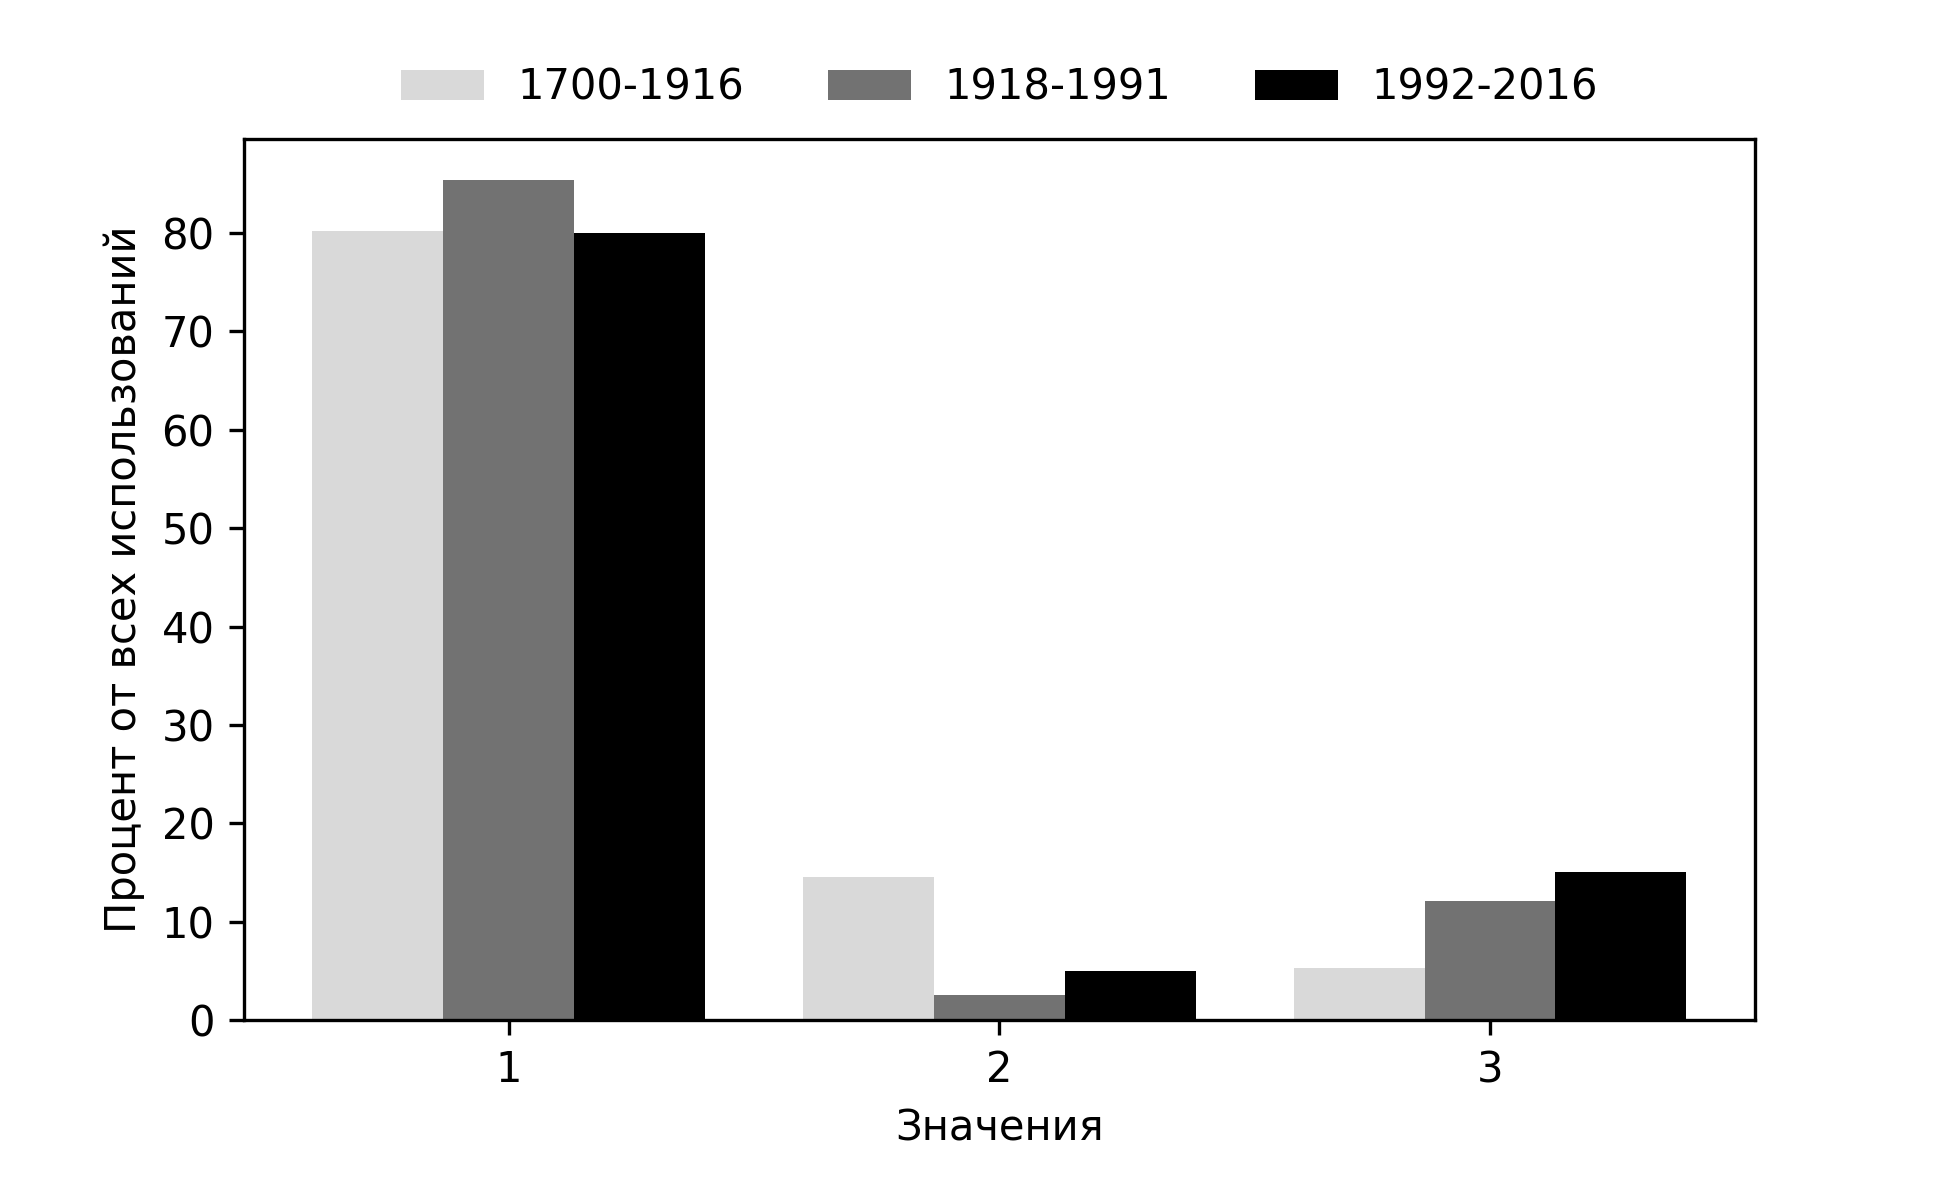
\includegraphics[width=0.8\textwidth]{img/visualizations/stil'_minimal}
	\caption{Изменение значений слова \textit{стиль}}
	\label{fig:Стиль_книга}
\end{figure}

Значения для визуализации слова «Стиль» (Параметры: eps=0.15, min\_samples=25).

\begin{enumerate}
    \item Совокупность художественных приемов, характерных для какого-либо искусства, литературы и т. п.
    \item Система летосчисления, принятая в какой-л. стране, а также время по этой системе.
    \item Характер, манера, образ действий, поведения кого-либо.
\end{enumerate}

Перейдем к анализу определений.

Определения корректно сформулированы.

\begin{itemize}
    \item ’Совокупность художественных приемов, характерных для какого-либо искусства, литературы и т. п.’ имеет общий смысловой элемент с
’Совокупность признаков, черт, приёмов, создающих целостный образ искусства определённого времени, направления, индивидуальной манеры художника.’
’Индивидуальная манера художника, писателя.’
’Совокупность наиболее характерных черт в искусстве какого-либо народа, страны, региона.’
’Совокупность приёмов использования языковых средств.’
а именно семы \textit{’совокупность’}, \textit{’приемы’}, \textit{’искусство’}, \textit{’литература’}.

    \item ’Система летосчисления, принятая в какой-л. стране, а также время по этой системе’ полностью соответствует
’Способ летоисчисления.’, так как включает те же семы \textit{’система’}, \textit{’летосчисление’}, \textit{’страна’}.
\end{itemize}

\begin{itemize}
    \item ’Характер, манера поведения кого-либо.’ наиболее близко к
’Индивидуальная манера поведения, общения, одежды и т.п.’
\end{itemize}

Обобщённые значения, не найденные в визуализации:
\begin{itemize}
    \item ’Функциональная разновидность литературного языка.’ отсутствует среди предложенных моделью значений.
Можно предположить, что информации из контекста использований недостаточно для отделения этого значения от ’Совокупность художественных приемов, характерных для какого-либо искусства, литературы и т. п.’.

    \item ’Модное веяние в одежде, совокупность признаков, черт вещей, одежды.’ также отсутствует в визуализации.
Однако, модель способна на выделение данного значения.

    \item ’Изменяющаяся социальная форма жизни, деятельности.’ и ’Характерная манера совершения движения, в т.ч. в спорте.’ также отсутствуют.
Возможно, эти значения не были включены из-за их меньшей частоты в исследуемом материале.
\end{itemize}

Таким образом, для лексемы \textit{стиль} представлены 3 корректные определения.

Перейдем к частотности значений.

К сожалению, в книге «Два века в двадцати словах» указано,
что все значения слова «стиль» появились в досоветский период,
а также все графики даны только для этого периода.
Однако в книге говорится, что частота употребления значения ’Способ летоисчисления.’
снижается значительно с досоветского периода, что согласуется с данными нашего исследования.
В остальном, представляется затруднительным сравнение результатов модели с данными из книги.

\begin{figure}[H]
    \centering % Centers the images
    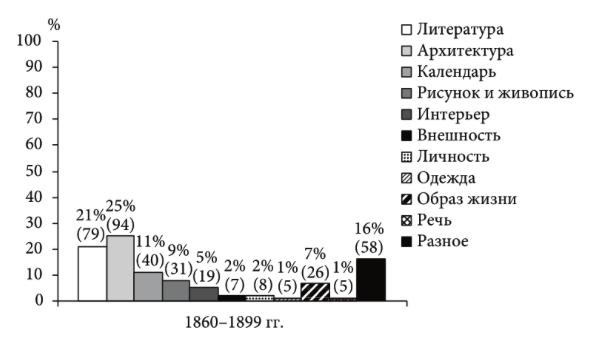
\includegraphics[width=0.32\textwidth]{img/book/stil'/1860-1899}
    \caption{Визуализации для слова \textit{стиль} для 1860-1899 согласно~\cite{TwoCenturies}}
    \label{fig:Стиль}
\end{figure}

\section*{Тётка}

В результате анализа семем лексемы \textit{тётка} в толковых словарях были выделены следующие группы значений:

\begin{enumerate}
    \item Вообще женщина. \textit{Уселись тётки на лавочке.}
(\textit{«Обо всякой взрослой женщине.»} в БТС,
\textit{«Тёткой грубо называют женщину или девушку.»} в ТСД,
\textit{«Вообще женщина (чаще пожилая).»} в ТСО,
\textit{«Женщина (вне контекста обращения)»} в «Двух веках в двадцати словах»)

    \item Сестра отца или матери, а также жена дяди.  \textit{Родная, двоюродная тётка.}
(\textit{«Сестра отца или матери, а также жена дяди.»} в ТСО,
\textit{«Тёткой называют сестру матери или отца.»} в ТСД,
\textit{«=Тётя (1 зн.).»} в БТС,
\textit{«Сестра матери.»} в «Двух веках в двадцати словах»)

    \item Обращение к незнакомой женщине. \textit{— Не хлопочи, тётка, — сказал Алексей, войдя в избу.}
(\textit{«Обращение к незнакомой женщине (ед. или мн. ч.)»} в «Двух веках в двадцати словах»)

    \item Незнатная женщина, употребляется вместе с именем.
(\textit{«Называние незнатной женщины в форме «тётка + имя»»} в «Двух веках в двадцати словах»)
%    \item Фразеологизм «Голод не тётка».
%    (\textit{«Голод не тётка (Погов.)»} в БТС,
%    \textit{«Голод не т. (посл. о проголодавшемся; шутл.)»} в ТСО,
%    \textit{«Фраза Голод не тётка употребляется в том случае, если речь идёт о чьём-либо нестерпимом желании поесть, утолить голод.»} в ТСД)
%
    \item Карточная игра. \textit{Играют в «тётку».}
(\textit{«Карточная игра»} в «Двух веках в двадцати словах»)
\end{enumerate}

\begin{figure}[H]
	\centering
	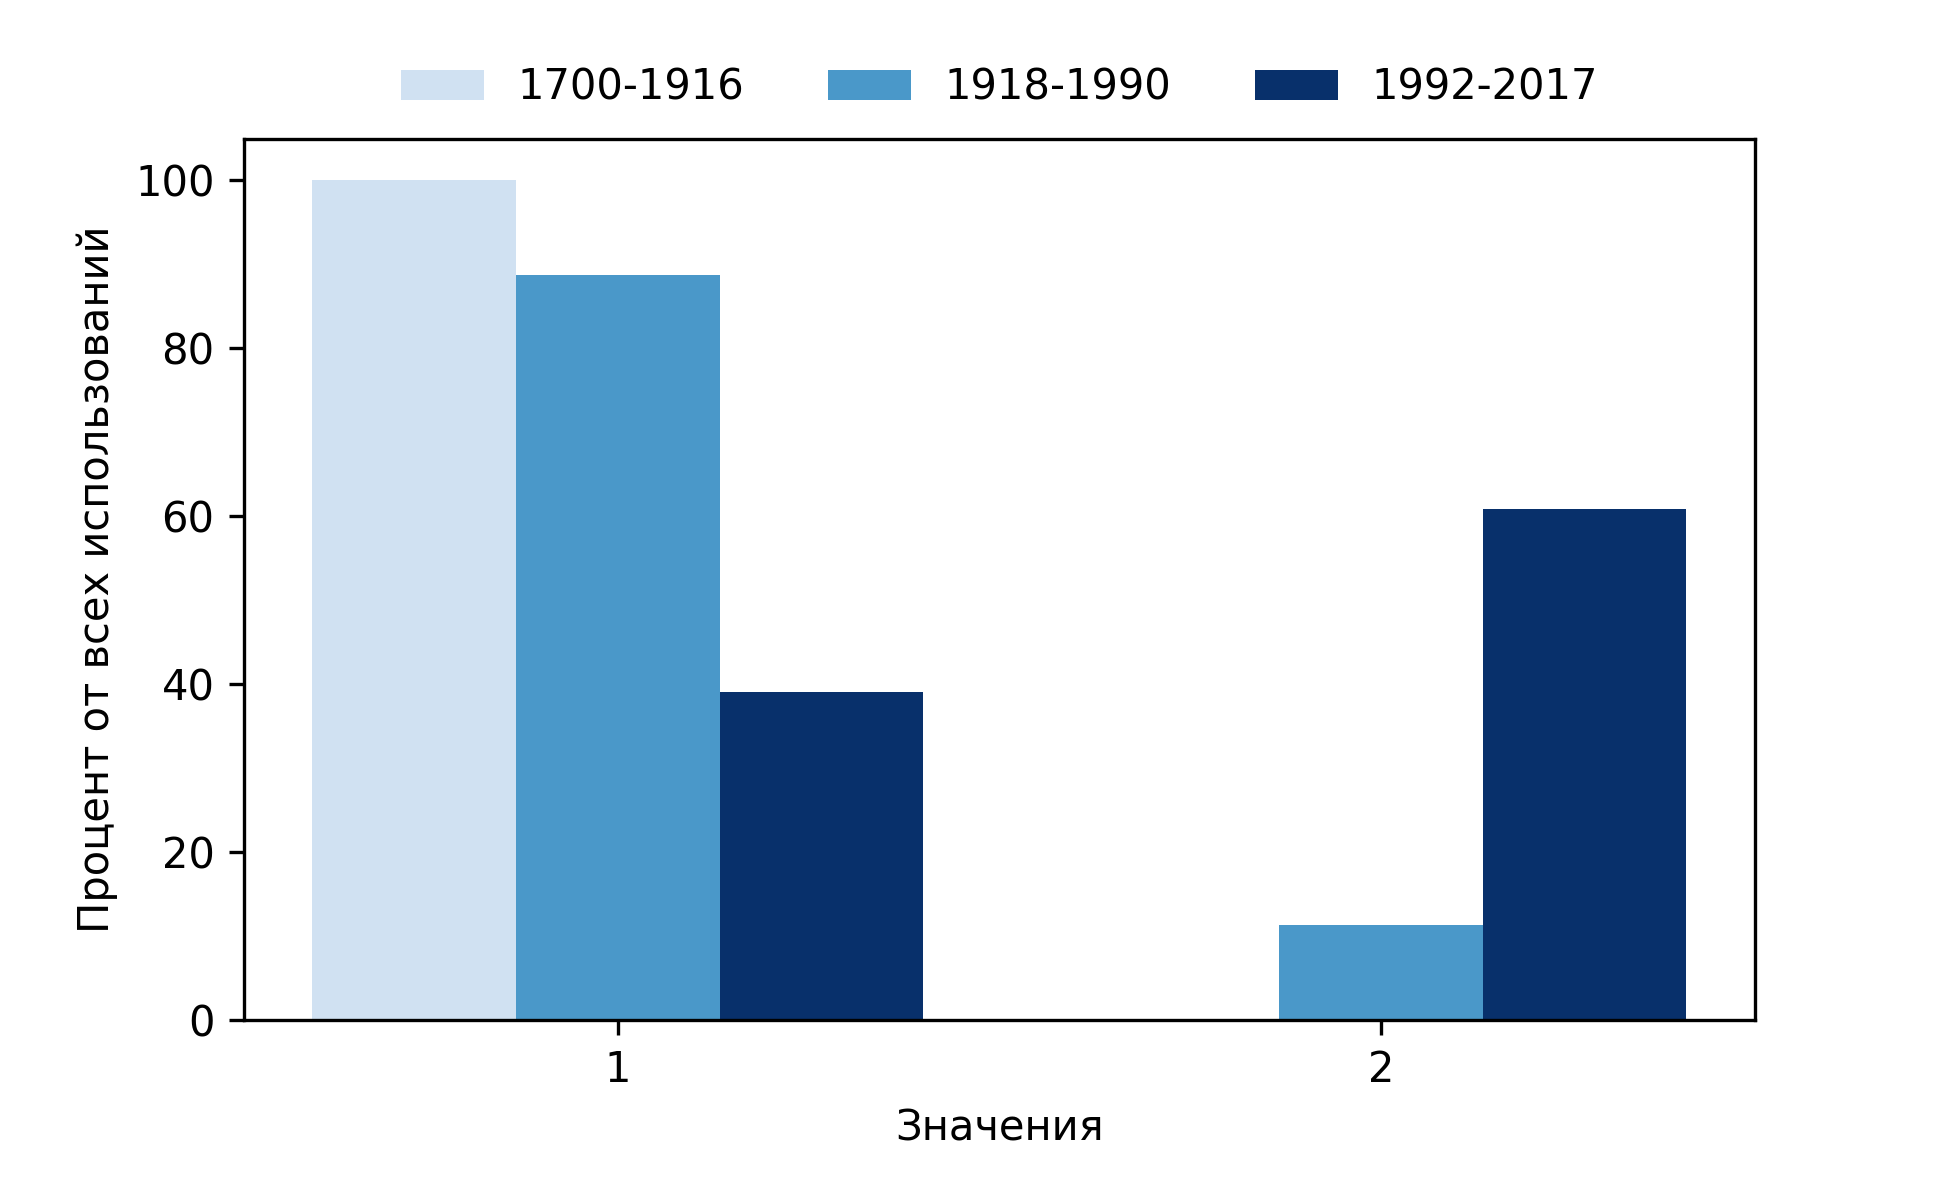
\includegraphics[width=0.8\textwidth]{img/visualizations/tetka_minimal}
	\caption{Изменение значений слова \textit{тётка}}
	\label{fig:Тётка}
\end{figure}

Значения для визуализации слова «Тётка» (Параметры: eps=0.1, min\_samples=15).

\begin{enumerate}
    \item Родная сестра отца или матери.
    \item Женщина средних лет.
\end{enumerate}

\subsection*{Анализ значений слова \textit{тётка}}

Первое определение корректно сформулировано.
Второе определение имеет слишком узкое значение, так как в словарях значение охватывает всех взрослых женщин,
а не только женщин средних лет.

\begin{itemize}
    \item ’Родная сестра отца или матери.’ имеет общий смысловой элемент с
’Сестра отца или матери, а также жена дяди.’, а именно семы «сестра» и «отец или мать».

    \item ’Женщина средних лет.’ соответствует ’Вообще женщина.’, хоть и более узкое,
так как обобщенное определения включает всех женщин, а не только женщин средних лет.
Сема «средних лет» делает его слишком узким.
\end{itemize}

Обобщённые значения, не найденные в визуализации:
\begin{itemize}
    \item ’Обращение к незнакомой женщине.’, как и ’Незнатная женщина.’ моделью отдельно от
’Женщина средних лет.’ не выделяется.

    \item ’Карточная игра’ также отсутствует в визуализации.
Его отсутствие обусловлено тем, что это значение не так часто встречается в исследуемом корпусе.
Данное определение указано только в «Двух веках в двадцати словах», где приводятся только
единичные использования слова в этом значении, не влияющие в целом на статистику значений.
\end{itemize}

Таким образом, для лексемы \textit{тётка} представлено 1 корректное определение.
Среди ошибок присутствует:
\begin{itemize}
    \item Избыточно конкретизированные: 1
\end{itemize}

Перейдем к частотности значений.

Главным изменением для слова \textit{тётка} является появление в конце советского периода
его использования по отношению ко всем женщинам, а не только родственницам (30\% для 1980-1985 гг.
и около 5\% для 1910-1920 и 1940-1954 гг.), что приводится в графиках снизу.
К сожалению, в книге не приводится информация об использовании слова в постсоветский период.
Данные из нашей визуализации согласуются с вышеописанными изменениями.
Так, значение ’Женщина средних лет.’ появляется в советский период с около 10\%
использований и выходит на лидирующие позиции в постсоветский период с больше 60\%.

\noindent % Prevents indentation for this line to align the images at the left margin
\begin{figure}[H]
    \centering % Centers the images
    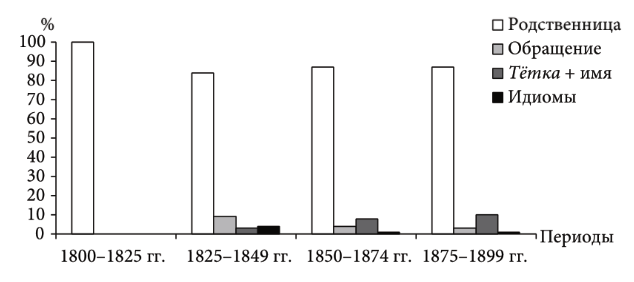
\includegraphics[width=0.8\textwidth]{img/book/tetka/1800-1899}
    \caption{График для слова \textit{тётка} для 1800-1899 согласно~\cite{TwoCenturies}}
\end{figure}

\begin{figure}[H]
    \centering % Centers the images
    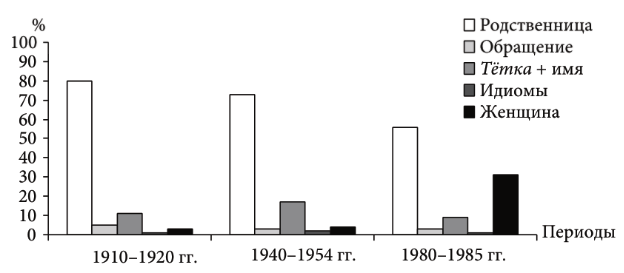
\includegraphics[width=0.8\textwidth]{img/book/tetka/1910-1985}
    \caption{График для слова \textit{тётка} для 1910-1985 согласно~\cite{TwoCenturies}}
\end{figure}

Таким образом, алгоритм полностью отражает значения, в которых использовалось
слово \textit{тётка}, согласуясь с данными из толкового словаря и историческим исследованием.

\section*{Червяк}

В результате анализа семем лексемы \textit{червяк} в толковых словарях были выделены четыре группы значений,
которые можно условно сформулировать следующим образом:

\begin{enumerate}
    \item Маленькое беспозвоночное животное.
    (\textit{«=Червь (1.Ч.; 1-2 зн.).»} в БТС,
    \textit{«То же, что червь.»} в ТСО,
    \textit{«Маленькое беспозвоночное животное»} в «Двух веках в двадцати словах»)

    \item Ничтожное, жалкое создание.
    (\textit{«О жалком, ничтожном человеке (презр)»} в ТСО,
    \textit{«Ничтожное создание»} в «Двух веках в двадцати словах»)

    \item Тревожное, мучительное чувство.
    (\textit{«О постоянном наличии какого-л. чувства, состояния, плохо воздействующего на кого-л.»} в БТС,
\textit{«Внутренний паразит»} в «Двух веках в двадцати словах»)

    \item Техническое приспособление в виде винта для передачи движения.
    (\textit{«Проф. Червячная передача; деталь механизма для такой передачи.»} в БТС,
    \textit{«Зубчатое колесо в форме винта для передачи движения в нек-рых механизмах (спец.)»} в ТСО,
    \textit{«Техническое приспособление»} в «Двух веках в двадцати словах»)
\end{enumerate}

\begin{figure}[H]
	\centering
	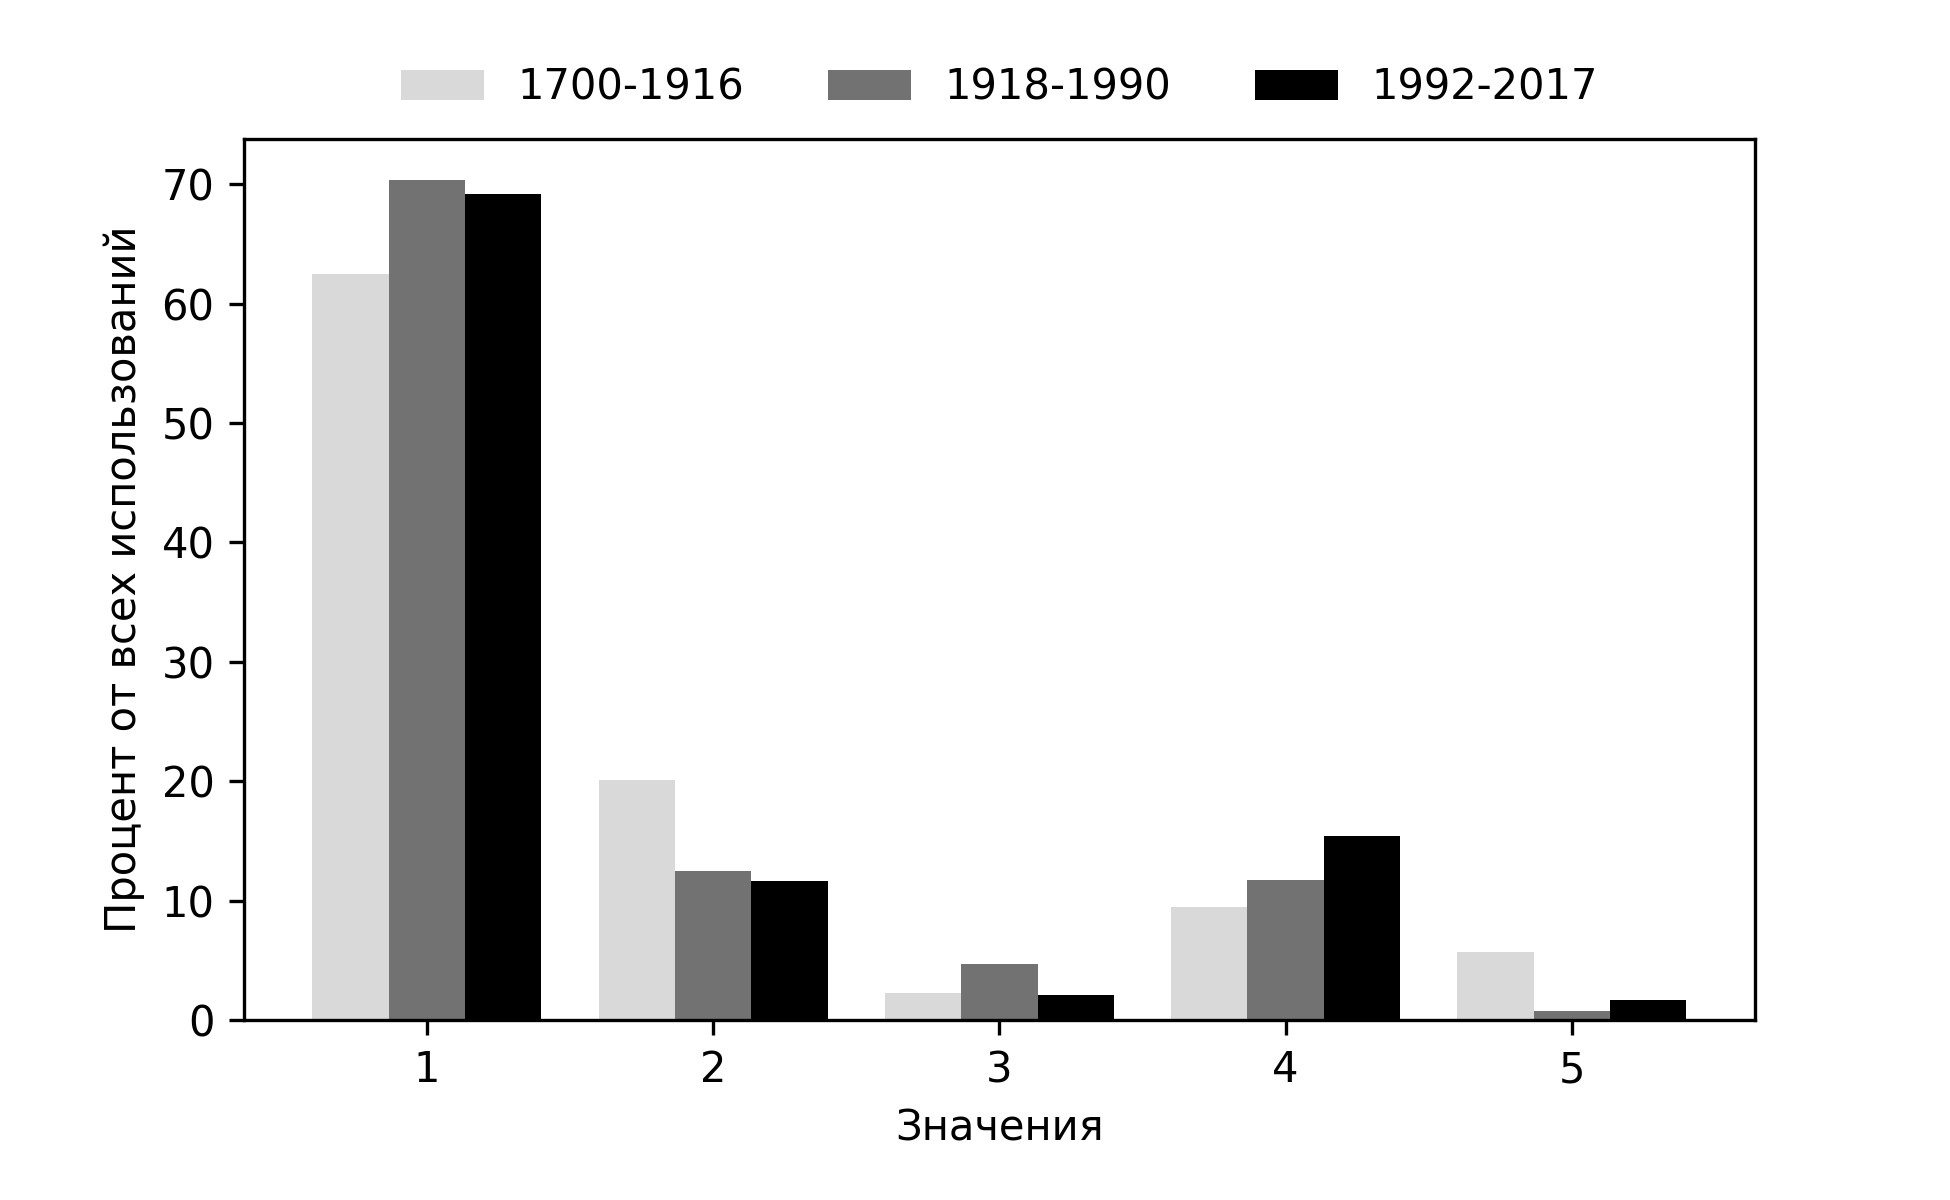
\includegraphics[width=0.8\textwidth]{img/visualizations/chervjak_minimal}
	\caption{Изменение значений слова \textit{червяк}}
	\label{fig:Червяк}
\end{figure}

Значения для визуализации слова «Червяк» (Параметры: eps=0.16, min\_samples=10).

\begin{enumerate}
    \item Насекомое, похожее на червя, а также его личинка.
    \item О мелком, ничтожном человеке.
    \item Употребляется как бранное слово.
    \item О ком-, чем-либо маленьком, тонком, извивающемся.
    \item О каком-л. неприятном, мучительном чувстве, испытываемом кем-л.
\end{enumerate}

\subsection*{Анализ значений слова \textit{червяк}}

Первое, второе и пятое определения корректно сформулированы.
Третье и четвертое определения не соответствуют обобщенным значениям.

\begin{itemize}
    \item ’Насекомое, похожее на червя, а также его личинка.’ имеет общий смысловой элемент с
’Маленькое беспозвоночное животное.’, а именно семы «маленькое», «животное».
Тем не менее, оно содержит значительные ошибки, червяк не является насекомым, а также содержит
ссылку на самого себя (червя).

    \item ’О мелком, ничтожном человеке.’ соответствует
’Ничтожное, жалкое создание.’, так как включает те же семы «ничтожность», «жалкость».

    \item ’О каком-л. неприятном, мучительном чувстве, испытываемом кем-л.’ соответствует
’Тревожное, мучительное чувство.’, так как включает семы «неприятное», «мучительное» и
«чувство».
\end{itemize}

\begin{itemize}
    \item ’Употребляется как бранное слово.’ является близким значением к
’Ничтожное, жалкое создание.’, так как бранное слово может указывать на презрение,
но не полностью соответствует исходному значению.

    \item ’О ком-, чем-либо маленьком, тонком, извивающемся.’ является близким значением к
’Маленькое беспозвоночное животное.’, которое не раскрывает отличительные стороны денотата.
\end{itemize}

Обобщённые значения, не найденные в визуализации:
\begin{itemize}
    \item ’Техническое приспособление в виде винта для передачи движения.’ отсутствует среди
предложенных моделью значений.
Модель способна на выделение этого значения, сгенерировав
’металлический стержень, служащий для передачи вращательного движения’ для вхождения
\textit{При установке киноаппарата в боксе надо следить за тем, чтобы червячное колесо и
червяк вошли в зацепление.}
Вероятно, модель не распознала это значение из-за его редкости в общем корпусе текстов.
\end{itemize}

Таким образом, для лексемы \textit{червяк} представлены 2 корректных определения.
Среди ошибок присутствуют:
\begin{itemize}
    \item Близкие значения: 3
\end{itemize}

Перейдем к частотности значений.

В книге «Два века в двадцати словах» не даётся графиков изменения частоты использования значений
для слова \textit{червяк}, однако упоминается о том, что значения
’Ничтожное, жалкое создание.’ и ’Тревожное, мучительное чувство.’
реже используются со временем, особенно во второй половине XX века.
Эти данные подтверждаются в нашей визуализации, где использование
’О мелком, ничтожном человеке.’ падает с 20\% в досоветский период до 10\% в советский и постсоветский,
а также использование ’О каком-л. неприятном, мучительном чувстве, испытываемом кем-л.’
уменьшается с около 8\% в досоветский период до 1-2\% в советский и 3\% в постсоветский.

Таким образом, алгоритм в целом отражает значения, в которых использовалось
слово \textit{червяк}, согласуясь историческим исследованием, но допуская различного рода ошибки
в 3 из 5 сгенерированных определениях.

\chapter{Обучение модели}

\begin{longtable}{ll}
\caption{LoRa параметры} \\
\hline
\textbf{Параметр} & \textbf{Значение} \\
\hline
r & 32 \\
lora\_alpha & 64 \\
lora\_dropout & 0.1 \\
\hline
\end{longtable}

\begin{longtable}{ll}
\caption{Trainer параметры} \\
\hline
\textbf{Параметр} & \textbf{Значение} \\
\hline
learning\_rate & 1e-3 \\
lr\_scheduler\_type & linear \\
batch\_size & 16 \\
gradient\_checkpointing & true \\
gradient\_accumulation\_steps & 1 \\
weight\_decay & 0.1 \\
optimizer & adafactor \\
num\_train\_epochs & 6 \\
\hline
\end{longtable}

\chapter{Дообучение векторизатора}

\begin{table}[H]
\centering
\begin{tabular}{|l|l|}
\hline
\textbf{Hyperparameter}    & \textbf{Value} \\ \hline
Batch size                 & 32    \\ \hline
Loss function              & CosineSimilarityLoss \\ \hline
Epochs                     & 2     \\ \hline
Warmup steps               & 100   \\ \hline
Evaluation steps           & 50    \\ \hline
Training data split ratio  & 80/20 \\ \hline
Random seed                & 42    \\ \hline
\end{tabular}
\caption{Hyperparameters for model training}
\label{tab:hyperparameters}
\end{table}
